% Options for packages loaded elsewhere
% Options for packages loaded elsewhere
\PassOptionsToPackage{unicode}{hyperref}
\PassOptionsToPackage{hyphens}{url}
%
\documentclass[
  10pt,
  ignorenonframetext,
  aspectratio=169,
  spanish,
]{beamer}
\newif\ifbibliography
\usepackage{pgfpages}
\setbeamertemplate{caption}[numbered]
\setbeamertemplate{caption label separator}{: }
\setbeamercolor{caption name}{fg=normal text.fg}
\beamertemplatenavigationsymbolsempty
% remove section numbering
\setbeamertemplate{part page}{
  \centering
  \begin{beamercolorbox}[sep=16pt,center]{part title}
    \usebeamerfont{part title}\insertpart\par
  \end{beamercolorbox}
}
\setbeamertemplate{section page}{
  \centering
  \begin{beamercolorbox}[sep=12pt,center]{section title}
    \usebeamerfont{section title}\insertsection\par
  \end{beamercolorbox}
}
\setbeamertemplate{subsection page}{
  \centering
  \begin{beamercolorbox}[sep=8pt,center]{subsection title}
    \usebeamerfont{subsection title}\insertsubsection\par
  \end{beamercolorbox}
}
% Prevent slide breaks in the middle of a paragraph
\widowpenalties 1 10000
\raggedbottom
\AtBeginPart{
  \frame{\partpage}
}
\AtBeginSection{
  \ifbibliography
  \else
    \frame{\sectionpage}
  \fi
}
\AtBeginSubsection{
  \frame{\subsectionpage}
}
\usepackage{iftex}
\ifPDFTeX
  \usepackage[T1]{fontenc}
  \usepackage[utf8]{inputenc}
  \usepackage{textcomp} % provide euro and other symbols
\else % if luatex or xetex
  \usepackage{unicode-math} % this also loads fontspec
  \defaultfontfeatures{Scale=MatchLowercase}
  \defaultfontfeatures[\rmfamily]{Ligatures=TeX,Scale=1}
\fi
\usepackage{lmodern}

\usetheme[]{Madrid}
\usecolortheme[]{dolphin}
\usefonttheme[]{professionalfonts}
\usefonttheme{serif} % use mainfont rather than sansfont for slide text
\ifPDFTeX\else
  % xetex/luatex font selection
  \setmainfont[]{DejaVu Sans}
  \setsansfont[]{DejaVu Sans}
  \setmonofont[]{DejaVu Sans Mono}
\fi
% Use upquote if available, for straight quotes in verbatim environments
\IfFileExists{upquote.sty}{\usepackage{upquote}}{}
\IfFileExists{microtype.sty}{% use microtype if available
  \usepackage[]{microtype}
  \UseMicrotypeSet[protrusion]{basicmath} % disable protrusion for tt fonts
}{}
\makeatletter
\@ifundefined{KOMAClassName}{% if non-KOMA class
  \IfFileExists{parskip.sty}{%
    \usepackage{parskip}
  }{% else
    \setlength{\parindent}{0pt}
    \setlength{\parskip}{6pt plus 2pt minus 1pt}}
}{% if KOMA class
  \KOMAoptions{parskip=half}}
\makeatother

\usepackage{color}
\usepackage{fancyvrb}
\newcommand{\VerbBar}{|}
\newcommand{\VERB}{\Verb[commandchars=\\\{\}]}
\DefineVerbatimEnvironment{Highlighting}{Verbatim}{commandchars=\\\{\}}
% Add ',fontsize=\small' for more characters per line
\usepackage{framed}
\definecolor{shadecolor}{RGB}{241,243,245}
\newenvironment{Shaded}{\begin{snugshade}}{\end{snugshade}}
\newcommand{\AlertTok}[1]{\textcolor[rgb]{0.68,0.00,0.00}{#1}}
\newcommand{\AnnotationTok}[1]{\textcolor[rgb]{0.37,0.37,0.37}{#1}}
\newcommand{\AttributeTok}[1]{\textcolor[rgb]{0.40,0.45,0.13}{#1}}
\newcommand{\BaseNTok}[1]{\textcolor[rgb]{0.68,0.00,0.00}{#1}}
\newcommand{\BuiltInTok}[1]{\textcolor[rgb]{0.00,0.23,0.31}{#1}}
\newcommand{\CharTok}[1]{\textcolor[rgb]{0.13,0.47,0.30}{#1}}
\newcommand{\CommentTok}[1]{\textcolor[rgb]{0.37,0.37,0.37}{#1}}
\newcommand{\CommentVarTok}[1]{\textcolor[rgb]{0.37,0.37,0.37}{\textit{#1}}}
\newcommand{\ConstantTok}[1]{\textcolor[rgb]{0.56,0.35,0.01}{#1}}
\newcommand{\ControlFlowTok}[1]{\textcolor[rgb]{0.00,0.23,0.31}{\textbf{#1}}}
\newcommand{\DataTypeTok}[1]{\textcolor[rgb]{0.68,0.00,0.00}{#1}}
\newcommand{\DecValTok}[1]{\textcolor[rgb]{0.68,0.00,0.00}{#1}}
\newcommand{\DocumentationTok}[1]{\textcolor[rgb]{0.37,0.37,0.37}{\textit{#1}}}
\newcommand{\ErrorTok}[1]{\textcolor[rgb]{0.68,0.00,0.00}{#1}}
\newcommand{\ExtensionTok}[1]{\textcolor[rgb]{0.00,0.23,0.31}{#1}}
\newcommand{\FloatTok}[1]{\textcolor[rgb]{0.68,0.00,0.00}{#1}}
\newcommand{\FunctionTok}[1]{\textcolor[rgb]{0.28,0.35,0.67}{#1}}
\newcommand{\ImportTok}[1]{\textcolor[rgb]{0.00,0.46,0.62}{#1}}
\newcommand{\InformationTok}[1]{\textcolor[rgb]{0.37,0.37,0.37}{#1}}
\newcommand{\KeywordTok}[1]{\textcolor[rgb]{0.00,0.23,0.31}{\textbf{#1}}}
\newcommand{\NormalTok}[1]{\textcolor[rgb]{0.00,0.23,0.31}{#1}}
\newcommand{\OperatorTok}[1]{\textcolor[rgb]{0.37,0.37,0.37}{#1}}
\newcommand{\OtherTok}[1]{\textcolor[rgb]{0.00,0.23,0.31}{#1}}
\newcommand{\PreprocessorTok}[1]{\textcolor[rgb]{0.68,0.00,0.00}{#1}}
\newcommand{\RegionMarkerTok}[1]{\textcolor[rgb]{0.00,0.23,0.31}{#1}}
\newcommand{\SpecialCharTok}[1]{\textcolor[rgb]{0.37,0.37,0.37}{#1}}
\newcommand{\SpecialStringTok}[1]{\textcolor[rgb]{0.13,0.47,0.30}{#1}}
\newcommand{\StringTok}[1]{\textcolor[rgb]{0.13,0.47,0.30}{#1}}
\newcommand{\VariableTok}[1]{\textcolor[rgb]{0.07,0.07,0.07}{#1}}
\newcommand{\VerbatimStringTok}[1]{\textcolor[rgb]{0.13,0.47,0.30}{#1}}
\newcommand{\WarningTok}[1]{\textcolor[rgb]{0.37,0.37,0.37}{\textit{#1}}}

\usepackage{longtable,booktabs,array}
\usepackage{calc} % for calculating minipage widths
\usepackage{caption}
% Make caption package work with longtable
\makeatletter
\def\fnum@table{\tablename~\thetable}
\makeatother
\usepackage{graphicx}
\makeatletter
\newsavebox\pandoc@box
\newcommand*\pandocbounded[1]{% scales image to fit in text height/width
  \sbox\pandoc@box{#1}%
  \Gscale@div\@tempa{\textheight}{\dimexpr\ht\pandoc@box+\dp\pandoc@box\relax}%
  \Gscale@div\@tempb{\linewidth}{\wd\pandoc@box}%
  \ifdim\@tempb\p@<\@tempa\p@\let\@tempa\@tempb\fi% select the smaller of both
  \ifdim\@tempa\p@<\p@\scalebox{\@tempa}{\usebox\pandoc@box}%
  \else\usebox{\pandoc@box}%
  \fi%
}
% Set default figure placement to htbp
\def\fps@figure{htbp}
\makeatother


% definitions for citeproc citations
\NewDocumentCommand\citeproctext{}{}
\NewDocumentCommand\citeproc{mm}{%
  \begingroup\def\citeproctext{#2}\cite{#1}\endgroup}
\makeatletter
 % allow citations to break across lines
 \let\@cite@ofmt\@firstofone
 % avoid brackets around text for \cite:
 \def\@biblabel#1{}
 \def\@cite#1#2{{#1\if@tempswa , #2\fi}}
\makeatother
\newlength{\cslhangindent}
\setlength{\cslhangindent}{1.5em}
\newlength{\csllabelwidth}
\setlength{\csllabelwidth}{3em}
\newenvironment{CSLReferences}[2] % #1 hanging-indent, #2 entry-spacing
 {\begin{list}{}{%
  \setlength{\itemindent}{0pt}
  \setlength{\leftmargin}{0pt}
  \setlength{\parsep}{0pt}
  % turn on hanging indent if param 1 is 1
  \ifodd #1
   \setlength{\leftmargin}{\cslhangindent}
   \setlength{\itemindent}{-1\cslhangindent}
  \fi
  % set entry spacing
  \setlength{\itemsep}{#2\baselineskip}}}
 {\end{list}}
\usepackage{calc}
\newcommand{\CSLBlock}[1]{\hfill\break\parbox[t]{\linewidth}{\strut\ignorespaces#1\strut}}
\newcommand{\CSLLeftMargin}[1]{\parbox[t]{\csllabelwidth}{\strut#1\strut}}
\newcommand{\CSLRightInline}[1]{\parbox[t]{\linewidth - \csllabelwidth}{\strut#1\strut}}
\newcommand{\CSLIndent}[1]{\hspace{\cslhangindent}#1}

\ifLuaTeX
\usepackage[bidi=basic]{babel}
\else
\usepackage[bidi=default]{babel}
\fi
\ifPDFTeX
\else
\babelfont{rm}[]{DejaVu Sans}
\fi
% get rid of language-specific shorthands (see #6817):
\let\LanguageShortHands\languageshorthands
\def\languageshorthands#1{}


\setlength{\emergencystretch}{3em} % prevent overfull lines

\providecommand{\tightlist}{%
  \setlength{\itemsep}{0pt}\setlength{\parskip}{0pt}}



 


% Estilo separado del contenido. Compilación comprobada con XeLaTeX.
\definecolor{SYSBAzul}{HTML}{0B3954}
\definecolor{SYSBVerde}{HTML}{168C91}
\definecolor{SYSBTexto}{HTML}{203E50}
\setbeamercolor{structure}{fg=SYSBAzul}
\setbeamercolor{normal text}{fg=SYSBTexto,bg=white}
\setbeamercolor{frametitle}{fg=white,bg=SYSBAzul}
\setbeamercolor{block title}{fg=white,bg=SYSBAzul}
\setbeamercolor{block body}{fg=SYSBTexto,bg=SYSBAzul!4}
\setbeamerfont{frametitle}{size=\large,series=\bfseries}
\setbeamerfont{footline}{size=\tiny}
\setbeamersize{text margin left=6mm,text margin right=6mm}
\setbeamertemplate{navigation symbols}{}
\setbeamertemplate{footline}{\hfill\textcolor{SYSBAzul}{SYSB\quad\insertframenumber/\inserttotalframenumber}\hspace{6mm}\vspace{2mm}}
\setbeameroption{hide notes}
\setlength{\parskip}{2pt}
\setlength{\abovedisplayskip}{5pt}
\setlength{\belowdisplayskip}{5pt}
\hypersetup{pdftitle={Sistemas y Señales Biomédicos},pdfauthor={Pablo Eduardo Caicedo-Rodríguez}}

\makeatletter
\@ifpackageloaded{tcolorbox}{}{\usepackage[skins,breakable]{tcolorbox}}
\@ifpackageloaded{fontawesome5}{}{\usepackage{fontawesome5}}
\definecolor{quarto-callout-color}{HTML}{909090}
\definecolor{quarto-callout-note-color}{HTML}{0758E5}
\definecolor{quarto-callout-important-color}{HTML}{CC1914}
\definecolor{quarto-callout-warning-color}{HTML}{EB9113}
\definecolor{quarto-callout-tip-color}{HTML}{00A047}
\definecolor{quarto-callout-caution-color}{HTML}{FC5300}
\definecolor{quarto-callout-color-frame}{HTML}{acacac}
\definecolor{quarto-callout-note-color-frame}{HTML}{4582ec}
\definecolor{quarto-callout-important-color-frame}{HTML}{d9534f}
\definecolor{quarto-callout-warning-color-frame}{HTML}{f0ad4e}
\definecolor{quarto-callout-tip-color-frame}{HTML}{02b875}
\definecolor{quarto-callout-caution-color-frame}{HTML}{fd7e14}
\makeatother
\makeatletter
\@ifpackageloaded{caption}{}{\usepackage{caption}}
\AtBeginDocument{%
\ifdefined\contentsname
  \renewcommand*\contentsname{Tabla de contenidos}
\else
  \newcommand\contentsname{Tabla de contenidos}
\fi
\ifdefined\listfigurename
  \renewcommand*\listfigurename{Listado de Figuras}
\else
  \newcommand\listfigurename{Listado de Figuras}
\fi
\ifdefined\listtablename
  \renewcommand*\listtablename{Listado de Tablas}
\else
  \newcommand\listtablename{Listado de Tablas}
\fi
\ifdefined\figurename
  \renewcommand*\figurename{Figura}
\else
  \newcommand\figurename{Figura}
\fi
\ifdefined\tablename
  \renewcommand*\tablename{Tabla}
\else
  \newcommand\tablename{Tabla}
\fi
}
\@ifpackageloaded{float}{}{\usepackage{float}}
\floatstyle{ruled}
\@ifundefined{c@chapter}{\newfloat{codelisting}{h}{lop}}{\newfloat{codelisting}{h}{lop}[chapter]}
\floatname{codelisting}{Listado}
\newcommand*\listoflistings{\listof{codelisting}{Listado de Listados}}
\makeatother
\makeatletter
\makeatother
\makeatletter
\@ifpackageloaded{caption}{}{\usepackage{caption}}
\@ifpackageloaded{subcaption}{}{\usepackage{subcaption}}
\makeatother

\usepackage{bookmark}
\IfFileExists{xurl.sty}{\usepackage{xurl}}{} % add URL line breaks if available
\urlstyle{same}
\hypersetup{
  pdftitle={Sistemas y Señales Biomédicos},
  pdfauthor={Pablo Eduardo Caicedo-Rodríguez},
  pdflang={es},
  hidelinks,
  pdfcreator={LaTeX via pandoc}}


\author{}
\date{}

\begin{document}


\begin{frame}{Sistemas y Señales Biomédicos}
\phantomsection\label{d3-001}
\textbf{Semanas 11--15 · Dinámica, filtros y aplicaciones}

Ph. D. Pablo Eduardo Caicedo-Rodríguez

Material de clase y estudio · Ingeniería Biomédica

\note{\textbf{Libro guía:} John Semmlow, \emph{Circuits, Signals, and
Systems for Bioengineers}, 3.ª ed., 2018.

§5.4, \textbf{Using The Impulse Response To Find A Systems Output To Any
Input---Convolution} (página 219 del visor PDF); §6.4, \textbf{The
Transfer Function} (página 255 del visor PDF); §7.4, \textbf{Nonzero
Initial Conditions---Initial And Final Value Theorems} (página 326 del
visor PDF); §8.4, \textbf{Linear Filters---Introduction} (página 358 del
visor PDF).

\textbf{Correspondencia:} Síntesis o encuadre que reúne varias
secciones; no corresponde a un único apartado del libro. Lectura
principal: Semmlow (2018), tercera edición. La correspondencia usa la
edición del archivo aportado, que difiere de la segunda edición de 2012
citada en el microcurrículo.

\textbf{Lectura:} use estas secciones como ruta de preparación y
consulta. La bibliografía aparece al final del bloque.}
\end{frame}

\begin{frame}{Cómo estudiar las semanas 11--15}
\phantomsection\label{d3-002}
\note{\textbf{Libro guía:} John Semmlow, \emph{Circuits, Signals, and
Systems for Bioengineers}, 3.ª ed., 2018.

§5.4, \textbf{Using The Impulse Response To Find A Systems Output To Any
Input---Convolution} (página 219 del visor PDF); §6.4, \textbf{The
Transfer Function} (página 255 del visor PDF); §7.4, \textbf{Nonzero
Initial Conditions---Initial And Final Value Theorems} (página 326 del
visor PDF); §8.4, \textbf{Linear Filters---Introduction} (página 358 del
visor PDF).

\textbf{Correspondencia:} Síntesis o encuadre que reúne varias
secciones; no corresponde a un único apartado del libro.

\textbf{Lectura:} use estas secciones como ruta de preparación y
consulta. La bibliografía aparece al final del bloque.}
\end{frame}

\begin{frame}{Del modelo LTI a representaciones para clasificación}
\phantomsection\label{d3-003}
Al terminar la semana 15, el estudiante debe poder:

\begin{enumerate}
\tightlist
\item
  calcular y explicar convoluciones continuas y discretas;
\item
  analizar sistemas mediante respuesta frecuencial, Laplace y
  transformada Z;
\item
  diseñar y comparar filtros FIR e IIR;
\item
  interpretar wavelets y análisis multirresolución;
\item
  construir características con validación sin fuga de información.
\end{enumerate}

\begin{block}{Idea conductora}

Una transformación solo resulta útil cuando conserva la información
fisiológica pertinente y hace explícitas sus hipótesis.

\end{block}

\note{\textbf{Libro guía:} John Semmlow, \emph{Circuits, Signals, and
Systems for Bioengineers}, 3.ª ed., 2018.

§5.4, \textbf{Using The Impulse Response To Find A Systems Output To Any
Input---Convolution} (página 219 del visor PDF); §6.4, \textbf{The
Transfer Function} (página 255 del visor PDF); §7.4, \textbf{Nonzero
Initial Conditions---Initial And Final Value Theorems} (página 326 del
visor PDF); §8.4, \textbf{Linear Filters---Introduction} (página 358 del
visor PDF).

\textbf{Correspondencia:} Síntesis o encuadre que reúne varias
secciones; no corresponde a un único apartado del libro.

\textbf{Lectura:} use estas secciones como ruta de preparación y
consulta. La bibliografía aparece al final del bloque.}
\end{frame}

\begin{frame}{Mapa de las diez sesiones}
\phantomsection\label{d3-004}
\begin{longtable}[]{@{}
  >{\raggedright\arraybackslash}p{(\linewidth - 4\tabcolsep) * \real{0.3333}}
  >{\raggedright\arraybackslash}p{(\linewidth - 4\tabcolsep) * \real{0.3333}}
  >{\raggedright\arraybackslash}p{(\linewidth - 4\tabcolsep) * \real{0.3333}}@{}}
\toprule\noalign{}
\begin{minipage}[b]{\linewidth}\raggedright
Semana
\end{minipage} & \begin{minipage}[b]{\linewidth}\raggedright
Sesión 1
\end{minipage} & \begin{minipage}[b]{\linewidth}\raggedright
Sesión 2
\end{minipage} \\
\midrule\noalign{}
\endhead
11 & Convolución: definición y cálculo & Suavizadores, diferenciadores y
promedio móvil \\
12 & Convolución en frecuencia & Laplace, ROC, polos y ceros \\
13 & Condiciones iniciales e identificación & Transformada Z y diseño
FIR \\
14 & Diseño IIR y aplicaciones & Fundamentos de wavelets \\
15 & Análisis multirresolución & Sistemas lineales para clasificación \\
\bottomrule\noalign{}
\end{longtable}

\note{\textbf{Libro guía:} John Semmlow, \emph{Circuits, Signals, and
Systems for Bioengineers}, 3.ª ed., 2018.

§5.4, \textbf{Using The Impulse Response To Find A Systems Output To Any
Input---Convolution} (página 219 del visor PDF); §6.4, \textbf{The
Transfer Function} (página 255 del visor PDF); §7.4, \textbf{Nonzero
Initial Conditions---Initial And Final Value Theorems} (página 326 del
visor PDF); §8.4, \textbf{Linear Filters---Introduction} (página 358 del
visor PDF).

\textbf{Correspondencia:} Síntesis o encuadre que reúne varias
secciones; no corresponde a un único apartado del libro.

\textbf{Lectura:} use estas secciones como ruta de preparación y
consulta. La bibliografía aparece al final del bloque.}
\end{frame}

\begin{frame}{Organización de cada sesión y trabajo independiente}
\phantomsection\label{d3-005}
\begin{longtable}[]{@{}llr@{}}
\toprule\noalign{}
Momento & Actividad & Tiempo \\
\midrule\noalign{}
\endhead
Apertura & Lectura previa y predicción & 10 min \\
Fundamento & Ecuación, supuestos y ejemplo & 30 min \\
Aplicación & Cálculo o código en parejas & 30 min \\
Cierre & Comprobación individual y límites & 20 min \\
\bottomrule\noalign{}
\end{longtable}

\begin{block}{Nota}

Prepare la lectura en inglés indicada en las notas. Use las ampliaciones
como consulta y trabajo independiente según los conocimientos previos
del grupo.

\end{block}

\note{\textbf{Libro guía:} John Semmlow, \emph{Circuits, Signals, and
Systems for Bioengineers}, 3.ª ed., 2018.

§1.1.1, \textbf{Goals Of This Book} (página 10 del visor PDF).

\textbf{Correspondencia:} Organización docente basada en las actividades
y RAE del microcurrículo. No corresponde a una sección temática del
libro. Microcurrículo: actividades de aprendizaje y RAE, PDF 2--3.
Distribución docente propuesta para las sesiones de 90 minutos.

\textbf{Lectura:} use estas secciones como ruta de preparación y
consulta. La bibliografía aparece al final del bloque.}
\end{frame}

\begin{frame}{Evidencias de aprendizaje y criterios de revisión}
\phantomsection\label{d3-006}
\begin{longtable}[]{@{}
  >{\raggedright\arraybackslash}p{(\linewidth - 2\tabcolsep) * \real{0.5000}}
  >{\raggedright\arraybackslash}p{(\linewidth - 2\tabcolsep) * \real{0.5000}}@{}}
\toprule\noalign{}
\begin{minipage}[b]{\linewidth}\raggedright
Evidencia
\end{minipage} & \begin{minipage}[b]{\linewidth}\raggedright
Criterio observable
\end{minipage} \\
\midrule\noalign{}
\endhead
Lectura y explicación oral & Identifica el supuesto del texto y lo
explica con sus palabras \\
Cálculo individual & Procedimiento correcto, unidades y caso límite \\
Cuaderno en parejas & Código reproducible, datos trazables y
comprobación numérica \\
Informe breve & Interpreta el resultado, cita las fuentes y declara
limitaciones \\
\bottomrule\noalign{}
\end{longtable}

\begin{block}{Concepto clave}

Cada entrega debe permitir distinguir aportes individuales y trabajo
conjunto. La corrección matemática y la justificación biomédica se
revisan por separado. Los porcentajes de evaluación se rigen por el
programa que confirme el profesor.

\end{block}

\note{\textbf{Libro guía:} John Semmlow, \emph{Circuits, Signals, and
Systems for Bioengineers}, 3.ª ed., 2018.

§1.1.1, \textbf{Goals Of This Book} (página 10 del visor PDF).

\textbf{Correspondencia:} Organización docente basada en las actividades
y RAE del microcurrículo. No corresponde a una sección temática del
libro. Microcurrículo: RAE y actividades de evaluación, PDF 2--3. No se
resuelven aquí las inconsistencias administrativas del documento.

\textbf{Lectura:} use estas secciones como ruta de preparación y
consulta. La bibliografía aparece al final del bloque.}
\end{frame}

\begin{frame}[fragile]{Convenciones de los ejemplos en Python}
\phantomsection\label{d3-007}
Los fragmentos que usan \texttt{x} y \texttt{fs} reciben una señal real,
unidimensional, finita y uniformemente muestreada. En la actividad,
documente unidades y metadatos antes de sustituirla.

\begin{Shaded}
\begin{Highlighting}[]
\ImportTok{import}\NormalTok{ numpy }\ImportTok{as}\NormalTok{ np}
\NormalTok{fs }\OperatorTok{=} \FloatTok{256.0}
\NormalTok{t }\OperatorTok{=}\NormalTok{ np.arange(}\DecValTok{2048}\NormalTok{)}\OperatorTok{/}\NormalTok{fs}
\NormalTok{x }\OperatorTok{=}\NormalTok{ np.cos(}\DecValTok{2}\OperatorTok{*}\NormalTok{np.pi}\OperatorTok{*}\DecValTok{10}\OperatorTok{*}\NormalTok{t) }\OperatorTok{+} \FloatTok{.3}\OperatorTok{*}\NormalTok{np.sin(}\DecValTok{2}\OperatorTok{*}\NormalTok{np.pi}\OperatorTok{*}\DecValTok{23}\OperatorTok{*}\NormalTok{t)}
\NormalTok{L, H, Nfft }\OperatorTok{=} \DecValTok{256}\NormalTok{, }\DecValTok{128}\NormalTok{, }\DecValTok{512}
\end{Highlighting}
\end{Shaded}

\begin{block}{Nota}

Este es un ejemplo sintético en unidades arbitrarias. Las variables
específicas de una actividad (etiquetas, sujetos, umbrales, referencias)
deben definirse para ese problema. Los casos reproducibles están en
\texttt{codigo/ejemplos\_verificados.py}.

\end{block}

\note{\textbf{Libro guía:} John Semmlow, \emph{Circuits, Signals, and
Systems for Bioengineers}, 3.ª ed., 2018.

§1.1.1, \textbf{Goals Of This Book} (página 10 del visor PDF).

\textbf{Correspondencia:} Ejemplo, figura o implementación de
elaboración docente a partir de estos fundamentos. No es una
transcripción del código MATLAB del libro. El lenguaje del
microcurrículo suministrado es Python. El libro guía utiliza MATLAB; se
conservan conceptos y se explicitan diferencias de convenciones.

\textbf{Lectura:} use estas secciones como ruta de preparación y
consulta. La bibliografía aparece al final del bloque.}
\end{frame}

\begin{frame}{Continuidad con las semanas 6--10}
\phantomsection\label{d3-008}
La respuesta al impulso \(h\) caracteriza un sistema LTI. Este bloque
desarrolla cuatro preguntas:

\begin{itemize}
\tightlist
\item
  ¿cómo se calcula \(y=x*h\)?
\item
  ¿qué revelan \(H(j\omega)\), \(H(s)\) y \(H(z)\)?
\item
  ¿cómo se implementa un filtro estable?
\item
  ¿cómo se convierten sus salidas en evidencia para clasificación?
\end{itemize}

\begin{block}{Convención}

\(f\) se expresa en Hz. En continuo, \(\omega=2\pi f\) está en rad/s; en
discreto, \(\Omega=2\pi f/f_s\) está en rad/muestra. Usaremos
\(H(j\omega)\) para continuo y \(H(e^{j\Omega})\) para discreto.
\(s=\sigma+j\omega\) tiene dimensión \(\mathrm{s}^{-1}\).

\end{block}

\note{\textbf{Libro guía:} John Semmlow, \emph{Circuits, Signals, and
Systems for Bioengineers}, 3.ª ed., 2018.

§5.4, \textbf{Using The Impulse Response To Find A Systems Output To Any
Input---Convolution} (página 219 del visor PDF); §6.4, \textbf{The
Transfer Function} (página 255 del visor PDF); §7.4, \textbf{Nonzero
Initial Conditions---Initial And Final Value Theorems} (página 326 del
visor PDF); §8.4, \textbf{Linear Filters---Introduction} (página 358 del
visor PDF).

\textbf{Correspondencia:} Síntesis o encuadre que reúne varias
secciones; no corresponde a un único apartado del libro.

\textbf{Lectura:} use estas secciones como ruta de preparación y
consulta. La bibliografía aparece al final del bloque.}
\end{frame}

\begin{frame}{Ruta de comprobación}
\phantomsection\label{d3-009}
\begin{longtable}[]{@{}ll@{}}
\toprule\noalign{}
Nivel & Pregunta \\
\midrule\noalign{}
\endhead
Matemático & ¿La ecuación y sus condiciones son correctas? \\
Numérico & ¿La implementación reproduce un caso conocido? \\
Fisiológico & ¿La transformación conserva el fenómeno de interés? \\
Inferencial & ¿La validación evita contaminación entre conjuntos? \\
\bottomrule\noalign{}
\end{longtable}

\note{\textbf{Libro guía:} John Semmlow, \emph{Circuits, Signals, and
Systems for Bioengineers}, 3.ª ed., 2018.

§5.4, \textbf{Using The Impulse Response To Find A Systems Output To Any
Input---Convolution} (página 219 del visor PDF); §6.4, \textbf{The
Transfer Function} (página 255 del visor PDF); §7.4, \textbf{Nonzero
Initial Conditions---Initial And Final Value Theorems} (página 326 del
visor PDF); §8.4, \textbf{Linear Filters---Introduction} (página 358 del
visor PDF).

\textbf{Correspondencia:} Síntesis o encuadre que reúne varias
secciones; no corresponde a un único apartado del libro.

\textbf{Lectura:} use estas secciones como ruta de preparación y
consulta. La bibliografía aparece al final del bloque.}
\end{frame}

\begin{frame}{Semana 11 · Convolución en tiempo y sistemas aplicados}
\phantomsection\label{d3-010}
\note{\textbf{Libro guía:} John Semmlow, \emph{Circuits, Signals, and
Systems for Bioengineers}, 3.ª ed., 2018.

§5.4, \textbf{Using The Impulse Response To Find A Systems Output To Any
Input---Convolution} (página 219 del visor PDF); §6.4, \textbf{The
Transfer Function} (página 255 del visor PDF); §7.4, \textbf{Nonzero
Initial Conditions---Initial And Final Value Theorems} (página 326 del
visor PDF); §8.4, \textbf{Linear Filters---Introduction} (página 358 del
visor PDF).

\textbf{Correspondencia:} Síntesis o encuadre que reúne varias
secciones; no corresponde a un único apartado del libro.

\textbf{Lectura:} use estas secciones como ruta de preparación y
consulta. La bibliografía aparece al final del bloque.}
\end{frame}

\begin{frame}{Sesión 21 · Cálculo de la convolución}
\phantomsection\label{d3-011}
\begin{block}{Propósito de aprendizaje}

Calcular la salida de un sistema LTI y explicar cada etapa del
procedimiento gráfico y algebraico.

\end{block}

\note{\textbf{Libro guía:} John Semmlow, \emph{Circuits, Signals, and
Systems for Bioengineers}, 3.ª ed., 2018.

§5.4, \textbf{Using The Impulse Response To Find A Systems Output To Any
Input---Convolution} (página 219 del visor PDF).

\textbf{Correspondencia:} El tema se desarrolla en las secciones
indicadas. La redacción es una síntesis docente.

\textbf{Microcurrículo:} semana 11, sesión 1 (sesión global 21). Los
numerales del cronograma son identificadores curriculares; no son los
apartados del libro citados arriba.}
\end{frame}

\begin{frame}{Preguntas que orientan la sesión}
\phantomsection\label{d3-012}
¿En qué instantes empieza y termina el solapamiento? ¿Qué términos
aportan a cada muestra?

\note{\textbf{Libro guía:} John Semmlow, \emph{Circuits, Signals, and
Systems for Bioengineers}, 3.ª ed., 2018.

§5.4, \textbf{Using The Impulse Response To Find A Systems Output To Any
Input---Convolution} (página 219 del visor PDF).

\textbf{Correspondencia:} El tema se desarrolla en las secciones
indicadas. La redacción es una síntesis docente.

\textbf{Microcurrículo:} semana 11, sesión 1 (sesión global 21). Los
numerales del cronograma son identificadores curriculares; no son los
apartados del libro citados arriba.}
\end{frame}

\begin{frame}{Vocabulario mínimo}
\phantomsection\label{d3-013}
\begin{longtable}[]{@{}
  >{\raggedright\arraybackslash}p{(\linewidth - 2\tabcolsep) * \real{0.5000}}
  >{\raggedright\arraybackslash}p{(\linewidth - 2\tabcolsep) * \real{0.5000}}@{}}
\toprule\noalign{}
\begin{minipage}[b]{\linewidth}\raggedright
Concepto
\end{minipage} & \begin{minipage}[b]{\linewidth}\raggedright
Significado operativo
\end{minipage} \\
\midrule\noalign{}
\endhead
\textbf{Convolución} & Superposición ponderada de copias desplazadas de
la respuesta al impulso. \\
\textbf{Variable muda} & \(k\) o \(\tau\) desaparece después de sumar o
integrar. \\
\textbf{Memoria} & La salida depende de valores de entrada distintos al
instante actual. \\
\textbf{Soporte} & Determina dónde existe solapamiento y, por tanto,
salida no nula. \\
\bottomrule\noalign{}
\end{longtable}

\note{\textbf{Libro guía:} John Semmlow, \emph{Circuits, Signals, and
Systems for Bioengineers}, 3.ª ed., 2018.

§5.4, \textbf{Using The Impulse Response To Find A Systems Output To Any
Input---Convolution} (página 219 del visor PDF).

\textbf{Correspondencia:} El tema se desarrolla en las secciones
indicadas. La redacción es una síntesis docente.

\textbf{Microcurrículo:} semana 11, sesión 1 (sesión global 21). Los
numerales del cronograma son identificadores curriculares; no son los
apartados del libro citados arriba.}
\end{frame}

\begin{frame}{Relaciones matemáticas centrales}
\phantomsection\label{d3-014}
\[y(t)=x(t)*h(t)=\int_{-\infty}^{\infty}x(\tau)h(t-\tau)\,d\tau\]

\[y[n]=x[n]*h[n]=\sum_{k=-\infty}^{\infty}x[k]h[n-k]\]

\[\delta[n]*x[n]=x[n]\]

\begin{block}{Lectura de las ecuaciones}

Cada muestra de entrada excita una copia desplazada de \(h\). La
amplitud de la muestra escala esa copia y la suma reúne todas las
contribuciones.

\end{block}

\note{\textbf{Libro guía:} John Semmlow, \emph{Circuits, Signals, and
Systems for Bioengineers}, 3.ª ed., 2018.

§5.4, \textbf{Using The Impulse Response To Find A Systems Output To Any
Input---Convolution} (página 219 del visor PDF).

\textbf{Correspondencia:} El tema se desarrolla en las secciones
indicadas. La redacción es una síntesis docente.

\textbf{Microcurrículo:} semana 11, sesión 1 (sesión global 21). Los
numerales del cronograma son identificadores curriculares; no son los
apartados del libro citados arriba.}
\end{frame}

\begin{frame}{Convolución continua: un caso por intervalos}
\phantomsection\label{d3-015}
Sean \(x(t)=u(t)-u(t-1)\) y \(h(t)=e^{-t}u(t)\), en un ejemplo
adimensional con tiempo en segundos.

\[y(t)=\int_0^1 e^{-(t-\tau)}u(t-\tau)\,d\tau
=\begin{cases}
0,&t<0,\\
1-e^{-t},&0\le t<1,\\
(e-1)e^{-t},&t\ge1.
\end{cases}\]

\begin{block}{Comprobación}

Compruebe continuidad en \(t=1\), soporte de la entrada y decaimiento
posterior. La salida persiste después de terminar el pulso debido a la
memoria del sistema.

\end{block}

\note{\textbf{Libro guía:} John Semmlow, \emph{Circuits, Signals, and
Systems for Bioengineers}, 3.ª ed., 2018.

§5.4, \textbf{Using The Impulse Response To Find A Systems Output To Any
Input---Convolution} (página 219 del visor PDF).

\textbf{Correspondencia:} Ejemplo, figura o implementación de
elaboración docente a partir de estos fundamentos. No es una
transcripción del código MATLAB del libro. Desarrollo didáctico original
para el cálculo por intervalos.

\textbf{Microcurrículo:} semana 11, sesión 1 (sesión global 21). Los
numerales del cronograma son identificadores curriculares; no son los
apartados del libro citados arriba.}
\end{frame}

\begin{frame}{Procedimiento de análisis}
\phantomsection\label{d3-016}
\begin{enumerate}
\tightlist
\item
  Identificar los soportes de \(x\) y \(h\).
\item
  Invertir una de las señales respecto a su variable.
\item
  Desplazarla hasta el instante de salida.
\item
  Multiplicar donde existe solapamiento y sumar.
\end{enumerate}

\begin{block}{Criterio de calidad}

Soporte, valores muestra a muestra y propiedad de la suma.

\end{block}

\note{\textbf{Libro guía:} John Semmlow, \emph{Circuits, Signals, and
Systems for Bioengineers}, 3.ª ed., 2018.

§5.4, \textbf{Using The Impulse Response To Find A Systems Output To Any
Input---Convolution} (página 219 del visor PDF).

\textbf{Correspondencia:} El tema se desarrolla en las secciones
indicadas. La redacción es una síntesis docente.

\textbf{Microcurrículo:} semana 11, sesión 1 (sesión global 21). Los
numerales del cronograma son identificadores curriculares; no son los
apartados del libro citados arriba.}
\end{frame}

\begin{frame}{Ejemplo biomédico}
\phantomsection\label{d3-017}
Un bolo idealizado \(x(t)\) atraviesa un compartimento cuya respuesta
\(h(t)\) decae exponencialmente. La concentración medida combina aportes
pasados y el decaimiento del sistema.

\begin{alertblock}{Alcance}

El ejemplo ilustra procesamiento de señales. No establece por sí mismo
una interpretación diagnóstica.

\end{alertblock}

\note{\textbf{Libro guía:} John Semmlow, \emph{Circuits, Signals, and
Systems for Bioengineers}, 3.ª ed., 2018.

§5.4, \textbf{Using The Impulse Response To Find A Systems Output To Any
Input---Convolution} (página 219 del visor PDF); §1.4.5,
\textbf{Biosystems Modeling} (página 46 del visor PDF).

\textbf{Correspondencia:} Actividad o interpretación biomédica de
elaboración docente apoyada en las secciones indicadas.

\textbf{Microcurrículo:} semana 11, sesión 1 (sesión global 21). Los
numerales del cronograma son identificadores curriculares; no son los
apartados del libro citados arriba.}
\end{frame}

\begin{frame}[fragile]{Implementación mínima en Python}
\phantomsection\label{d3-018}
\begin{Shaded}
\begin{Highlighting}[]
\ImportTok{import}\NormalTok{ numpy }\ImportTok{as}\NormalTok{ np}
\NormalTok{x }\OperatorTok{=}\NormalTok{ np.array([}\FloatTok{1.}\NormalTok{, }\FloatTok{2.}\NormalTok{, }\FloatTok{1.}\NormalTok{])}
\NormalTok{h }\OperatorTok{=}\NormalTok{ np.array([}\FloatTok{0.5}\NormalTok{, }\FloatTok{0.3}\NormalTok{, }\FloatTok{0.2}\NormalTok{])}
\NormalTok{y }\OperatorTok{=}\NormalTok{ np.convolve(x, h, mode}\OperatorTok{=}\StringTok{"full"}\NormalTok{)}
\BuiltInTok{print}\NormalTok{(y)  }\CommentTok{\# [0.5, 1.3, 1.3, 0.7, 0.2]}
\end{Highlighting}
\end{Shaded}

\note{\textbf{Libro guía:} John Semmlow, \emph{Circuits, Signals, and
Systems for Bioengineers}, 3.ª ed., 2018.

§5.4.2, \textbf{Matlab Implementation} (página 229 del visor PDF).

\textbf{Correspondencia:} Ejemplo, figura o implementación de
elaboración docente a partir de estos fundamentos. No es una
transcripción del código MATLAB del libro.

\textbf{Microcurrículo:} semana 11, sesión 1 (sesión global 21). Los
numerales del cronograma son identificadores curriculares; no son los
apartados del libro citados arriba.}
\end{frame}

\begin{frame}[fragile]{Convolución continua aproximada con muestras}
\phantomsection\label{d3-019}
Con paso \(T_s\) y una respuesta continua muestreada \(h_c[n]=h(nT_s)\):

\[y(nT_s)\approx T_s\sum_kx(kT_s)h((n-k)T_s).\]

\begin{Shaded}
\begin{Highlighting}[]
\NormalTok{dt }\OperatorTok{=} \FloatTok{0.001}
\NormalTok{t\_sim }\OperatorTok{=}\NormalTok{ np.arange(}\DecValTok{0}\NormalTok{, }\DecValTok{5}\NormalTok{, dt)}
\NormalTok{x\_sim }\OperatorTok{=}\NormalTok{ ((t\_sim }\OperatorTok{\textgreater{}=} \DecValTok{0}\NormalTok{) }\OperatorTok{\&}\NormalTok{ (t\_sim }\OperatorTok{\textless{}} \DecValTok{1}\NormalTok{)).astype(}\BuiltInTok{float}\NormalTok{)}
\NormalTok{h\_sim }\OperatorTok{=}\NormalTok{ np.exp(}\OperatorTok{{-}}\NormalTok{t\_sim)}
\NormalTok{y\_sim }\OperatorTok{=}\NormalTok{ dt}\OperatorTok{*}\NormalTok{np.convolve(x\_sim, h\_sim)[:}\BuiltInTok{len}\NormalTok{(t\_sim)]}
\end{Highlighting}
\end{Shaded}

\begin{alertblock}{Atención}

El factor \(T_s\) aproxima la integral. No se multiplica otra vez si
\(h[n]\) ya contiene coeficientes de un filtro discreto diseñado para la
suma de convolución.

\end{alertblock}

\note{\textbf{Libro guía:} John Semmlow, \emph{Circuits, Signals, and
Systems for Bioengineers}, 3.ª ed., 2018.

§5.4, \textbf{Using The Impulse Response To Find A Systems Output To Any
Input---Convolution} (página 219 del visor PDF); §5.4.2, \textbf{Matlab
Implementation} (página 229 del visor PDF).

\textbf{Correspondencia:} Ejemplo, figura o implementación de
elaboración docente a partir de estos fundamentos. No es una
transcripción del código MATLAB del libro.

\textbf{Microcurrículo:} semana 11, sesión 1 (sesión global 21). Los
numerales del cronograma son identificadores curriculares; no son los
apartados del libro citados arriba.}
\end{frame}

\begin{frame}{Convolución: solución y aproximación}
\phantomsection\label{d3-020}
\begin{figure}[H]

{\centering 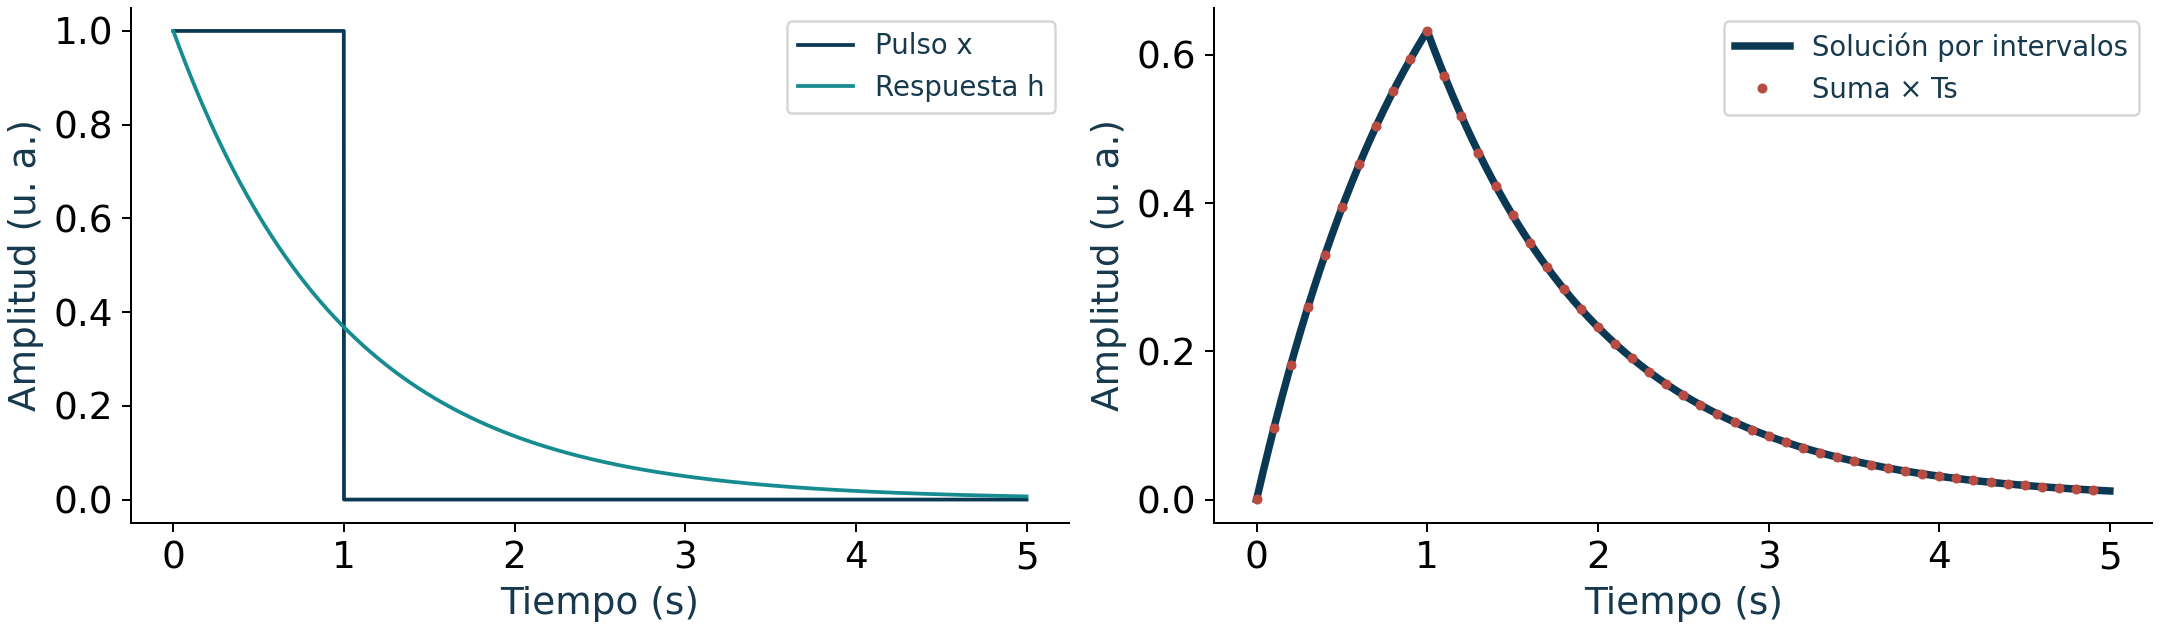
\includegraphics[width=0.95\linewidth,height=\textheight,keepaspectratio]{figuras/convolucion.png}

}

\caption{Ejemplo sintético de la sesión: la suma de convolución se
multiplica por Ts para aproximar la integral.}

\end{figure}%

\note{\textbf{Libro guía:} John Semmlow, \emph{Circuits, Signals, and
Systems for Bioengineers}, 3.ª ed., 2018.

§5.4, \textbf{Using The Impulse Response To Find A Systems Output To Any
Input---Convolution} (página 219 del visor PDF); §5.4.2, \textbf{Matlab
Implementation} (página 229 del visor PDF).

\textbf{Correspondencia:} Ejemplo, figura o implementación de
elaboración docente a partir de estos fundamentos. No es una
transcripción del código MATLAB del libro. Figura de cálculo propio con
señales sintéticas. Código reproducible:
codigo/ejemplos\_verificados.py.

\textbf{Microcurrículo:} semana 11, sesión 1 (sesión global 21). Los
numerales del cronograma son identificadores curriculares; no son los
apartados del libro citados arriba.}
\end{frame}

\begin{frame}{Verificaciones antes de interpretar}
\phantomsection\label{d3-021}
\begin{itemize}
\tightlist
\item
  La longitud completa es \(N_x+N_h-1\).
\item
  La convolución con un impulso reproduce la señal.
\item
  La suma de la salida cumple \(\sum y=(\sum x)(\sum h)\) cuando las
  sumas existen.
\end{itemize}

\note{\textbf{Libro guía:} John Semmlow, \emph{Circuits, Signals, and
Systems for Bioengineers}, 3.ª ed., 2018.

§5.4, \textbf{Using The Impulse Response To Find A Systems Output To Any
Input---Convolution} (página 219 del visor PDF).

\textbf{Correspondencia:} El tema se desarrolla en las secciones
indicadas. La redacción es una síntesis docente.

\textbf{Microcurrículo:} semana 11, sesión 1 (sesión global 21). Los
numerales del cronograma son identificadores curriculares; no son los
apartados del libro citados arriba.}
\end{frame}

\begin{frame}[fragile]{Errores frecuentes}
\phantomsection\label{d3-022}
\begin{itemize}
\tightlist
\item
  Confundir convolución con multiplicación muestra a muestra.
\item
  Olvidar la inversión de \(h[k]\) antes del desplazamiento.
\item
  Comparar resultados \texttt{same} y \texttt{full} sin declarar el
  modo.
\end{itemize}

\note{\textbf{Libro guía:} John Semmlow, \emph{Circuits, Signals, and
Systems for Bioengineers}, 3.ª ed., 2018.

§5.4, \textbf{Using The Impulse Response To Find A Systems Output To Any
Input---Convolution} (página 219 del visor PDF).

\textbf{Correspondencia:} El tema se desarrolla en las secciones
indicadas. La redacción es una síntesis docente.

\textbf{Microcurrículo:} semana 11, sesión 1 (sesión global 21). Los
numerales del cronograma son identificadores curriculares; no son los
apartados del libro citados arriba.}
\end{frame}

\begin{frame}{Actividad guiada}
\phantomsection\label{d3-023}
\begin{enumerate}
\tightlist
\item
  Calcule \([1,2,1]*[1,-1]\).
\item
  Marque qué muestras dependen de condiciones de borde.
\item
  Interprete el segundo núcleo como diferenciador simple.
\end{enumerate}

\textbf{Producto:} cálculo, figura rotulada y explicación de máximo 120
palabras.

\note{\textbf{Libro guía:} John Semmlow, \emph{Circuits, Signals, and
Systems for Bioengineers}, 3.ª ed., 2018.

§5.4, \textbf{Using The Impulse Response To Find A Systems Output To Any
Input---Convolution} (página 219 del visor PDF).

\textbf{Correspondencia:} El tema se desarrolla en las secciones
indicadas. La redacción es una síntesis docente.

\textbf{Microcurrículo:} semana 11, sesión 1 (sesión global 21). Los
numerales del cronograma son identificadores curriculares; no son los
apartados del libro citados arriba.}
\end{frame}

\begin{frame}{Pregunta de comprobación}
\phantomsection\label{d3-024}
Para \(x=[1,2,1]\) y \(h=[1,-1]\), explique por qué la salida tiene
cuatro muestras y verifique su suma.

\begin{block}{Comprobación}

\textbf{Evidencia esperada:} Soporte, valores muestra a muestra y
propiedad de la suma.

\end{block}

\note{\textbf{Libro guía:} John Semmlow, \emph{Circuits, Signals, and
Systems for Bioengineers}, 3.ª ed., 2018.

§5.4, \textbf{Using The Impulse Response To Find A Systems Output To Any
Input---Convolution} (página 219 del visor PDF).

\textbf{Correspondencia:} El tema se desarrolla en las secciones
indicadas. La redacción es una síntesis docente.

\textbf{Microcurrículo:} semana 11, sesión 1 (sesión global 21). Los
numerales del cronograma son identificadores curriculares; no son los
apartados del libro citados arriba.}
\end{frame}

\begin{frame}{Síntesis de la sesión}
\phantomsection\label{d3-025}
\begin{itemize}
\tightlist
\item
  La convolución construye la respuesta de cualquier sistema LTI.
\item
  El soporte anticipa la duración de la salida.
\item
  Los bordes forman parte del modelo computacional.
\end{itemize}

\begin{block}{Criterio de dominio}

Soporte, valores muestra a muestra y propiedad de la suma.

\end{block}

\note{\textbf{Libro guía:} John Semmlow, \emph{Circuits, Signals, and
Systems for Bioengineers}, 3.ª ed., 2018.

§5.4, \textbf{Using The Impulse Response To Find A Systems Output To Any
Input---Convolution} (página 219 del visor PDF).

\textbf{Correspondencia:} El tema se desarrolla en las secciones
indicadas. La redacción es una síntesis docente.

\textbf{Microcurrículo:} semana 11, sesión 1 (sesión global 21). Los
numerales del cronograma son identificadores curriculares; no son los
apartados del libro citados arriba.}
\end{frame}

\begin{frame}{Sesión 22 · Convolución aplicada: suavizado,
diferenciación y promedio móvil}
\phantomsection\label{d3-026}
\begin{block}{Propósito de aprendizaje}

Relacionar la forma del núcleo con el efecto del sistema sobre una
bioseñal.

\end{block}

\note{\textbf{Libro guía:} John Semmlow, \emph{Circuits, Signals, and
Systems for Bioengineers}, 3.ª ed., 2018.

§5.5, \textbf{Applied Convolution---Basic Filters} (página 231 del visor
PDF); §8.5.1, \textbf{Derivative Filters---The Two-Point Central
Difference Algorithm} (página 377 del visor PDF).

\textbf{Correspondencia:} El tema se desarrolla en las secciones
indicadas. La redacción es una síntesis docente.

\textbf{Microcurrículo:} semana 11, sesión 2 (sesión global 22). Los
numerales del cronograma son identificadores curriculares; no son los
apartados del libro citados arriba.}
\end{frame}

\begin{frame}{Preguntas que orientan la sesión}
\phantomsection\label{d3-027}
¿Cuánto retardo añade la ventana elegida? ¿Qué unidad tiene una
diferencia temporal?

\note{\textbf{Libro guía:} John Semmlow, \emph{Circuits, Signals, and
Systems for Bioengineers}, 3.ª ed., 2018.

§5.5, \textbf{Applied Convolution---Basic Filters} (página 231 del visor
PDF); §8.5.1, \textbf{Derivative Filters---The Two-Point Central
Difference Algorithm} (página 377 del visor PDF).

\textbf{Correspondencia:} El tema se desarrolla en las secciones
indicadas. La redacción es una síntesis docente.

\textbf{Microcurrículo:} semana 11, sesión 2 (sesión global 22). Los
numerales del cronograma son identificadores curriculares; no son los
apartados del libro citados arriba.}
\end{frame}

\begin{frame}{Vocabulario mínimo}
\phantomsection\label{d3-028}
\begin{longtable}[]{@{}
  >{\raggedright\arraybackslash}p{(\linewidth - 2\tabcolsep) * \real{0.5000}}
  >{\raggedright\arraybackslash}p{(\linewidth - 2\tabcolsep) * \real{0.5000}}@{}}
\toprule\noalign{}
\begin{minipage}[b]{\linewidth}\raggedright
Concepto
\end{minipage} & \begin{minipage}[b]{\linewidth}\raggedright
Significado operativo
\end{minipage} \\
\midrule\noalign{}
\endhead
\textbf{Promedio móvil} & Núcleo FIR que reduce fluctuaciones
rápidas. \\
\textbf{Diferenciador} & Resalta cambios entre muestras vecinas. \\
\textbf{Ganancia DC} & \(H(0)=\sum h[n]\) mide la respuesta a una
constante. \\
\textbf{Retardo de grupo} & \(-d\arg H(e^{j\Omega})/d\Omega\), en
muestras. \\
\bottomrule\noalign{}
\end{longtable}

\note{\textbf{Libro guía:} John Semmlow, \emph{Circuits, Signals, and
Systems for Bioengineers}, 3.ª ed., 2018.

§5.5, \textbf{Applied Convolution---Basic Filters} (página 231 del visor
PDF); §8.5.1, \textbf{Derivative Filters---The Two-Point Central
Difference Algorithm} (página 377 del visor PDF).

\textbf{Correspondencia:} El tema se desarrolla en las secciones
indicadas. La redacción es una síntesis docente.

\textbf{Microcurrículo:} semana 11, sesión 2 (sesión global 22). Los
numerales del cronograma son identificadores curriculares; no son los
apartados del libro citados arriba.}
\end{frame}

\begin{frame}{Relaciones matemáticas centrales}
\phantomsection\label{d3-029}
\[h_M[n]=\frac{1}{M},\quad 0\le n<M\]

\[y[n]=\frac{1}{M}\sum_{k=0}^{M-1}x[n-k]\]

\[h_d[n]=\delta[n]-\delta[n-1]\quad\Rightarrow\quad y[n]=x[n]-x[n-1]\]

\begin{block}{Lectura de las ecuaciones}

La diferencia conserva unidades de \(x\). Para aproximar \(dx/dt\),
divida por \(T_s\): \(\dot x[n]\approx f_s(x[n]-x[n-1])\). El promedio
móvil causal tiene retardo \((M-1)/2\) muestras donde la fase está
definida.

\end{block}

\note{\textbf{Libro guía:} John Semmlow, \emph{Circuits, Signals, and
Systems for Bioengineers}, 3.ª ed., 2018.

§5.5, \textbf{Applied Convolution---Basic Filters} (página 231 del visor
PDF); §8.5.1, \textbf{Derivative Filters---The Two-Point Central
Difference Algorithm} (página 377 del visor PDF).

\textbf{Correspondencia:} El tema se desarrolla en las secciones
indicadas. La redacción es una síntesis docente.

\textbf{Microcurrículo:} semana 11, sesión 2 (sesión global 22). Los
numerales del cronograma son identificadores curriculares; no son los
apartados del libro citados arriba.}
\end{frame}

\begin{frame}{Procedimiento de análisis}
\phantomsection\label{d3-030}
\begin{enumerate}
\tightlist
\item
  Definir el objetivo fisiológico.
\item
  Convertir la escala temporal a número de muestras.
\item
  Revisar ganancia, retardo y bordes.
\item
  Comparar la salida con eventos anotados.
\end{enumerate}

\begin{block}{Criterio de calidad}

Conversión a milisegundos, ganancia DC y transitorio de inicialización.

\end{block}

\note{\textbf{Libro guía:} John Semmlow, \emph{Circuits, Signals, and
Systems for Bioengineers}, 3.ª ed., 2018.

§5.5, \textbf{Applied Convolution---Basic Filters} (página 231 del visor
PDF); §8.5.1, \textbf{Derivative Filters---The Two-Point Central
Difference Algorithm} (página 377 del visor PDF).

\textbf{Correspondencia:} El tema se desarrolla en las secciones
indicadas. La redacción es una síntesis docente.

\textbf{Microcurrículo:} semana 11, sesión 2 (sesión global 22). Los
numerales del cronograma son identificadores curriculares; no son los
apartados del libro citados arriba.}
\end{frame}

\begin{frame}{Ejemplo biomédico}
\phantomsection\label{d3-031}
Para una envolvente EMG muestreada a 1000 Hz, una ventana de 100 ms
contiene 100 muestras. El promedio reduce variabilidad rápida, aunque
puede desplazar el inicio aparente de activación.

\begin{alertblock}{Alcance}

El ejemplo ilustra procesamiento de señales. No establece por sí mismo
una interpretación diagnóstica.

\end{alertblock}

\note{\textbf{Libro guía:} John Semmlow, \emph{Circuits, Signals, and
Systems for Bioengineers}, 3.ª ed., 2018.

§5.5, \textbf{Applied Convolution---Basic Filters} (página 231 del visor
PDF).

\textbf{Correspondencia:} Actividad o interpretación biomédica de
elaboración docente apoyada en las secciones indicadas.

\textbf{Microcurrículo:} semana 11, sesión 2 (sesión global 22). Los
numerales del cronograma son identificadores curriculares; no son los
apartados del libro citados arriba.}
\end{frame}

\begin{frame}[fragile]{Implementación mínima en Python}
\phantomsection\label{d3-032}
\begin{Shaded}
\begin{Highlighting}[]
\ImportTok{import}\NormalTok{ numpy }\ImportTok{as}\NormalTok{ np}
\ImportTok{from}\NormalTok{ scipy.signal }\ImportTok{import}\NormalTok{ lfilter}
\NormalTok{fs }\OperatorTok{=} \DecValTok{1000}
\NormalTok{M }\OperatorTok{=} \BuiltInTok{round}\NormalTok{(}\FloatTok{0.100} \OperatorTok{*}\NormalTok{ fs)}
\NormalTok{h }\OperatorTok{=}\NormalTok{ np.ones(M) }\OperatorTok{/}\NormalTok{ M}
\NormalTok{y }\OperatorTok{=}\NormalTok{ lfilter(h, [}\FloatTok{1.0}\NormalTok{], x)  }\CommentTok{\# causal, estado inicial cero}
\end{Highlighting}
\end{Shaded}

\note{\textbf{Libro guía:} John Semmlow, \emph{Circuits, Signals, and
Systems for Bioengineers}, 3.ª ed., 2018.

§5.5, \textbf{Applied Convolution---Basic Filters} (página 231 del visor
PDF).

\textbf{Correspondencia:} Ejemplo, figura o implementación de
elaboración docente a partir de estos fundamentos. No es una
transcripción del código MATLAB del libro.

\textbf{Microcurrículo:} semana 11, sesión 2 (sesión global 22). Los
numerales del cronograma son identificadores curriculares; no son los
apartados del libro citados arriba.}
\end{frame}

\begin{frame}{Verificaciones antes de interpretar}
\phantomsection\label{d3-033}
\begin{itemize}
\tightlist
\item
  La suma del promedio móvil debe valer uno.
\item
  Una entrada constante conserva su nivel después del transitorio
  inicial, bajo extensión compatible.
\item
  El retardo de grupo en las bandas de fase definida es \((M-1)/2\)
  muestras.
\end{itemize}

\note{\textbf{Libro guía:} John Semmlow, \emph{Circuits, Signals, and
Systems for Bioengineers}, 3.ª ed., 2018.

§5.5, \textbf{Applied Convolution---Basic Filters} (página 231 del visor
PDF); §8.5.1, \textbf{Derivative Filters---The Two-Point Central
Difference Algorithm} (página 377 del visor PDF).

\textbf{Correspondencia:} El tema se desarrolla en las secciones
indicadas. La redacción es una síntesis docente.

\textbf{Microcurrículo:} semana 11, sesión 2 (sesión global 22). Los
numerales del cronograma son identificadores curriculares; no son los
apartados del libro citados arriba.}
\end{frame}

\begin{frame}{Errores frecuentes}
\phantomsection\label{d3-034}
\begin{itemize}
\tightlist
\item
  Elegir \(M\) sin convertir milisegundos a muestras.
\item
  Interpretar el suavizado como eliminación completa del ruido.
\item
  Usar diferencias sin revisar la amplificación de ruido.
\end{itemize}

\note{\textbf{Libro guía:} John Semmlow, \emph{Circuits, Signals, and
Systems for Bioengineers}, 3.ª ed., 2018.

§5.5, \textbf{Applied Convolution---Basic Filters} (página 231 del visor
PDF); §8.5.1, \textbf{Derivative Filters---The Two-Point Central
Difference Algorithm} (página 377 del visor PDF).

\textbf{Correspondencia:} El tema se desarrolla en las secciones
indicadas. La redacción es una síntesis docente.

\textbf{Microcurrículo:} semana 11, sesión 2 (sesión global 22). Los
numerales del cronograma son identificadores curriculares; no son los
apartados del libro citados arriba.}
\end{frame}

\begin{frame}{Actividad guiada}
\phantomsection\label{d3-035}
\begin{enumerate}
\tightlist
\item
  Compare ventanas de 20, 100 y 250 ms.
\item
  Mida cuánto cambia el tiempo del máximo.
\item
  Explique cuál ventana conserva mejor una activación breve.
\end{enumerate}

\textbf{Producto:} cálculo, figura rotulada y explicación de máximo 120
palabras.

\note{\textbf{Libro guía:} John Semmlow, \emph{Circuits, Signals, and
Systems for Bioengineers}, 3.ª ed., 2018.

§5.5, \textbf{Applied Convolution---Basic Filters} (página 231 del visor
PDF); §8.5.1, \textbf{Derivative Filters---The Two-Point Central
Difference Algorithm} (página 377 del visor PDF).

\textbf{Correspondencia:} El tema se desarrolla en las secciones
indicadas. La redacción es una síntesis docente.

\textbf{Microcurrículo:} semana 11, sesión 2 (sesión global 22). Los
numerales del cronograma son identificadores curriculares; no son los
apartados del libro citados arriba.}
\end{frame}

\begin{frame}{Pregunta de comprobación}
\phantomsection\label{d3-036}
Con \(M=101\) y \(f_s=1000\) Hz, obtenga el retardo y explique qué
ocurre en las primeras \(M-1\) muestras.

\begin{block}{Comprobación}

\textbf{Evidencia esperada:} Conversión a milisegundos, ganancia DC y
transitorio de inicialización.

\end{block}

\note{\textbf{Libro guía:} John Semmlow, \emph{Circuits, Signals, and
Systems for Bioengineers}, 3.ª ed., 2018.

§5.5, \textbf{Applied Convolution---Basic Filters} (página 231 del visor
PDF); §8.5.1, \textbf{Derivative Filters---The Two-Point Central
Difference Algorithm} (página 377 del visor PDF).

\textbf{Correspondencia:} El tema se desarrolla en las secciones
indicadas. La redacción es una síntesis docente.

\textbf{Microcurrículo:} semana 11, sesión 2 (sesión global 22). Los
numerales del cronograma son identificadores curriculares; no son los
apartados del libro citados arriba.}
\end{frame}

\begin{frame}{Síntesis de la sesión}
\phantomsection\label{d3-037}
\begin{itemize}
\tightlist
\item
  El núcleo codifica el comportamiento del filtro.
\item
  Suavizado y resolución temporal compiten.
\item
  La validación debe conservar variables fisiológicas relevantes.
\end{itemize}

\begin{block}{Criterio de dominio}

Conversión a milisegundos, ganancia DC y transitorio de inicialización.

\end{block}

\note{\textbf{Libro guía:} John Semmlow, \emph{Circuits, Signals, and
Systems for Bioengineers}, 3.ª ed., 2018.

§5.5, \textbf{Applied Convolution---Basic Filters} (página 231 del visor
PDF); §8.5.1, \textbf{Derivative Filters---The Two-Point Central
Difference Algorithm} (página 377 del visor PDF).

\textbf{Correspondencia:} El tema se desarrolla en las secciones
indicadas. La redacción es una síntesis docente.

\textbf{Microcurrículo:} semana 11, sesión 2 (sesión global 22). Los
numerales del cronograma son identificadores curriculares; no son los
apartados del libro citados arriba.}
\end{frame}

\begin{frame}{Semana 12 · Respuesta frecuencial y transformada de
Laplace}
\phantomsection\label{d3-038}
\note{\textbf{Libro guía:} John Semmlow, \emph{Circuits, Signals, and
Systems for Bioengineers}, 3.ª ed., 2018.

§5.4, \textbf{Using The Impulse Response To Find A Systems Output To Any
Input---Convolution} (página 219 del visor PDF); §6.4, \textbf{The
Transfer Function} (página 255 del visor PDF); §7.4, \textbf{Nonzero
Initial Conditions---Initial And Final Value Theorems} (página 326 del
visor PDF); §8.4, \textbf{Linear Filters---Introduction} (página 358 del
visor PDF).

\textbf{Correspondencia:} Síntesis o encuadre que reúne varias
secciones; no corresponde a un único apartado del libro.

\textbf{Lectura:} use estas secciones como ruta de preparación y
consulta. La bibliografía aparece al final del bloque.}
\end{frame}

\begin{frame}{Sesión 23 · Convolución en frecuencia y respuesta del
sistema}
\phantomsection\label{d3-039}
\begin{block}{Propósito de aprendizaje}

Usar la función de transferencia frecuencial para predecir amplitud y
fase de la salida.

\end{block}

\note{\textbf{Libro guía:} John Semmlow, \emph{Circuits, Signals, and
Systems for Bioengineers}, 3.ª ed., 2018.

§5.6, \textbf{Convolution In The Frequency Domain} (página 237 del visor
PDF); §6.4, \textbf{The Transfer Function} (página 255 del visor PDF);
§6.7, \textbf{The Transfer Function And The Fourier Transform} (página
287 del visor PDF).

\textbf{Correspondencia:} El tema se desarrolla en las secciones
indicadas. La redacción es una síntesis docente.

\textbf{Microcurrículo:} semana 12, sesión 1 (sesión global 23). Los
numerales del cronograma son identificadores curriculares; no son los
apartados del libro citados arriba.}
\end{frame}

\begin{frame}{Preguntas que orientan la sesión}
\phantomsection\label{d3-040}
¿Qué frecuencia atenúa el sistema? ¿La fase conserva la forma de la
señal?

\note{\textbf{Libro guía:} John Semmlow, \emph{Circuits, Signals, and
Systems for Bioengineers}, 3.ª ed., 2018.

§5.6, \textbf{Convolution In The Frequency Domain} (página 237 del visor
PDF); §6.4, \textbf{The Transfer Function} (página 255 del visor PDF);
§6.7, \textbf{The Transfer Function And The Fourier Transform} (página
287 del visor PDF).

\textbf{Correspondencia:} El tema se desarrolla en las secciones
indicadas. La redacción es una síntesis docente.

\textbf{Microcurrículo:} semana 12, sesión 1 (sesión global 23). Los
numerales del cronograma son identificadores curriculares; no son los
apartados del libro citados arriba.}
\end{frame}

\begin{frame}{Vocabulario mínimo}
\phantomsection\label{d3-041}
\begin{longtable}[]{@{}
  >{\raggedright\arraybackslash}p{(\linewidth - 2\tabcolsep) * \real{0.5000}}
  >{\raggedright\arraybackslash}p{(\linewidth - 2\tabcolsep) * \real{0.5000}}@{}}
\toprule\noalign{}
\begin{minipage}[b]{\linewidth}\raggedright
Concepto
\end{minipage} & \begin{minipage}[b]{\linewidth}\raggedright
Significado operativo
\end{minipage} \\
\midrule\noalign{}
\endhead
\textbf{Respuesta frecuencial} & \(H(e^{j\Omega})\) describe la acción
sobre cada frecuencia. \\
\textbf{Magnitud} & Indica cuánto amplifica o atenúa. \\
\textbf{Fase} & Determina el desplazamiento relativo de componentes. \\
\textbf{Convolución} & En tiempo equivale a multiplicación en
frecuencia. \\
\bottomrule\noalign{}
\end{longtable}

\note{\textbf{Libro guía:} John Semmlow, \emph{Circuits, Signals, and
Systems for Bioengineers}, 3.ª ed., 2018.

§6.4, \textbf{The Transfer Function} (página 255 del visor PDF); §8.2.3,
\textbf{Transformation From The Z-Domain To The Frequency Domain}
(página 353 del visor PDF).

\textbf{Correspondencia:} El tema se desarrolla en las secciones
indicadas. La redacción es una síntesis docente.

\textbf{Microcurrículo:} semana 12, sesión 1 (sesión global 23). Los
numerales del cronograma son identificadores curriculares; no son los
apartados del libro citados arriba.}
\end{frame}

\begin{frame}{Relaciones matemáticas centrales}
\phantomsection\label{d3-042}
\[y[n]=x[n]*h[n]\Longleftrightarrow Y(e^{j\Omega})=X(e^{j\Omega})H(e^{j\Omega})\]

\[|Y|=|X||H|\]

\[\angle Y=\angle X+\angle H\]

\begin{block}{Lectura de las ecuaciones}

Para respuesta de estado cero, un LTI no crea frecuencias nuevas. Solo
los ceros situados en el eje de evaluación (\(j\omega\) o círculo
unitario) anulan una frecuencia real exacta.

\end{block}

\note{\textbf{Libro guía:} John Semmlow, \emph{Circuits, Signals, and
Systems for Bioengineers}, 3.ª ed., 2018.

§5.6, \textbf{Convolution In The Frequency Domain} (página 237 del visor
PDF); §6.4, \textbf{The Transfer Function} (página 255 del visor PDF);
§6.7, \textbf{The Transfer Function And The Fourier Transform} (página
287 del visor PDF).

\textbf{Correspondencia:} El tema se desarrolla en las secciones
indicadas. La redacción es una síntesis docente.

\textbf{Microcurrículo:} semana 12, sesión 1 (sesión global 23). Los
numerales del cronograma son identificadores curriculares; no son los
apartados del libro citados arriba.}
\end{frame}

\begin{frame}{Modelos de sistemas y conexiones}
\phantomsection\label{d3-043}
Para sistemas lineales compatibles y respuesta de estado cero:

\begin{longtable}[]{@{}ll@{}}
\toprule\noalign{}
Conexión & Transferencia equivalente \\
\midrule\noalign{}
\endhead
Cascada & \(H_1H_2\) \\
Paralelo & \(H_1+H_2\) \\
Realimentación negativa & \(G/(1+GF)\) \\
\bottomrule\noalign{}
\end{longtable}

\begin{block}{Concepto clave}

En realimentación, \(G\) describe la trayectoria directa y \(F\) la
medición de retorno. La estructura y el signo determinan la ecuación
característica. Debe comprobarse estabilidad de la conexión.

\end{block}

\textbf{Aplicación:} un modelo de regulación pupilar distingue estímulo,
salida medida y mecanismo de realimentación.

\note{\textbf{Libro guía:} John Semmlow, \emph{Circuits, Signals, and
Systems for Bioengineers}, 3.ª ed., 2018.

§6.2, \textbf{Systems Analysis Models} (página 248 del visor PDF);
§1.4.5, \textbf{Biosystems Modeling} (página 46 del visor PDF).

\textbf{Correspondencia:} El tema se desarrolla en las secciones
indicadas. La redacción es una síntesis docente.

\textbf{Microcurrículo:} semana 12, sesión 1 (sesión global 23). Los
numerales del cronograma son identificadores curriculares; no son los
apartados del libro citados arriba.}
\end{frame}

\begin{frame}{Respuesta sinusoidal y fasores}
\phantomsection\label{d3-044}
Para una entrada \(x(t)=A\cos(\omega t+\phi)\) y un LTI estable:

\[y_{ss}(t)=A|H(j\omega)|\cos\big(\omega t+\phi+\arg H(j\omega)\big).\]

El fasor de entrada es \(\tilde X=Ae^{j\phi}\) y
\(\tilde Y=H(j\omega)\tilde X\).

\begin{block}{Concepto clave}

Esta expresión describe régimen permanente. La respuesta total puede
incluir un transitorio debido al inicio de la excitación o a condiciones
iniciales.

\end{block}

\note{\textbf{Libro guía:} John Semmlow, \emph{Circuits, Signals, and
Systems for Bioengineers}, 3.ª ed., 2018.

§6.3, \textbf{The Response Of System Elements To Sinusoidal Inputs:
Phasor Analysis} (página 251 del visor PDF); §6.4, \textbf{The Transfer
Function} (página 255 del visor PDF).

\textbf{Correspondencia:} El tema se desarrolla en las secciones
indicadas. La redacción es una síntesis docente.

\textbf{Microcurrículo:} semana 12, sesión 1 (sesión global 23). Los
numerales del cronograma son identificadores curriculares; no son los
apartados del libro citados arriba.}
\end{frame}

\begin{frame}{Bode de un sistema de primer orden}
\phantomsection\label{d3-045}
Para \(H(j\omega)=K/(1+j\omega\tau)\), con \(K>0\):

\[|H|=\frac{K}{\sqrt{1+(\omega\tau)^2}},\qquad
\arg H=-\arctan(\omega\tau).\]

\begin{itemize}
\tightlist
\item
  Frecuencia de corte: \(f_c=1/(2\pi\tau)\).
\item
  En \(f_c\): magnitud \(K/\sqrt2\) y fase \(-45^\circ\).
\item
  Para \(f\gg f_c\): pendiente aproximada de \(-20\) dB/década.
\end{itemize}

\begin{block}{Nota}

Para una transferencia con unidades físicas, los dB requieren una
referencia de ganancia con las mismas unidades. Aquí se supone entrada y
salida de la misma magnitud.

\end{block}

\note{\textbf{Libro guía:} John Semmlow, \emph{Circuits, Signals, and
Systems for Bioengineers}, 3.ª ed., 2018.

§6.5.4, \textbf{First-Order Element} (página 266 del visor PDF).

\textbf{Correspondencia:} El tema se desarrolla en las secciones
indicadas. La redacción es una síntesis docente.

\textbf{Microcurrículo:} semana 12, sesión 1 (sesión global 23). Los
numerales del cronograma son identificadores curriculares; no son los
apartados del libro citados arriba.}
\end{frame}

\begin{frame}{Magnitud y fase de un primer orden}
\phantomsection\label{d3-046}
\begin{figure}[H]

{\centering 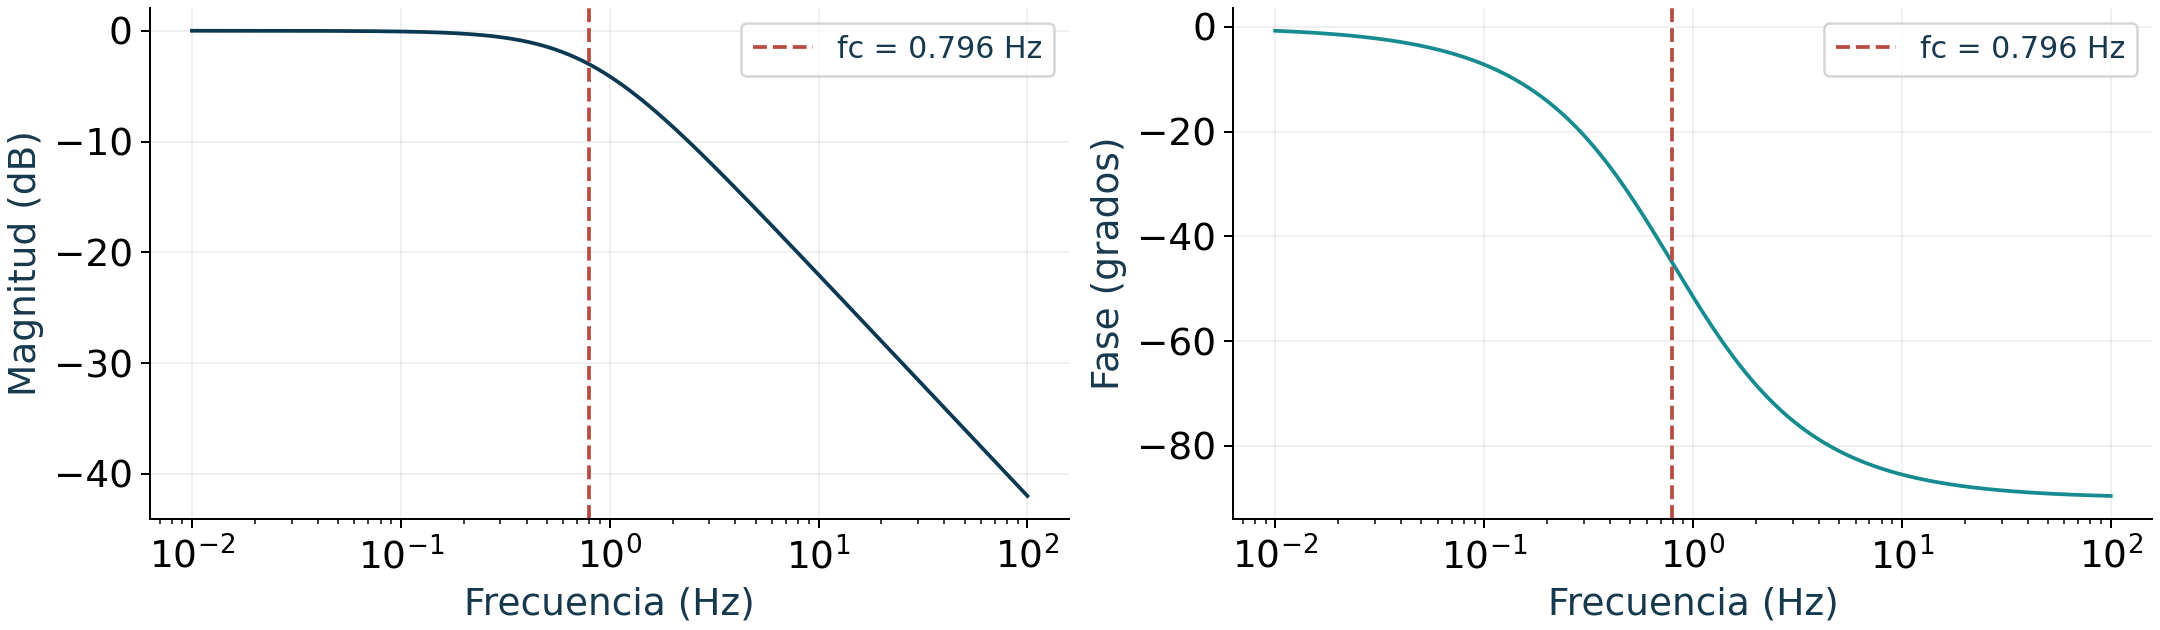
\includegraphics[width=0.95\linewidth,height=\textheight,keepaspectratio]{figuras/bode-primer-orden.png}

}

\caption{Simulación con K = 1 y constante de tiempo de 0.2 s. La línea
vertical señala la frecuencia de corte, aproximadamente 0.796 Hz.}

\end{figure}%

\note{\textbf{Libro guía:} John Semmlow, \emph{Circuits, Signals, and
Systems for Bioengineers}, 3.ª ed., 2018.

§6.5.4, \textbf{First-Order Element} (página 266 del visor PDF).

\textbf{Correspondencia:} Ejemplo, figura o implementación de
elaboración docente a partir de estos fundamentos. No es una
transcripción del código MATLAB del libro. Figura de cálculo propio con
señales sintéticas. Código reproducible:
codigo/ejemplos\_verificados.py.

\textbf{Microcurrículo:} semana 12, sesión 1 (sesión global 23). Los
numerales del cronograma son identificadores curriculares; no son los
apartados del libro citados arriba.}
\end{frame}

\begin{frame}{Segundo orden, amortiguamiento y resonancia}
\phantomsection\label{d3-047}
\[H(s)=\frac{K\omega_n^2}{s^2+2\zeta\omega_ns+\omega_n^2}.\]

Para \(0<\zeta<1\):

\[p_{1,2}=-\zeta\omega_n\pm j\omega_n\sqrt{1-\zeta^2}.\]

\begin{block}{Concepto clave}

La frecuencia natural \(\omega_n\) y la frecuencia de oscilación
amortiguada son distintas. En este pasa bajas de segundo orden aparece
pico resonante cuando \(\zeta<1/\sqrt2\).

\end{block}

Un modo poco amortiguado puede producir oscilaciones posteriores a un
transitorio. No atribuya esas oscilaciones al organismo sin revisar la
dinámica instrumental.

\note{\textbf{Libro guía:} John Semmlow, \emph{Circuits, Signals, and
Systems for Bioengineers}, 3.ª ed., 2018.

§6.5.5, \textbf{Second-Order Element} (página 271 del visor PDF);
§7.3.6, \textbf{Second-Order Element} (página 314 del visor PDF).

\textbf{Correspondencia:} El tema se desarrolla en las secciones
indicadas. La redacción es una síntesis docente.

\textbf{Microcurrículo:} semana 12, sesión 1 (sesión global 23). Los
numerales del cronograma son identificadores curriculares; no son los
apartados del libro citados arriba.}
\end{frame}

\begin{frame}{Composición de Bode y reconocimiento de dinámica}
\phantomsection\label{d3-048}
En cascada, \(H=H_1H_2\):

\[20\log_{10}|H|=20\log_{10}|H_1|+20\log_{10}|H_2|,\]
\[\arg H=\arg H_1+\arg H_2\quad(\bmod\ 2\pi).\]

\begin{longtable}[]{@{}ll@{}}
\toprule\noalign{}
Elemento & Pendiente asintótica de magnitud \\
\midrule\noalign{}
\endhead
Ganancia constante & 0 dB/década \\
Integrador & \(-20\) dB/década \\
Diferenciador & \(+20\) dB/década \\
Polo real de primer orden & cambio de \(-20\) dB/década \\
\bottomrule\noalign{}
\end{longtable}

Las pendientes orientan la identificación, pero no prueban un modelo
único. El ruido y la banda de excitación limitan la inferencia.

\note{\textbf{Libro guía:} John Semmlow, \emph{Circuits, Signals, and
Systems for Bioengineers}, 3.ª ed., 2018.

§6.5.1, \textbf{Constant Gain Element} (página 264 del visor PDF);
§6.5.2, \textbf{Derivative Element} (página 264 del visor PDF); §6.5.3,
\textbf{Integrator Element} (página 266 del visor PDF); §6.6,
\textbf{Bode Plots Combining Multiple Elements} (página 277 del visor
PDF); §6.6.1, \textbf{Constructing The Transfer Function From The System
Spectrum} (página 286 del visor PDF).

\textbf{Correspondencia:} El tema se desarrolla en las secciones
indicadas. La redacción es una síntesis docente.

\textbf{Microcurrículo:} semana 12, sesión 1 (sesión global 23). Los
numerales del cronograma son identificadores curriculares; no son los
apartados del libro citados arriba.}
\end{frame}

\begin{frame}{Procedimiento de análisis}
\phantomsection\label{d3-049}
\begin{enumerate}
\tightlist
\item
  Estimar o calcular \(H\).
\item
  Examinar magnitud en la banda fisiológica.
\item
  Revisar fase o retardo de grupo.
\item
  Predecir distorsión antes de filtrar.
\end{enumerate}

\begin{block}{Criterio de calidad}

Magnitud, decibelios, fase y conexión con la frecuencia de corte.

\end{block}

\note{\textbf{Libro guía:} John Semmlow, \emph{Circuits, Signals, and
Systems for Bioengineers}, 3.ª ed., 2018.

§5.6, \textbf{Convolution In The Frequency Domain} (página 237 del visor
PDF); §6.4, \textbf{The Transfer Function} (página 255 del visor PDF);
§6.7, \textbf{The Transfer Function And The Fourier Transform} (página
287 del visor PDF).

\textbf{Correspondencia:} El tema se desarrolla en las secciones
indicadas. La redacción es una síntesis docente.

\textbf{Microcurrículo:} semana 12, sesión 1 (sesión global 23). Los
numerales del cronograma son identificadores curriculares; no son los
apartados del libro citados arriba.}
\end{frame}

\begin{frame}{Ejemplo biomédico}
\phantomsection\label{d3-050}
Un suavizador aplicado a ECG puede atenuar interferencia rápida, pero
también reducir la pendiente del QRS si su banda de paso es
insuficiente.

\begin{alertblock}{Alcance}

El ejemplo ilustra procesamiento de señales. No establece por sí mismo
una interpretación diagnóstica.

\end{alertblock}

\note{\textbf{Libro guía:} John Semmlow, \emph{Circuits, Signals, and
Systems for Bioengineers}, 3.ª ed., 2018.

§5.6, \textbf{Convolution In The Frequency Domain} (página 237 del visor
PDF); §6.4, \textbf{The Transfer Function} (página 255 del visor PDF);
§6.7, \textbf{The Transfer Function And The Fourier Transform} (página
287 del visor PDF).

\textbf{Correspondencia:} El tema se desarrolla en las secciones
indicadas. La redacción es una síntesis docente.

\textbf{Microcurrículo:} semana 12, sesión 1 (sesión global 23). Los
numerales del cronograma son identificadores curriculares; no son los
apartados del libro citados arriba.}
\end{frame}

\begin{frame}[fragile]{Implementación mínima en Python}
\phantomsection\label{d3-051}
\begin{Shaded}
\begin{Highlighting}[]
\ImportTok{import}\NormalTok{ numpy }\ImportTok{as}\NormalTok{ np}
\ImportTok{from}\NormalTok{ scipy.signal }\ImportTok{import}\NormalTok{ freqz}
\NormalTok{h }\OperatorTok{=}\NormalTok{ np.ones(}\DecValTok{11}\NormalTok{) }\OperatorTok{/} \DecValTok{11}
\NormalTok{f, H }\OperatorTok{=}\NormalTok{ freqz(h, worN}\OperatorTok{=}\DecValTok{2048}\NormalTok{, fs}\OperatorTok{=}\DecValTok{500}\NormalTok{)}
\NormalTok{mag\_db }\OperatorTok{=} \DecValTok{20}\OperatorTok{*}\NormalTok{np.log10(np.maximum(np.}\BuiltInTok{abs}\NormalTok{(H), }\FloatTok{1e{-}12}\NormalTok{))}
\end{Highlighting}
\end{Shaded}

\note{\textbf{Libro guía:} John Semmlow, \emph{Circuits, Signals, and
Systems for Bioengineers}, 3.ª ed., 2018.

§8.4.1, \textbf{Filter Properties} (página 360 del visor PDF).

\textbf{Correspondencia:} Ejemplo, figura o implementación de
elaboración docente a partir de estos fundamentos. No es una
transcripción del código MATLAB del libro.

\textbf{Microcurrículo:} semana 12, sesión 1 (sesión global 23). Los
numerales del cronograma son identificadores curriculares; no son los
apartados del libro citados arriba.}
\end{frame}

\begin{frame}{Verificaciones antes de interpretar}
\phantomsection\label{d3-052}
\begin{itemize}
\tightlist
\item
  \(H(0)\) coincide con la suma de coeficientes.
\item
  Una convolución temporal y una multiplicación FFT deben concordar si
  se usa relleno suficiente.
\item
  La fase debe desenvolverse antes de calcular su pendiente.
\end{itemize}

\note{\textbf{Libro guía:} John Semmlow, \emph{Circuits, Signals, and
Systems for Bioengineers}, 3.ª ed., 2018.

§5.6, \textbf{Convolution In The Frequency Domain} (página 237 del visor
PDF); §6.4, \textbf{The Transfer Function} (página 255 del visor PDF);
§6.7, \textbf{The Transfer Function And The Fourier Transform} (página
287 del visor PDF).

\textbf{Correspondencia:} El tema se desarrolla en las secciones
indicadas. La redacción es una síntesis docente.

\textbf{Microcurrículo:} semana 12, sesión 1 (sesión global 23). Los
numerales del cronograma son identificadores curriculares; no son los
apartados del libro citados arriba.}
\end{frame}

\begin{frame}{Errores frecuentes}
\phantomsection\label{d3-053}
\begin{itemize}
\tightlist
\item
  Usar FFT circular cuando se necesita convolución lineal.
\item
  Ignorar la fase porque la magnitud luce adecuada.
\item
  Expresar frecuencia normalizada sin indicar su referencia.
\end{itemize}

\note{\textbf{Libro guía:} John Semmlow, \emph{Circuits, Signals, and
Systems for Bioengineers}, 3.ª ed., 2018.

§5.6, \textbf{Convolution In The Frequency Domain} (página 237 del visor
PDF); §6.4, \textbf{The Transfer Function} (página 255 del visor PDF);
§6.7, \textbf{The Transfer Function And The Fourier Transform} (página
287 del visor PDF).

\textbf{Correspondencia:} El tema se desarrolla en las secciones
indicadas. La redacción es una síntesis docente.

\textbf{Microcurrículo:} semana 12, sesión 1 (sesión global 23). Los
numerales del cronograma son identificadores curriculares; no son los
apartados del libro citados arriba.}
\end{frame}

\begin{frame}{Actividad guiada}
\phantomsection\label{d3-054}
\begin{enumerate}
\tightlist
\item
  Prediga la salida para una suma de 5 y 60 Hz.
\item
  Localice la primera anulación del promedio móvil.
\item
  Explique por qué el relleno evita aliasing circular.
\end{enumerate}

\textbf{Producto:} cálculo, figura rotulada y explicación de máximo 120
palabras.

\note{\textbf{Libro guía:} John Semmlow, \emph{Circuits, Signals, and
Systems for Bioengineers}, 3.ª ed., 2018.

§5.6, \textbf{Convolution In The Frequency Domain} (página 237 del visor
PDF); §6.4, \textbf{The Transfer Function} (página 255 del visor PDF);
§6.7, \textbf{The Transfer Function And The Fourier Transform} (página
287 del visor PDF).

\textbf{Correspondencia:} El tema se desarrolla en las secciones
indicadas. La redacción es una síntesis docente.

\textbf{Microcurrículo:} semana 12, sesión 1 (sesión global 23). Los
numerales del cronograma son identificadores curriculares; no son los
apartados del libro citados arriba.}
\end{frame}

\begin{frame}{Pregunta de comprobación}
\phantomsection\label{d3-055}
Para \(H(j\omega)=1/(1+j\omega\tau)\), evalúe magnitud y fase cuando
\(\omega\tau=1\).

\begin{block}{Comprobación}

\textbf{Evidencia esperada:} Magnitud, decibelios, fase y conexión con
la frecuencia de corte.

\end{block}

\note{\textbf{Libro guía:} John Semmlow, \emph{Circuits, Signals, and
Systems for Bioengineers}, 3.ª ed., 2018.

§5.6, \textbf{Convolution In The Frequency Domain} (página 237 del visor
PDF); §6.4, \textbf{The Transfer Function} (página 255 del visor PDF);
§6.7, \textbf{The Transfer Function And The Fourier Transform} (página
287 del visor PDF).

\textbf{Correspondencia:} El tema se desarrolla en las secciones
indicadas. La redacción es una síntesis docente.

\textbf{Microcurrículo:} semana 12, sesión 1 (sesión global 23). Los
numerales del cronograma son identificadores curriculares; no son los
apartados del libro citados arriba.}
\end{frame}

\begin{frame}{Síntesis de la sesión}
\phantomsection\label{d3-056}
\begin{itemize}
\tightlist
\item
  La función de transferencia resume la acción LTI.
\item
  Magnitud y fase forman una descripción conjunta.
\item
  La banda útil depende de la variable biomédica.
\end{itemize}

\begin{block}{Criterio de dominio}

Magnitud, decibelios, fase y conexión con la frecuencia de corte.

\end{block}

\note{\textbf{Libro guía:} John Semmlow, \emph{Circuits, Signals, and
Systems for Bioengineers}, 3.ª ed., 2018.

§5.6, \textbf{Convolution In The Frequency Domain} (página 237 del visor
PDF); §6.4, \textbf{The Transfer Function} (página 255 del visor PDF);
§6.7, \textbf{The Transfer Function And The Fourier Transform} (página
287 del visor PDF).

\textbf{Correspondencia:} El tema se desarrolla en las secciones
indicadas. La redacción es una síntesis docente.

\textbf{Microcurrículo:} semana 12, sesión 1 (sesión global 23). Los
numerales del cronograma son identificadores curriculares; no son los
apartados del libro citados arriba.}
\end{frame}

\begin{frame}{Sesión 24 · Transformada de Laplace, región de
convergencia y función de transferencia}
\phantomsection\label{d3-057}
\begin{block}{Propósito de aprendizaje}

Representar sistemas continuos mediante polos y ceros, incorporando
causalidad y estabilidad.

\end{block}

\note{\textbf{Libro guía:} John Semmlow, \emph{Circuits, Signals, and
Systems for Bioengineers}, 3.ª ed., 2018.

§7.2, \textbf{The Laplace Transform} (página 299 del visor PDF); §7.3,
\textbf{The Laplace Domain Transfer Function} (página 304 del visor
PDF).

\textbf{Correspondencia:} El tema se desarrolla en las secciones
indicadas. La redacción es una síntesis docente.

\textbf{Microcurrículo:} semana 12, sesión 2 (sesión global 24). Los
numerales del cronograma son identificadores curriculares; no son los
apartados del libro citados arriba.}
\end{frame}

\begin{frame}{Preguntas que orientan la sesión}
\phantomsection\label{d3-058}
¿Qué variable física relaciona la transferencia? ¿Qué ROC corresponde al
sistema causal?

\note{\textbf{Libro guía:} John Semmlow, \emph{Circuits, Signals, and
Systems for Bioengineers}, 3.ª ed., 2018.

§7.2, \textbf{The Laplace Transform} (página 299 del visor PDF); §7.3,
\textbf{The Laplace Domain Transfer Function} (página 304 del visor
PDF).

\textbf{Correspondencia:} El tema se desarrolla en las secciones
indicadas. La redacción es una síntesis docente.

\textbf{Microcurrículo:} semana 12, sesión 2 (sesión global 24). Los
numerales del cronograma son identificadores curriculares; no son los
apartados del libro citados arriba.}
\end{frame}

\begin{frame}{Vocabulario mínimo}
\phantomsection\label{d3-059}
\begin{longtable}[]{@{}
  >{\raggedright\arraybackslash}p{(\linewidth - 2\tabcolsep) * \real{0.5000}}
  >{\raggedright\arraybackslash}p{(\linewidth - 2\tabcolsep) * \real{0.5000}}@{}}
\toprule\noalign{}
\begin{minipage}[b]{\linewidth}\raggedright
Concepto
\end{minipage} & \begin{minipage}[b]{\linewidth}\raggedright
Significado operativo
\end{minipage} \\
\midrule\noalign{}
\endhead
\textbf{Variable compleja} & \(s=\sigma+j\omega\) combina crecimiento y
oscilación. \\
\textbf{ROC} & Valores de \(s\) para los que converge la integral. \\
\textbf{Polo} & Singularidad de la expresión racional irreducible de la
transformada. \\
\textbf{Cero} & Valor donde la transformada se anula. \\
\bottomrule\noalign{}
\end{longtable}

\note{\textbf{Libro guía:} John Semmlow, \emph{Circuits, Signals, and
Systems for Bioengineers}, 3.ª ed., 2018.

§7.2.1, \textbf{Definition Of The Laplace Transform} (página 299 del
visor PDF); §7.3, \textbf{The Laplace Domain Transfer Function} (página
304 del visor PDF).

\textbf{Correspondencia:} Las secciones aportan el fundamento. La
diapositiva amplía la formulación o precisa condiciones que no se
presentan con idéntica notación en el libro.

\textbf{Microcurrículo:} semana 12, sesión 2 (sesión global 24). Los
numerales del cronograma son identificadores curriculares; no son los
apartados del libro citados arriba.}
\end{frame}

\begin{frame}{Relaciones matemáticas centrales}
\phantomsection\label{d3-060}
\[X(s)=\int_{-\infty}^{\infty}x(t)e^{-st}\,dt\]

\[H(s)=\frac{Y(s)}{X(s)}\Big|_{\text{condiciones iniciales nulas}}\]

\[H(s)=K\frac{\prod_m(s-z_m)}{\prod_r(s-p_r)}\]

\begin{block}{Lectura de las ecuaciones}

Polos y ceros no bastan sin la región de convergencia. Una misma
expresión algebraica puede corresponder a señales causales o
anticausales distintas.

\end{block}

\note{\textbf{Libro guía:} John Semmlow, \emph{Circuits, Signals, and
Systems for Bioengineers}, 3.ª ed., 2018.

§7.2.1, \textbf{Definition Of The Laplace Transform} (página 299 del
visor PDF); §7.3, \textbf{The Laplace Domain Transfer Function} (página
304 del visor PDF).

\textbf{Correspondencia:} Las secciones aportan el fundamento. La
diapositiva amplía la formulación o precisa condiciones que no se
presentan con idéntica notación en el libro. La definición bilateral y
la ROC amplían el tratamiento unilateral del libro. Véase la distinción
explícita añadida en esta sesión.

\textbf{Microcurrículo:} semana 12, sesión 2 (sesión global 24). Los
numerales del cronograma son identificadores curriculares; no son los
apartados del libro citados arriba.}
\end{frame}

\begin{frame}{Laplace bilateral y unilateral}
\phantomsection\label{d3-061}
La definición bilateral describe también señales para \(t<0\) y permite
estudiar la ROC.

Para condiciones iniciales se usa la unilateral:

\[X_+(s)=\int_{0^-}^{\infty}x(t)e^{-st}dt,\qquad
\mathcal L_+\{\dot x\}=sX_+(s)-x(0^-).\]

\begin{block}{Concepto clave}

El libro desarrolla principalmente la forma unilateral. La bilateral se
conserva como ampliación para estudiar causalidad y ROC. No transfiera
las fórmulas de condiciones iniciales a una definición bilateral sin
justificarlas.

\end{block}

\note{\textbf{Libro guía:} John Semmlow, \emph{Circuits, Signals, and
Systems for Bioengineers}, 3.ª ed., 2018.

§7.2.1, \textbf{Definition Of The Laplace Transform} (página 299 del
visor PDF); §7.2.2, \textbf{Calculus Operations In The Laplace Domain}
(página 301 del visor PDF); §7.4.1, \textbf{Nonzero Initial Conditions}
(página 326 del visor PDF).

\textbf{Correspondencia:} Las secciones aportan el fundamento. La
diapositiva amplía la formulación o precisa condiciones que no se
presentan con idéntica notación en el libro.

\textbf{Microcurrículo:} semana 12, sesión 2 (sesión global 24). Los
numerales del cronograma son identificadores curriculares; no son los
apartados del libro citados arriba.}
\end{frame}

\begin{frame}{La misma expresión, dos regiones de convergencia}
\phantomsection\label{d3-062}
\[\frac1{s+a}\quad(a>0)\]

\begin{longtable}[]{@{}
  >{\raggedright\arraybackslash}p{(\linewidth - 4\tabcolsep) * \real{0.3333}}
  >{\raggedright\arraybackslash}p{(\linewidth - 4\tabcolsep) * \real{0.3333}}
  >{\raggedright\arraybackslash}p{(\linewidth - 4\tabcolsep) * \real{0.3333}}@{}}
\toprule\noalign{}
\begin{minipage}[b]{\linewidth}\raggedright
Señal bilateral
\end{minipage} & \begin{minipage}[b]{\linewidth}\raggedright
ROC
\end{minipage} & \begin{minipage}[b]{\linewidth}\raggedright
Interpretación
\end{minipage} \\
\midrule\noalign{}
\endhead
\(e^{-at}u(t)\) & \(\Re(s)>-a\) & causal, absolutamente integrable \\
\(-e^{-at}u(-t)\) & \(\Re(s)<-a\) & anticausal, no absolutamente
integrable \\
\bottomrule\noalign{}
\end{longtable}

\begin{block}{Concepto clave}

En el primer caso la ROC incluye el eje \(j\omega\) y existe Fourier
ordinaria. La fracción racional sola no determina soporte ni
estabilidad.

\end{block}

\note{\textbf{Libro guía:} John Semmlow, \emph{Circuits, Signals, and
Systems for Bioengineers}, 3.ª ed., 2018.

§7.2.1, \textbf{Definition Of The Laplace Transform} (página 299 del
visor PDF); §7.2.4, \textbf{Converting The Laplace Transform To The
Frequency Domain} (página 303 del visor PDF); §7.5, \textbf{The Laplace
Domain, The Frequency Domain, And The Time Domain} (página 330 del visor
PDF).

\textbf{Correspondencia:} Las secciones aportan el fundamento. La
diapositiva amplía la formulación o precisa condiciones que no se
presentan con idéntica notación en el libro. La ROC bilateral es una
extensión matemática respecto al tratamiento unilateral del libro.

\textbf{Microcurrículo:} semana 12, sesión 2 (sesión global 24). Los
numerales del cronograma son identificadores curriculares; no son los
apartados del libro citados arriba.}
\end{frame}

\begin{frame}{Procedimiento de análisis}
\phantomsection\label{d3-063}
\begin{enumerate}
\tightlist
\item
  Obtener la ecuación diferencial.
\item
  Aplicar Laplace con condiciones iniciales nulas para \(H(s)\).
\item
  Factorizar numerador y denominador.
\item
  Relacionar polos con modos temporales.
\end{enumerate}

\begin{block}{Criterio de calidad}

Inversa, soporte temporal e inclusión del eje imaginario en la ROC.

\end{block}

\note{\textbf{Libro guía:} John Semmlow, \emph{Circuits, Signals, and
Systems for Bioengineers}, 3.ª ed., 2018.

§7.2, \textbf{The Laplace Transform} (página 299 del visor PDF); §7.3,
\textbf{The Laplace Domain Transfer Function} (página 304 del visor
PDF).

\textbf{Correspondencia:} El tema se desarrolla en las secciones
indicadas. La redacción es una síntesis docente.

\textbf{Microcurrículo:} semana 12, sesión 2 (sesión global 24). Los
numerales del cronograma son identificadores curriculares; no son los
apartados del libro citados arriba.}
\end{frame}

\begin{frame}{Ejemplo biomédico}
\phantomsection\label{d3-064}
Un circuito RC con entrada de voltaje y salida sobre el capacitor tiene
\(H(s)=1/(1+s\tau)\), con \(\tau=RC\). Si una membrana pasiva recibe
corriente \(I\) y se observa voltaje \(V\), entonces
\(V(s)/I(s)=R/(1+sRC)\), en ohmios.

\begin{alertblock}{Alcance}

El ejemplo ilustra procesamiento de señales. No establece por sí mismo
una interpretación diagnóstica.

\end{alertblock}

\note{\textbf{Libro guía:} John Semmlow, \emph{Circuits, Signals, and
Systems for Bioengineers}, 3.ª ed., 2018.

§7.3.5, \textbf{First-Order Element} (página 310 del visor PDF);
§12.6.1, \textbf{Electrical Elements With Zero Initial Conditions}
(página 552 del visor PDF).

\textbf{Correspondencia:} Actividad o interpretación biomédica de
elaboración docente apoyada en las secciones indicadas.

\textbf{Microcurrículo:} semana 12, sesión 2 (sesión global 24). Los
numerales del cronograma son identificadores curriculares; no son los
apartados del libro citados arriba.}
\end{frame}

\begin{frame}[fragile]{Implementación mínima en Python}
\phantomsection\label{d3-065}
\begin{Shaded}
\begin{Highlighting}[]
\ImportTok{import}\NormalTok{ numpy }\ImportTok{as}\NormalTok{ np}
\ImportTok{from}\NormalTok{ scipy.signal }\ImportTok{import}\NormalTok{ TransferFunction, step}
\NormalTok{tau }\OperatorTok{=} \FloatTok{0.2}
\NormalTok{sys }\OperatorTok{=}\NormalTok{ TransferFunction([}\DecValTok{1}\NormalTok{], [tau, }\DecValTok{1}\NormalTok{])}
\NormalTok{t, y }\OperatorTok{=}\NormalTok{ step(sys)}
\BuiltInTok{print}\NormalTok{(sys.poles)}
\end{Highlighting}
\end{Shaded}

\note{\textbf{Libro guía:} John Semmlow, \emph{Circuits, Signals, and
Systems for Bioengineers}, 3.ª ed., 2018.

§7.3.5, \textbf{First-Order Element} (página 310 del visor PDF).

\textbf{Correspondencia:} Ejemplo, figura o implementación de
elaboración docente a partir de estos fundamentos. No es una
transcripción del código MATLAB del libro.

\textbf{Microcurrículo:} semana 12, sesión 2 (sesión global 24). Los
numerales del cronograma son identificadores curriculares; no son los
apartados del libro citados arriba.}
\end{frame}

\begin{frame}{Verificaciones antes de interpretar}
\phantomsection\label{d3-066}
\begin{itemize}
\tightlist
\item
  Un sistema causal, racional y propio es BIBO estable si los polos de
  su transferencia irreducible están estrictamente en el semiplano
  izquierdo.
\item
  La dimensión de \(s\) y de sus polos es \(\mathrm{s}^{-1}\). Su parte
  real es tasa de crecimiento/decaimiento y la imaginaria es frecuencia
  angular en rad/s.
\item
  La respuesta DC resulta de \(H(0)\) cuando existe.
\end{itemize}

\note{\textbf{Libro guía:} John Semmlow, \emph{Circuits, Signals, and
Systems for Bioengineers}, 3.ª ed., 2018.

§7.5, \textbf{The Laplace Domain, The Frequency Domain, And The Time
Domain} (página 330 del visor PDF).

\textbf{Correspondencia:} Las secciones aportan el fundamento. La
diapositiva amplía la formulación o precisa condiciones que no se
presentan con idéntica notación en el libro.

\textbf{Microcurrículo:} semana 12, sesión 2 (sesión global 24). Los
numerales del cronograma son identificadores curriculares; no son los
apartados del libro citados arriba.}
\end{frame}

\begin{frame}{Errores frecuentes}
\phantomsection\label{d3-067}
\begin{itemize}
\tightlist
\item
  Confundir ROC con el plano completo salvo polos.
\item
  Definir \(H(s)\) usando condiciones iniciales no nulas.
\item
  Interpretar un polo cercano al eje imaginario como respuesta rápida.
\end{itemize}

\note{\textbf{Libro guía:} John Semmlow, \emph{Circuits, Signals, and
Systems for Bioengineers}, 3.ª ed., 2018.

§7.2, \textbf{The Laplace Transform} (página 299 del visor PDF); §7.3,
\textbf{The Laplace Domain Transfer Function} (página 304 del visor
PDF).

\textbf{Correspondencia:} El tema se desarrolla en las secciones
indicadas. La redacción es una síntesis docente.

\textbf{Microcurrículo:} semana 12, sesión 2 (sesión global 24). Los
numerales del cronograma son identificadores curriculares; no son los
apartados del libro citados arriba.}
\end{frame}

\begin{frame}{Actividad guiada}
\phantomsection\label{d3-068}
\begin{enumerate}
\tightlist
\item
  Determine polo, constante de tiempo y ganancia DC de \(5/(s+10)\).
\item
  Prediga qué ocurre al acercar el polo al origen.
\item
  Compruebe la respuesta al escalón en Python.
\end{enumerate}

\textbf{Producto:} cálculo, figura rotulada y explicación de máximo 120
palabras.

\note{\textbf{Libro guía:} John Semmlow, \emph{Circuits, Signals, and
Systems for Bioengineers}, 3.ª ed., 2018.

§7.2, \textbf{The Laplace Transform} (página 299 del visor PDF); §7.3,
\textbf{The Laplace Domain Transfer Function} (página 304 del visor
PDF).

\textbf{Correspondencia:} El tema se desarrolla en las secciones
indicadas. La redacción es una síntesis docente.

\textbf{Microcurrículo:} semana 12, sesión 2 (sesión global 24). Los
numerales del cronograma son identificadores curriculares; no son los
apartados del libro citados arriba.}
\end{frame}

\begin{frame}{Pregunta de comprobación}
\phantomsection\label{d3-069}
Compare \(1/(s+2)\) con ROC \(\Re(s)>-2\) y con ROC \(\Re(s)<-2\): ¿cuál
es causal y cuál es BIBO estable?

\begin{block}{Comprobación}

\textbf{Evidencia esperada:} Inversa, soporte temporal e inclusión del
eje imaginario en la ROC.

\end{block}

\note{\textbf{Libro guía:} John Semmlow, \emph{Circuits, Signals, and
Systems for Bioengineers}, 3.ª ed., 2018.

§7.2, \textbf{The Laplace Transform} (página 299 del visor PDF); §7.3,
\textbf{The Laplace Domain Transfer Function} (página 304 del visor
PDF).

\textbf{Correspondencia:} El tema se desarrolla en las secciones
indicadas. La redacción es una síntesis docente.

\textbf{Microcurrículo:} semana 12, sesión 2 (sesión global 24). Los
numerales del cronograma son identificadores curriculares; no son los
apartados del libro citados arriba.}
\end{frame}

\begin{frame}{Síntesis de la sesión}
\phantomsection\label{d3-070}
\begin{itemize}
\tightlist
\item
  Laplace conecta ecuaciones diferenciales y comportamiento dinámico.
\item
  La ROC aporta causalidad y estabilidad.
\item
  Los polos dominantes controlan el transitorio.
\end{itemize}

\begin{block}{Criterio de dominio}

Inversa, soporte temporal e inclusión del eje imaginario en la ROC.

\end{block}

\note{\textbf{Libro guía:} John Semmlow, \emph{Circuits, Signals, and
Systems for Bioengineers}, 3.ª ed., 2018.

§7.2, \textbf{The Laplace Transform} (página 299 del visor PDF); §7.3,
\textbf{The Laplace Domain Transfer Function} (página 304 del visor
PDF).

\textbf{Correspondencia:} El tema se desarrolla en las secciones
indicadas. La redacción es una síntesis docente.

\textbf{Microcurrículo:} semana 12, sesión 2 (sesión global 24). Los
numerales del cronograma son identificadores curriculares; no son los
apartados del libro citados arriba.}
\end{frame}

\begin{frame}{Semana 13 · Dinámica, transformada Z y diseño FIR}
\phantomsection\label{d3-071}
\note{\textbf{Libro guía:} John Semmlow, \emph{Circuits, Signals, and
Systems for Bioengineers}, 3.ª ed., 2018.

§5.4, \textbf{Using The Impulse Response To Find A Systems Output To Any
Input---Convolution} (página 219 del visor PDF); §6.4, \textbf{The
Transfer Function} (página 255 del visor PDF); §7.4, \textbf{Nonzero
Initial Conditions---Initial And Final Value Theorems} (página 326 del
visor PDF); §8.4, \textbf{Linear Filters---Introduction} (página 358 del
visor PDF).

\textbf{Correspondencia:} Síntesis o encuadre que reúne varias
secciones; no corresponde a un único apartado del libro.

\textbf{Lectura:} use estas secciones como ruta de preparación y
consulta. La bibliografía aparece al final del bloque.}
\end{frame}

\begin{frame}{Sesión 25 · Condiciones iniciales, valores límite e
identificación de sistemas}
\phantomsection\label{d3-072}
\begin{block}{Propósito de aprendizaje}

Distinguir respuesta libre y forzada, y estimar parámetros dinámicos a
partir de datos.

\end{block}

\note{\textbf{Libro guía:} John Semmlow, \emph{Circuits, Signals, and
Systems for Bioengineers}, 3.ª ed., 2018.

§7.4.1, \textbf{Nonzero Initial Conditions} (página 326 del visor PDF);
§7.4.2, \textbf{Initial And Final Value Theorems} (página 328 del visor
PDF).

\textbf{Correspondencia:} El tema se desarrolla en las secciones
indicadas. La redacción es una síntesis docente.

\textbf{Microcurrículo:} semana 13, sesión 1 (sesión global 25). Los
numerales del cronograma son identificadores curriculares; no son los
apartados del libro citados arriba.}
\end{frame}

\begin{frame}{Preguntas que orientan la sesión}
\phantomsection\label{d3-073}
¿Qué parte de la salida proviene de la entrada y qué parte del estado
inicial?

\note{\textbf{Libro guía:} John Semmlow, \emph{Circuits, Signals, and
Systems for Bioengineers}, 3.ª ed., 2018.

§7.4.1, \textbf{Nonzero Initial Conditions} (página 326 del visor PDF);
§7.4.2, \textbf{Initial And Final Value Theorems} (página 328 del visor
PDF).

\textbf{Correspondencia:} El tema se desarrolla en las secciones
indicadas. La redacción es una síntesis docente.

\textbf{Microcurrículo:} semana 13, sesión 1 (sesión global 25). Los
numerales del cronograma son identificadores curriculares; no son los
apartados del libro citados arriba.}
\end{frame}

\begin{frame}{Vocabulario mínimo}
\phantomsection\label{d3-074}
\begin{longtable}[]{@{}
  >{\raggedright\arraybackslash}p{(\linewidth - 2\tabcolsep) * \real{0.5000}}
  >{\raggedright\arraybackslash}p{(\linewidth - 2\tabcolsep) * \real{0.5000}}@{}}
\toprule\noalign{}
\begin{minipage}[b]{\linewidth}\raggedright
Concepto
\end{minipage} & \begin{minipage}[b]{\linewidth}\raggedright
Significado operativo
\end{minipage} \\
\midrule\noalign{}
\endhead
\textbf{Respuesta de estado cero} & Proviene de la entrada con estado
inicial nulo. \\
\textbf{Respuesta de entrada cero} & Proviene de la energía almacenada
inicialmente. \\
\textbf{Valor inicial} & Relaciona el límite temporal con el
comportamiento de \(sX(s)\). \\
\textbf{Identificación} & Estima un modelo y cuantifica su
incertidumbre. \\
\bottomrule\noalign{}
\end{longtable}

\note{\textbf{Libro guía:} John Semmlow, \emph{Circuits, Signals, and
Systems for Bioengineers}, 3.ª ed., 2018.

§7.4.1, \textbf{Nonzero Initial Conditions} (página 326 del visor PDF);
§7.4.2, \textbf{Initial And Final Value Theorems} (página 328 del visor
PDF).

\textbf{Correspondencia:} El tema se desarrolla en las secciones
indicadas. La redacción es una síntesis docente.

\textbf{Microcurrículo:} semana 13, sesión 1 (sesión global 25). Los
numerales del cronograma son identificadores curriculares; no son los
apartados del libro citados arriba.}
\end{frame}

\begin{frame}{Relaciones matemáticas centrales}
\phantomsection\label{d3-075}
Use la transformada \textbf{unilateral}
\(X_+(s)=\int_{0^-}^{\infty}x(t)e^{-st}dt\):

\[y(t)=y_{zi}(t)+y_{zs}(t).\]

Si \(x(0^+)\) es finito, no contiene un impulso en el origen y cumple
las condiciones usuales de Laplace:

\[x(0^+)=\lim_{s\to+\infty}sX_+(s).\]

\begin{block}{Concepto clave}

El valor inicial describe el inicio de la respuesta. La estabilidad
asintótica es relevante para el valor final, no un requisito general del
teorema del valor inicial.

\end{block}

\note{\textbf{Libro guía:} John Semmlow, \emph{Circuits, Signals, and
Systems for Bioengineers}, 3.ª ed., 2018.

§7.4.1, \textbf{Nonzero Initial Conditions} (página 326 del visor PDF);
§7.4.2, \textbf{Initial And Final Value Theorems} (página 328 del visor
PDF).

\textbf{Correspondencia:} El tema se desarrolla en las secciones
indicadas. La redacción es una síntesis docente.

\textbf{Microcurrículo:} semana 13, sesión 1 (sesión global 25). Los
numerales del cronograma son identificadores curriculares; no son los
apartados del libro citados arriba.}
\end{frame}

\begin{frame}{Teorema del valor final y contraejemplo}
\phantomsection\label{d3-076}
Para \(X_+(s)\) racional, si todos los polos de \(sX_+(s)\) están
estrictamente en \(\Re(s)<0\):

\[\lim_{t\to\infty}x(t)=\lim_{s\to0}sX_+(s).\]

Para \(x(t)=\sin t\), \(X_+(s)=1/(s^2+1)\). El límite algebraico da
cero, pero \(sX_+(s)\) tiene polos \(\pm j\) y la señal no converge.

\begin{alertblock}{Atención}

Calcule primero los polos de \(sX_+(s)\) y compruebe las condiciones. Un
valor numérico finito del límite en \(s\) no demuestra que exista límite
temporal.

\end{alertblock}

\note{\textbf{Libro guía:} John Semmlow, \emph{Circuits, Signals, and
Systems for Bioengineers}, 3.ª ed., 2018.

§7.4.2, \textbf{Initial And Final Value Theorems} (página 328 del visor
PDF).

\textbf{Correspondencia:} El tema se desarrolla en las secciones
indicadas. La redacción es una síntesis docente.

\textbf{Microcurrículo:} semana 13, sesión 1 (sesión global 25). Los
numerales del cronograma son identificadores curriculares; no son los
apartados del libro citados arriba.}
\end{frame}

\begin{frame}{Respuesta con estado inicial: desarrollo completo}
\phantomsection\label{d3-077}
Para \(\tau\dot y+y=Kx\), \(y(0^-)=y_0\) y entrada constante
\(x(t)=A u(t)\):

\[\tau[sY_+(s)-y_0]+Y_+(s)=\frac{KA}{s},\]
\[Y_+(s)=\frac{KA}{s(\tau s+1)}+\frac{\tau y_0}{\tau s+1}.\]

Para \(t\ge0\), con \(\tau>0\):

\[y(t)=\underbrace{KA(1-e^{-t/\tau})}_{\text{estado cero}}
+\underbrace{y_0e^{-t/\tau}}_{\text{entrada cero}}.\]

Comprobaciones: \(y(0^+)=y_0\) y \(y(\infty)=KA\).

\note{\textbf{Libro guía:} John Semmlow, \emph{Circuits, Signals, and
Systems for Bioengineers}, 3.ª ed., 2018.

§7.3.5, \textbf{First-Order Element} (página 310 del visor PDF); §7.4.1,
\textbf{Nonzero Initial Conditions} (página 326 del visor PDF); §7.4.2,
\textbf{Initial And Final Value Theorems} (página 328 del visor PDF).

\textbf{Correspondencia:} Ejemplo, figura o implementación de
elaboración docente a partir de estos fundamentos. No es una
transcripción del código MATLAB del libro.

\textbf{Microcurrículo:} semana 13, sesión 1 (sesión global 25). Los
numerales del cronograma son identificadores curriculares; no son los
apartados del libro citados arriba.}
\end{frame}

\begin{frame}{Procedimiento de análisis}
\phantomsection\label{d3-078}
\begin{enumerate}
\tightlist
\item
  Definir entrada y salida observables.
\item
  Seleccionar una estructura de modelo parsimoniosa.
\item
  Estimar parámetros con datos de entrenamiento.
\item
  Validar residuos y capacidad predictiva en otro segmento.
\end{enumerate}

\begin{block}{Criterio de calidad}

Identificación de los polos de sX y ausencia de límite temporal.

\end{block}

\note{\textbf{Libro guía:} John Semmlow, \emph{Circuits, Signals, and
Systems for Bioengineers}, 3.ª ed., 2018.

§7.6, \textbf{System Identification} (página 333 del visor PDF).

\textbf{Correspondencia:} El tema se desarrolla en las secciones
indicadas. La redacción es una síntesis docente.

\textbf{Microcurrículo:} semana 13, sesión 1 (sesión global 25). Los
numerales del cronograma son identificadores curriculares; no son los
apartados del libro citados arriba.}
\end{frame}

\begin{frame}{Ejemplo biomédico}
\phantomsection\label{d3-079}
En una señal fotopletismográfica, una respuesta lenta del sensor puede
aproximarse con un sistema de primer orden. La constante de tiempo se
estima usando una transición controlada.

\begin{alertblock}{Alcance}

El ejemplo ilustra procesamiento de señales. No establece por sí mismo
una interpretación diagnóstica.

\end{alertblock}

\note{\textbf{Libro guía:} John Semmlow, \emph{Circuits, Signals, and
Systems for Bioengineers}, 3.ª ed., 2018.

§7.6, \textbf{System Identification} (página 333 del visor PDF).

\textbf{Correspondencia:} El tema se desarrolla en las secciones
indicadas. La redacción es una síntesis docente.

\textbf{Microcurrículo:} semana 13, sesión 1 (sesión global 25). Los
numerales del cronograma son identificadores curriculares; no son los
apartados del libro citados arriba.}
\end{frame}

\begin{frame}[fragile]{Implementación mínima en Python}
\phantomsection\label{d3-080}
\begin{Shaded}
\begin{Highlighting}[]
\ImportTok{import}\NormalTok{ numpy }\ImportTok{as}\NormalTok{ np}
\ImportTok{from}\NormalTok{ scipy.optimize }\ImportTok{import}\NormalTok{ curve\_fit}
\KeywordTok{def}\NormalTok{ step1(t, K, tau):}
    \ControlFlowTok{return}\NormalTok{ K}\OperatorTok{*}\NormalTok{(}\DecValTok{1}\OperatorTok{{-}}\NormalTok{np.exp(}\OperatorTok{{-}}\NormalTok{t}\OperatorTok{/}\NormalTok{tau))}
\NormalTok{(K\_hat, tau\_hat), cov }\OperatorTok{=}\NormalTok{ curve\_fit(}
\NormalTok{    step1, t, y, p0}\OperatorTok{=}\NormalTok{(}\DecValTok{1}\NormalTok{, }\FloatTok{.2}\NormalTok{),}
\NormalTok{    bounds}\OperatorTok{=}\NormalTok{([}\FloatTok{0.}\NormalTok{, }\FloatTok{1e{-}6}\NormalTok{], [np.inf, np.inf]))}
\end{Highlighting}
\end{Shaded}

\note{\textbf{Libro guía:} John Semmlow, \emph{Circuits, Signals, and
Systems for Bioengineers}, 3.ª ed., 2018.

§7.6, \textbf{System Identification} (página 333 del visor PDF).

\textbf{Correspondencia:} Ejemplo, figura o implementación de
elaboración docente a partir de estos fundamentos. No es una
transcripción del código MATLAB del libro.

\textbf{Microcurrículo:} semana 13, sesión 1 (sesión global 25). Los
numerales del cronograma son identificadores curriculares; no son los
apartados del libro citados arriba.}
\end{frame}

\begin{frame}{Verificaciones antes de interpretar}
\phantomsection\label{d3-081}
\begin{itemize}
\tightlist
\item
  Los residuos deben carecer de estructura temporal dominante.
\item
  Los parámetros deben conservar unidades y valores físicamente
  plausibles.
\item
  La validación usa datos no empleados en el ajuste.
\end{itemize}

\note{\textbf{Libro guía:} John Semmlow, \emph{Circuits, Signals, and
Systems for Bioengineers}, 3.ª ed., 2018.

§7.6, \textbf{System Identification} (página 333 del visor PDF).

\textbf{Correspondencia:} El tema se desarrolla en las secciones
indicadas. La redacción es una síntesis docente.

\textbf{Microcurrículo:} semana 13, sesión 1 (sesión global 25). Los
numerales del cronograma son identificadores curriculares; no son los
apartados del libro citados arriba.}
\end{frame}

\begin{frame}{Errores frecuentes}
\phantomsection\label{d3-082}
\begin{itemize}
\tightlist
\item
  Aceptar buen ajuste sin revisar residuos.
\item
  Usar el teorema del valor final fuera de sus condiciones.
\item
  Confundir correlación entrada-salida con identificación causal.
\end{itemize}

\note{\textbf{Libro guía:} John Semmlow, \emph{Circuits, Signals, and
Systems for Bioengineers}, 3.ª ed., 2018.

§7.6, \textbf{System Identification} (página 333 del visor PDF).

\textbf{Correspondencia:} El tema se desarrolla en las secciones
indicadas. La redacción es una síntesis docente.

\textbf{Microcurrículo:} semana 13, sesión 1 (sesión global 25). Los
numerales del cronograma son identificadores curriculares; no son los
apartados del libro citados arriba.}
\end{frame}

\begin{frame}{Actividad guiada}
\phantomsection\label{d3-083}
\begin{enumerate}
\tightlist
\item
  Separe respuesta libre y forzada en un sistema de primer orden.
\item
  Verifique los teoremas para \(1/(s+2)\).
\item
  Proponga una señal de excitación que revele la dinámica.
\end{enumerate}

\textbf{Producto:} cálculo, figura rotulada y explicación de máximo 120
palabras.

\note{\textbf{Libro guía:} John Semmlow, \emph{Circuits, Signals, and
Systems for Bioengineers}, 3.ª ed., 2018.

§7.4, \textbf{Nonzero Initial Conditions---Initial And Final Value
Theorems} (página 326 del visor PDF); §7.6, \textbf{System
Identification} (página 333 del visor PDF).

\textbf{Correspondencia:} Actividad o interpretación biomédica de
elaboración docente apoyada en las secciones indicadas.

\textbf{Microcurrículo:} semana 13, sesión 1 (sesión global 25). Los
numerales del cronograma son identificadores curriculares; no son los
apartados del libro citados arriba.}
\end{frame}

\begin{frame}{Pregunta de comprobación}
\phantomsection\label{d3-084}
Para \(X_+(s)=1/(s^2+1)\), el cálculo \(\lim_{s\to0}sX_+(s)\) da cero.
Explique por qué no permite afirmar que \(\sin t\) converge.

\begin{block}{Comprobación}

\textbf{Evidencia esperada:} Identificación de los polos de sX y
ausencia de límite temporal.

\end{block}

\note{\textbf{Libro guía:} John Semmlow, \emph{Circuits, Signals, and
Systems for Bioengineers}, 3.ª ed., 2018.

§7.4.2, \textbf{Initial And Final Value Theorems} (página 328 del visor
PDF); §7.6, \textbf{System Identification} (página 333 del visor PDF).

\textbf{Correspondencia:} El tema se desarrolla en las secciones
indicadas. La redacción es una síntesis docente.

\textbf{Microcurrículo:} semana 13, sesión 1 (sesión global 25). Los
numerales del cronograma son identificadores curriculares; no son los
apartados del libro citados arriba.}
\end{frame}

\begin{frame}{Síntesis de la sesión}
\phantomsection\label{d3-085}
\begin{itemize}
\tightlist
\item
  Las condiciones iniciales también generan salida.
\item
  El valor inicial y el final tienen condiciones de aplicación
  diferentes.
\item
  Un modelo útil debe validarse fuera del ajuste.
\end{itemize}

\begin{block}{Criterio de dominio}

Identificación de los polos de sX y ausencia de límite temporal.

\end{block}

\note{\textbf{Libro guía:} John Semmlow, \emph{Circuits, Signals, and
Systems for Bioengineers}, 3.ª ed., 2018.

§7.4.2, \textbf{Initial And Final Value Theorems} (página 328 del visor
PDF); §7.6, \textbf{System Identification} (página 333 del visor PDF).

\textbf{Correspondencia:} El tema se desarrolla en las secciones
indicadas. La redacción es una síntesis docente.

\textbf{Microcurrículo:} semana 13, sesión 1 (sesión global 25). Los
numerales del cronograma son identificadores curriculares; no son los
apartados del libro citados arriba.}
\end{frame}

\begin{frame}{Sesión 26 · Transformada Z, ecuaciones en diferencias y
filtros FIR}
\phantomsection\label{d3-086}
\begin{block}{Propósito de aprendizaje}

Analizar sistemas discretos y diseñar un FIR simple con especificaciones
explícitas.

\end{block}

\note{\textbf{Libro guía:} John Semmlow, \emph{Circuits, Signals, and
Systems for Bioengineers}, 3.ª ed., 2018.

§8.2, \textbf{The Z-Transform} (página 349 del visor PDF); §8.3,
\textbf{Difference Equations} (página 355 del visor PDF); §8.5,
\textbf{Design Of Finite Impulse Response Filters} (página 366 del visor
PDF).

\textbf{Correspondencia:} El tema se desarrolla en las secciones
indicadas. La redacción es una síntesis docente.

\textbf{Microcurrículo:} semana 13, sesión 2 (sesión global 26). Los
numerales del cronograma son identificadores curriculares; no son los
apartados del libro citados arriba.}
\end{frame}

\begin{frame}{Preguntas que orientan la sesión}
\phantomsection\label{d3-087}
¿Dónde están los polos? ¿Qué longitud cumple banda y retardo?

\note{\textbf{Libro guía:} John Semmlow, \emph{Circuits, Signals, and
Systems for Bioengineers}, 3.ª ed., 2018.

§8.2, \textbf{The Z-Transform} (página 349 del visor PDF); §8.3,
\textbf{Difference Equations} (página 355 del visor PDF); §8.5,
\textbf{Design Of Finite Impulse Response Filters} (página 366 del visor
PDF).

\textbf{Correspondencia:} El tema se desarrolla en las secciones
indicadas. La redacción es una síntesis docente.

\textbf{Microcurrículo:} semana 13, sesión 2 (sesión global 26). Los
numerales del cronograma son identificadores curriculares; no son los
apartados del libro citados arriba.}
\end{frame}

\begin{frame}{Vocabulario mínimo}
\phantomsection\label{d3-088}
\begin{longtable}[]{@{}
  >{\raggedright\arraybackslash}p{(\linewidth - 2\tabcolsep) * \real{0.5000}}
  >{\raggedright\arraybackslash}p{(\linewidth - 2\tabcolsep) * \real{0.5000}}@{}}
\toprule\noalign{}
\begin{minipage}[b]{\linewidth}\raggedright
Concepto
\end{minipage} & \begin{minipage}[b]{\linewidth}\raggedright
Significado operativo
\end{minipage} \\
\midrule\noalign{}
\endhead
\textbf{Transformada Z} & Representación compleja de secuencias
discretas. \\
\textbf{Círculo unitario} & Conecta la transformada Z con la respuesta
frecuencial. \\
\textbf{Ecuación en diferencias} & Describe la relación recursiva o no
recursiva. \\
\textbf{FIR} & Tiene respuesta al impulso finita y puede lograr fase
lineal. \\
\bottomrule\noalign{}
\end{longtable}

\note{\textbf{Libro guía:} John Semmlow, \emph{Circuits, Signals, and
Systems for Bioengineers}, 3.ª ed., 2018.

§8.2, \textbf{The Z-Transform} (página 349 del visor PDF); §8.4.2,
\textbf{Finite Impulse Response Versus Infinite Impulse Response Filter
Characteristics} (página 363 del visor PDF).

\textbf{Correspondencia:} El tema se desarrolla en las secciones
indicadas. La redacción es una síntesis docente.

\textbf{Microcurrículo:} semana 13, sesión 2 (sesión global 26). Los
numerales del cronograma son identificadores curriculares; no son los
apartados del libro citados arriba.}
\end{frame}

\begin{frame}{Relaciones matemáticas centrales}
\phantomsection\label{d3-089}
\[X(z)=\sum_{n=-\infty}^{\infty}x[n]z^{-n}\]

\[H(z)=\frac{\sum_{k=0}^{M}b_kz^{-k}}{1+\sum_{k=1}^{N}a_kz^{-k}}\]

\[H(e^{j\Omega})=H(z)|_{z=e^{j\Omega}}\]

\begin{block}{Lectura de las ecuaciones}

La ROC de un sistema causal se extiende hacia afuera del polo de mayor
magnitud. La estabilidad exige que el círculo unitario pertenezca a la
ROC.

\end{block}

\note{\textbf{Libro guía:} John Semmlow, \emph{Circuits, Signals, and
Systems for Bioengineers}, 3.ª ed., 2018.

§8.2.2, \textbf{The Digital Transfer Function} (página 351 del visor
PDF); §8.2.3, \textbf{Transformation From The Z-Domain To The Frequency
Domain} (página 353 del visor PDF); §8.3, \textbf{Difference Equations}
(página 355 del visor PDF).

\textbf{Correspondencia:} Las secciones aportan el fundamento. La
diapositiva amplía la formulación o precisa condiciones que no se
presentan con idéntica notación en el libro.

\textbf{Microcurrículo:} semana 13, sesión 2 (sesión global 26). Los
numerales del cronograma son identificadores curriculares; no son los
apartados del libro citados arriba.}
\end{frame}

\begin{frame}{Ecuación en diferencias y transferencia}
\phantomsection\label{d3-090}
Con condiciones iniciales nulas:

\[y[n]-0.8y[n-1]=0.2x[n]\] \[Y(z)(1-0.8z^{-1})=0.2X(z),\qquad
H(z)=\frac{0.2}{1-0.8z^{-1}}.\]

La realización causal tiene:

\[h[n]=0.2(0.8)^nu[n],\quad |z|>0.8,\quad H(1)=1.\]

\begin{block}{Comprobación}

El polo \(0.8\) está dentro del círculo unitario. La suma absoluta de
\(h[n]\) converge y el sistema causal es BIBO estable. La memoria no
desaparece tras un número finito de muestras.

\end{block}

\note{\textbf{Libro guía:} John Semmlow, \emph{Circuits, Signals, and
Systems for Bioengineers}, 3.ª ed., 2018.

§8.2.2, \textbf{The Digital Transfer Function} (página 351 del visor
PDF); §8.2.3, \textbf{Transformation From The Z-Domain To The Frequency
Domain} (página 353 del visor PDF); §8.3, \textbf{Difference Equations}
(página 355 del visor PDF).

\textbf{Correspondencia:} Ejemplo, figura o implementación de
elaboración docente a partir de estos fundamentos. No es una
transcripción del código MATLAB del libro.

\textbf{Microcurrículo:} semana 13, sesión 2 (sesión global 26). Los
numerales del cronograma son identificadores curriculares; no son los
apartados del libro citados arriba.}
\end{frame}

\begin{frame}[fragile]{Procedimiento de análisis}
\phantomsection\label{d3-091}
\begin{enumerate}
\tightlist
\item
  Traducir la necesidad biomédica a bandas y tolerancias.
\item
  Declarar Hz con \texttt{fs=fs}, o normalizar respecto a Nyquist si la
  función lo exige. No aplicar ambas conversiones.
\item
  Elegir longitud y ventana.
\item
  Revisar magnitud, fase, retardo y respuesta transitoria.
\end{enumerate}

\begin{block}{Criterio de calidad}

Retardo en muestras y segundos, banda normalizada y especificaciones.

\end{block}

\note{\textbf{Libro guía:} John Semmlow, \emph{Circuits, Signals, and
Systems for Bioengineers}, 3.ª ed., 2018.

§8.5, \textbf{Design Of Finite Impulse Response Filters} (página 366 del
visor PDF); §8.6.1, \textbf{Finite Impulse Response Filter Design}
(página 384 del visor PDF).

\textbf{Correspondencia:} El tema se desarrolla en las secciones
indicadas. La redacción es una síntesis docente.

\textbf{Microcurrículo:} semana 13, sesión 2 (sesión global 26). Los
numerales del cronograma son identificadores curriculares; no son los
apartados del libro citados arriba.}
\end{frame}

\begin{frame}{Ejemplo biomédico}
\phantomsection\label{d3-092}
Como ejemplo didáctico, se diseña un FIR con frecuencias de corte de 20
y 450 Hz a \(f_s=2000\) Hz. Estas frecuencias no definen por sí solas
una banda de paso plana: deben comprobarse transición, rizado y
respuesta fisiológica relevante.

\begin{alertblock}{Alcance}

El ejemplo ilustra procesamiento de señales. No establece por sí mismo
una interpretación diagnóstica.

\end{alertblock}

\note{\textbf{Libro guía:} John Semmlow, \emph{Circuits, Signals, and
Systems for Bioengineers}, 3.ª ed., 2018.

§8.5, \textbf{Design Of Finite Impulse Response Filters} (página 366 del
visor PDF); §8.6.1, \textbf{Finite Impulse Response Filter Design}
(página 384 del visor PDF).

\textbf{Correspondencia:} El tema se desarrolla en las secciones
indicadas. La redacción es una síntesis docente.

\textbf{Microcurrículo:} semana 13, sesión 2 (sesión global 26). Los
numerales del cronograma son identificadores curriculares; no son los
apartados del libro citados arriba.}
\end{frame}

\begin{frame}[fragile]{Implementación mínima en Python}
\phantomsection\label{d3-093}
\begin{Shaded}
\begin{Highlighting}[]
\ImportTok{from}\NormalTok{ scipy.signal }\ImportTok{import}\NormalTok{ firwin, freqz}
\NormalTok{fs }\OperatorTok{=} \DecValTok{2000}
\NormalTok{b }\OperatorTok{=}\NormalTok{ firwin(numtaps}\OperatorTok{=}\DecValTok{201}\NormalTok{, cutoff}\OperatorTok{=}\NormalTok{[}\DecValTok{20}\NormalTok{, }\DecValTok{450}\NormalTok{],}
\NormalTok{           pass\_zero}\OperatorTok{=}\VariableTok{False}\NormalTok{, fs}\OperatorTok{=}\NormalTok{fs, window}\OperatorTok{=}\StringTok{"hamming"}\NormalTok{)}
\NormalTok{f, H }\OperatorTok{=}\NormalTok{ freqz(b, worN}\OperatorTok{=}\DecValTok{4096}\NormalTok{, fs}\OperatorTok{=}\NormalTok{fs)}
\end{Highlighting}
\end{Shaded}

\note{\textbf{Libro guía:} John Semmlow, \emph{Circuits, Signals, and
Systems for Bioengineers}, 3.ª ed., 2018.

§8.6.1, \textbf{Finite Impulse Response Filter Design} (página 384 del
visor PDF).

\textbf{Correspondencia:} Ejemplo, figura o implementación de
elaboración docente a partir de estos fundamentos. No es una
transcripción del código MATLAB del libro.

\textbf{Microcurrículo:} semana 13, sesión 2 (sesión global 26). Los
numerales del cronograma son identificadores curriculares; no son los
apartados del libro citados arriba.

\textbf{Implementación:}
\href{https://docs.scipy.org/doc/scipy/reference/generated/scipy.signal.firwin.html}{SciPy:
firwin y frecuencia de media amplitud}.}
\end{frame}

\begin{frame}[fragile]{Especificaciones de un FIR: más que un corte}
\phantomsection\label{d3-094}
Antes de seleccionar coeficientes, defina \(f_p\) (fin de paso), \(f_r\)
(inicio de rechazo), rizado y atenuación.

Para pasa bajas ideal, \(\Omega_c=2\pi f_c/f_s\) y retardo
\(\alpha=(L-1)/2\):

\[h_d[n]=\begin{cases}
\dfrac{\sin[\Omega_c(n-\alpha)]}{\pi(n-\alpha)},&n\ne\alpha,\\
\Omega_c/\pi,&n=\alpha.
\end{cases}\qquad b[n]=h_d[n]w[n].\]

\begin{block}{Concepto clave}

En \texttt{firwin}, \texttt{cutoff} corresponde aproximadamente a media
amplitud (\(-6\) dB), no al borde de una banda de paso sin atenuación.
Verifique el diseño con \texttt{freqz} frente a las especificaciones.

\end{block}

\note{\textbf{Libro guía:} John Semmlow, \emph{Circuits, Signals, and
Systems for Bioengineers}, 3.ª ed., 2018.

§8.5, \textbf{Design Of Finite Impulse Response Filters} (página 366 del
visor PDF); §8.6.1, \textbf{Finite Impulse Response Filter Design}
(página 384 del visor PDF).

\textbf{Correspondencia:} Ejemplo, figura o implementación de
elaboración docente a partir de estos fundamentos. No es una
transcripción del código MATLAB del libro.

\textbf{Microcurrículo:} semana 13, sesión 2 (sesión global 26). Los
numerales del cronograma son identificadores curriculares; no son los
apartados del libro citados arriba.

\textbf{Implementación:}
\href{https://docs.scipy.org/doc/scipy/reference/generated/scipy.signal.firwin.html}{SciPy:
firwin y frecuencia de media amplitud}.}
\end{frame}

\begin{frame}{Verificaciones antes de interpretar}
\phantomsection\label{d3-095}
\begin{itemize}
\tightlist
\item
  Un FIR causal tiene polos triviales en el origen según la
  representación elegida.
\item
  Coeficientes simétricos producen fase lineal en los tipos compatibles.
\item
  El retardo nominal es \((L-1)/2\) muestras.
\end{itemize}

\note{\textbf{Libro guía:} John Semmlow, \emph{Circuits, Signals, and
Systems for Bioengineers}, 3.ª ed., 2018.

§8.4.1, \textbf{Filter Properties} (página 360 del visor PDF); §8.5,
\textbf{Design Of Finite Impulse Response Filters} (página 366 del visor
PDF).

\textbf{Correspondencia:} Actividad o interpretación biomédica de
elaboración docente apoyada en las secciones indicadas.

\textbf{Microcurrículo:} semana 13, sesión 2 (sesión global 26). Los
numerales del cronograma son identificadores curriculares; no son los
apartados del libro citados arriba.}
\end{frame}

\begin{frame}{Errores frecuentes}
\phantomsection\label{d3-096}
\begin{itemize}
\tightlist
\item
  Usar frecuencias en Hz donde la función espera frecuencia normalizada.
\item
  Elegir muy pocos coeficientes para una transición estrecha.
\item
  Eliminar el retardo sin documentar el alineamiento.
\end{itemize}

\note{\textbf{Libro guía:} John Semmlow, \emph{Circuits, Signals, and
Systems for Bioengineers}, 3.ª ed., 2018.

§8.4.1, \textbf{Filter Properties} (página 360 del visor PDF); §8.5,
\textbf{Design Of Finite Impulse Response Filters} (página 366 del visor
PDF).

\textbf{Correspondencia:} Actividad o interpretación biomédica de
elaboración docente apoyada en las secciones indicadas.

\textbf{Microcurrículo:} semana 13, sesión 2 (sesión global 26). Los
numerales del cronograma son identificadores curriculares; no son los
apartados del libro citados arriba.}
\end{frame}

\begin{frame}{Actividad guiada}
\phantomsection\label{d3-097}
\begin{enumerate}
\tightlist
\item
  Diseñe un pasa bajas de 40 Hz para ECG a 500 Hz.
\item
  Compare 51 y 201 coeficientes.
\item
  Mida transición, rizado y retardo.
\end{enumerate}

\textbf{Producto:} cálculo, figura rotulada y explicación de máximo 120
palabras.

\note{\textbf{Libro guía:} John Semmlow, \emph{Circuits, Signals, and
Systems for Bioengineers}, 3.ª ed., 2018.

§8.4.1, \textbf{Filter Properties} (página 360 del visor PDF); §8.5,
\textbf{Design Of Finite Impulse Response Filters} (página 366 del visor
PDF).

\textbf{Correspondencia:} Actividad o interpretación biomédica de
elaboración docente apoyada en las secciones indicadas.

\textbf{Microcurrículo:} semana 13, sesión 2 (sesión global 26). Los
numerales del cronograma son identificadores curriculares; no son los
apartados del libro citados arriba.}
\end{frame}

\begin{frame}{Pregunta de comprobación}
\phantomsection\label{d3-098}
Un FIR simétrico de 201 coeficientes a 2000 Hz: calcule retardo, indique
qué ocurre al duplicar \(f_s\) y mantenga distintas Hz y rad/muestra.

\begin{block}{Comprobación}

\textbf{Evidencia esperada:} Retardo en muestras y segundos, banda
normalizada y especificaciones.

\end{block}

\note{\textbf{Libro guía:} John Semmlow, \emph{Circuits, Signals, and
Systems for Bioengineers}, 3.ª ed., 2018.

§8.4.1, \textbf{Filter Properties} (página 360 del visor PDF); §8.5,
\textbf{Design Of Finite Impulse Response Filters} (página 366 del visor
PDF).

\textbf{Correspondencia:} Actividad o interpretación biomédica de
elaboración docente apoyada en las secciones indicadas.

\textbf{Microcurrículo:} semana 13, sesión 2 (sesión global 26). Los
numerales del cronograma son identificadores curriculares; no son los
apartados del libro citados arriba.}
\end{frame}

\begin{frame}{Síntesis de la sesión}
\phantomsection\label{d3-099}
\begin{itemize}
\tightlist
\item
  La transformada Z organiza el análisis discreto.
\item
  FIR ofrece estabilidad estructural y fase lineal posible.
\item
  La longitud controla costo y selectividad.
\end{itemize}

\begin{block}{Criterio de dominio}

Retardo en muestras y segundos, banda normalizada y especificaciones.

\end{block}

\note{\textbf{Libro guía:} John Semmlow, \emph{Circuits, Signals, and
Systems for Bioengineers}, 3.ª ed., 2018.

§8.2, \textbf{The Z-Transform} (página 349 del visor PDF); §8.5,
\textbf{Design Of Finite Impulse Response Filters} (página 366 del visor
PDF).

\textbf{Correspondencia:} Síntesis o encuadre que reúne varias
secciones; no corresponde a un único apartado del libro.

\textbf{Microcurrículo:} semana 13, sesión 2 (sesión global 26). Los
numerales del cronograma son identificadores curriculares; no son los
apartados del libro citados arriba.}
\end{frame}

\begin{frame}{Semana 14 · Filtros IIR y fundamentos de wavelets}
\phantomsection\label{d3-100}
\note{\textbf{Libro guía:} John Semmlow, \emph{Circuits, Signals, and
Systems for Bioengineers}, 3.ª ed., 2018.

§5.4, \textbf{Using The Impulse Response To Find A Systems Output To Any
Input---Convolution} (página 219 del visor PDF); §6.4, \textbf{The
Transfer Function} (página 255 del visor PDF); §7.4, \textbf{Nonzero
Initial Conditions---Initial And Final Value Theorems} (página 326 del
visor PDF); §8.4, \textbf{Linear Filters---Introduction} (página 358 del
visor PDF).

\textbf{Correspondencia:} Síntesis o encuadre que reúne varias
secciones; no corresponde a un único apartado del libro.

\textbf{Lectura:} use estas secciones como ruta de preparación y
consulta. La bibliografía aparece al final del bloque.}
\end{frame}

\begin{frame}{Sesión 27 · Filtros IIR: diseño, estabilidad, fase y
aplicaciones}
\phantomsection\label{d3-101}
\begin{block}{Propósito de aprendizaje}

Seleccionar entre FIR e IIR según estabilidad, costo, fase y requisitos
biomédicos.

\end{block}

\note{\textbf{Libro guía:} John Semmlow, \emph{Circuits, Signals, and
Systems for Bioengineers}, 3.ª ed., 2018.

§8.4.2, \textbf{Finite Impulse Response Versus Infinite Impulse Response
Filter Characteristics} (página 363 del visor PDF); §8.4.3,
\textbf{Causal And Noncausal Filters} (página 365 del visor PDF);
§8.6.2, \textbf{Designing Infinite Impulse Response Filters} (página 387
del visor PDF).

\textbf{Correspondencia:} El tema se desarrolla en las secciones
indicadas. La redacción es una síntesis docente.

\textbf{Microcurrículo:} semana 14, sesión 1 (sesión global 27). Los
numerales del cronograma son identificadores curriculares; no son los
apartados del libro citados arriba.}
\end{frame}

\begin{frame}{Preguntas que orientan la sesión}
\phantomsection\label{d3-102}
¿El filtro funcionará en tiempo real? ¿Se verificó la respuesta de una o
dos pasadas?

\note{\textbf{Libro guía:} John Semmlow, \emph{Circuits, Signals, and
Systems for Bioengineers}, 3.ª ed., 2018.

§8.4.2, \textbf{Finite Impulse Response Versus Infinite Impulse Response
Filter Characteristics} (página 363 del visor PDF); §8.4.3,
\textbf{Causal And Noncausal Filters} (página 365 del visor PDF);
§8.6.2, \textbf{Designing Infinite Impulse Response Filters} (página 387
del visor PDF).

\textbf{Correspondencia:} El tema se desarrolla en las secciones
indicadas. La redacción es una síntesis docente.

\textbf{Microcurrículo:} semana 14, sesión 1 (sesión global 27). Los
numerales del cronograma son identificadores curriculares; no son los
apartados del libro citados arriba.}
\end{frame}

\begin{frame}{Vocabulario mínimo}
\phantomsection\label{d3-103}
\begin{longtable}[]{@{}
  >{\raggedright\arraybackslash}p{(\linewidth - 2\tabcolsep) * \real{0.5000}}
  >{\raggedright\arraybackslash}p{(\linewidth - 2\tabcolsep) * \real{0.5000}}@{}}
\toprule\noalign{}
\begin{minipage}[b]{\linewidth}\raggedright
Concepto
\end{minipage} & \begin{minipage}[b]{\linewidth}\raggedright
Significado operativo
\end{minipage} \\
\midrule\noalign{}
\endhead
\textbf{IIR} & Usa realimentación y una respuesta al impulso
potencialmente infinita. \\
\textbf{Estabilidad} & En un sistema causal exige polos dentro del
círculo unitario. \\
\textbf{Orden} & Controla selectividad y costo computacional. \\
\textbf{Secciones de segundo orden} & Reducen sensibilidad numérica
frente a una forma polinómica larga. \\
\bottomrule\noalign{}
\end{longtable}

\note{\textbf{Libro guía:} John Semmlow, \emph{Circuits, Signals, and
Systems for Bioengineers}, 3.ª ed., 2018.

§8.4.2, \textbf{Finite Impulse Response Versus Infinite Impulse Response
Filter Characteristics} (página 363 del visor PDF); §8.4.3,
\textbf{Causal And Noncausal Filters} (página 365 del visor PDF);
§8.6.2, \textbf{Designing Infinite Impulse Response Filters} (página 387
del visor PDF).

\textbf{Correspondencia:} El tema se desarrolla en las secciones
indicadas. La redacción es una síntesis docente.

\textbf{Microcurrículo:} semana 14, sesión 1 (sesión global 27). Los
numerales del cronograma son identificadores curriculares; no son los
apartados del libro citados arriba.}
\end{frame}

\begin{frame}{Relaciones matemáticas centrales}
\phantomsection\label{d3-104}
\[y[n]=\sum_{k=0}^{M}b_kx[n-k]-\sum_{k=1}^{N}a_ky[n-k]\]

\[H(z)=\frac{B(z)}{A(z)}\]

\[|p_i|<1\quad\text{para estabilidad causal BIBO}\]

\begin{block}{Lectura de las ecuaciones}

En familias habituales, IIR logra selectividad con menos coeficientes.
Para coeficientes reales y lejos de los bordes, el filtrado
adelante--atrás tiene respuesta \(|H(e^{j\Omega})|^2\): elimina fase
neta y también modifica magnitud y orden efectivo.

\end{block}

\note{\textbf{Libro guía:} John Semmlow, \emph{Circuits, Signals, and
Systems for Bioengineers}, 3.ª ed., 2018.

§8.3, \textbf{Difference Equations} (página 355 del visor PDF); §8.4.3,
\textbf{Causal And Noncausal Filters} (página 365 del visor PDF).

\textbf{Correspondencia:} Las secciones aportan el fundamento. La
diapositiva amplía la formulación o precisa condiciones que no se
presentan con idéntica notación en el libro.

\textbf{Microcurrículo:} semana 14, sesión 1 (sesión global 27). Los
numerales del cronograma son identificadores curriculares; no son los
apartados del libro citados arriba.

\textbf{Implementación:}
\href{https://docs.scipy.org/doc/scipy/reference/generated/scipy.signal.filtfilt.html}{SciPy:
filtfilt}.}
\end{frame}

\begin{frame}{Procedimiento de análisis}
\phantomsection\label{d3-105}
\begin{enumerate}
\tightlist
\item
  Fijar bandas, rizado y atenuación.
\item
  Comparar familias Butterworth, Chebyshev y elíptica.
\item
  Diseñar en secciones de segundo orden.
\item
  Validar respuesta, transitorios y precisión numérica.
\end{enumerate}

\begin{block}{Criterio de calidad}

Magnitud al cuadrado, decibelios y causalidad.

\end{block}

\note{\textbf{Libro guía:} John Semmlow, \emph{Circuits, Signals, and
Systems for Bioengineers}, 3.ª ed., 2018.

§8.4.2, \textbf{Finite Impulse Response Versus Infinite Impulse Response
Filter Characteristics} (página 363 del visor PDF); §8.4.3,
\textbf{Causal And Noncausal Filters} (página 365 del visor PDF);
§8.6.2, \textbf{Designing Infinite Impulse Response Filters} (página 387
del visor PDF).

\textbf{Correspondencia:} El tema se desarrolla en las secciones
indicadas. La redacción es una síntesis docente.

\textbf{Microcurrículo:} semana 14, sesión 1 (sesión global 27). Los
numerales del cronograma son identificadores curriculares; no son los
apartados del libro citados arriba.}
\end{frame}

\begin{frame}{Ejemplo biomédico}
\phantomsection\label{d3-106}
Para retirar deriva de ECG, un pasa altas causal altera el segmento
inicial. En análisis fuera de línea puede usarse filtrado de fase cero,
siempre documentando el tratamiento de bordes.

\begin{alertblock}{Alcance}

El ejemplo ilustra procesamiento de señales. No establece por sí mismo
una interpretación diagnóstica.

\end{alertblock}

\note{\textbf{Libro guía:} John Semmlow, \emph{Circuits, Signals, and
Systems for Bioengineers}, 3.ª ed., 2018.

§8.4.2, \textbf{Finite Impulse Response Versus Infinite Impulse Response
Filter Characteristics} (página 363 del visor PDF); §8.4.3,
\textbf{Causal And Noncausal Filters} (página 365 del visor PDF);
§8.6.2, \textbf{Designing Infinite Impulse Response Filters} (página 387
del visor PDF).

\textbf{Correspondencia:} El tema se desarrolla en las secciones
indicadas. La redacción es una síntesis docente.

\textbf{Microcurrículo:} semana 14, sesión 1 (sesión global 27). Los
numerales del cronograma son identificadores curriculares; no son los
apartados del libro citados arriba.}
\end{frame}

\begin{frame}[fragile]{Implementación mínima en Python}
\phantomsection\label{d3-107}
\begin{Shaded}
\begin{Highlighting}[]
\ImportTok{from}\NormalTok{ scipy.signal }\ImportTok{import}\NormalTok{ butter, sosfiltfilt, sosfreqz}
\NormalTok{sos }\OperatorTok{=}\NormalTok{ butter(}\DecValTok{4}\NormalTok{, }\FloatTok{0.5}\NormalTok{, btype}\OperatorTok{=}\StringTok{"highpass"}\NormalTok{, fs}\OperatorTok{=}\DecValTok{500}\NormalTok{, output}\OperatorTok{=}\StringTok{"sos"}\NormalTok{)}
\NormalTok{y }\OperatorTok{=}\NormalTok{ sosfiltfilt(sos, x)}
\NormalTok{f, H }\OperatorTok{=}\NormalTok{ sosfreqz(sos, worN}\OperatorTok{=}\DecValTok{4096}\NormalTok{, fs}\OperatorTok{=}\DecValTok{500}\NormalTok{)}
\NormalTok{mag\_aplicada }\OperatorTok{=} \BuiltInTok{abs}\NormalTok{(H)}\OperatorTok{**}\DecValTok{2}  \CommentTok{\# ideal adelante{-}atrás}
\end{Highlighting}
\end{Shaded}

\note{\textbf{Libro guía:} John Semmlow, \emph{Circuits, Signals, and
Systems for Bioengineers}, 3.ª ed., 2018.

§8.4.3, \textbf{Causal And Noncausal Filters} (página 365 del visor
PDF); §8.6.2, \textbf{Designing Infinite Impulse Response Filters}
(página 387 del visor PDF).

\textbf{Correspondencia:} Ejemplo, figura o implementación de
elaboración docente a partir de estos fundamentos. No es una
transcripción del código MATLAB del libro.

\textbf{Microcurrículo:} semana 14, sesión 1 (sesión global 27). Los
numerales del cronograma son identificadores curriculares; no son los
apartados del libro citados arriba.

\textbf{Implementación:}
\href{https://docs.scipy.org/doc/scipy/reference/generated/scipy.signal.filtfilt.html}{SciPy:
filtfilt}.}
\end{frame}

\begin{frame}{Verificaciones antes de interpretar}
\phantomsection\label{d3-108}
\begin{itemize}
\tightlist
\item
  Todos los polos deben quedar dentro del círculo unitario.
\item
  La señal filtrada debe conservar amplitudes y tiempos clínicamente
  relevantes.
\item
  Las condiciones de borde requieren inspección específica.
\end{itemize}

\note{\textbf{Libro guía:} John Semmlow, \emph{Circuits, Signals, and
Systems for Bioengineers}, 3.ª ed., 2018.

§8.4.1, \textbf{Filter Properties} (página 360 del visor PDF); §8.6.2,
\textbf{Designing Infinite Impulse Response Filters} (página 387 del
visor PDF).

\textbf{Correspondencia:} Actividad o interpretación biomédica de
elaboración docente apoyada en las secciones indicadas.

\textbf{Microcurrículo:} semana 14, sesión 1 (sesión global 27). Los
numerales del cronograma son identificadores curriculares; no son los
apartados del libro citados arriba.}
\end{frame}

\begin{frame}[fragile]{Errores frecuentes}
\phantomsection\label{d3-109}
\begin{itemize}
\tightlist
\item
  Aplicar \texttt{filtfilt} y describir el sistema como causal.
\item
  Implementar un orden alto en forma directa.
\item
  Evaluar solo la atenuación de la interferencia.
\end{itemize}

\note{\textbf{Libro guía:} John Semmlow, \emph{Circuits, Signals, and
Systems for Bioengineers}, 3.ª ed., 2018.

§8.4.2, \textbf{Finite Impulse Response Versus Infinite Impulse Response
Filter Characteristics} (página 363 del visor PDF); §8.4.3,
\textbf{Causal And Noncausal Filters} (página 365 del visor PDF);
§8.6.2, \textbf{Designing Infinite Impulse Response Filters} (página 387
del visor PDF).

\textbf{Correspondencia:} El tema se desarrolla en las secciones
indicadas. La redacción es una síntesis docente.

\textbf{Microcurrículo:} semana 14, sesión 1 (sesión global 27). Los
numerales del cronograma son identificadores curriculares; no son los
apartados del libro citados arriba.}
\end{frame}

\begin{frame}{Actividad guiada}
\phantomsection\label{d3-110}
\begin{enumerate}
\tightlist
\item
  Compare un FIR y un IIR para el mismo pasa bajas.
\item
  Calcule orden, retardo y tiempo de ejecución.
\item
  Justifique la opción para tiempo real y para análisis retrospectivo.
\end{enumerate}

\textbf{Producto:} cálculo, figura rotulada y explicación de máximo 120
palabras.

\note{\textbf{Libro guía:} John Semmlow, \emph{Circuits, Signals, and
Systems for Bioengineers}, 3.ª ed., 2018.

§8.4.2, \textbf{Finite Impulse Response Versus Infinite Impulse Response
Filter Characteristics} (página 363 del visor PDF); §8.4.3,
\textbf{Causal And Noncausal Filters} (página 365 del visor PDF);
§8.6.2, \textbf{Designing Infinite Impulse Response Filters} (página 387
del visor PDF).

\textbf{Correspondencia:} El tema se desarrolla en las secciones
indicadas. La redacción es una síntesis docente.

\textbf{Microcurrículo:} semana 14, sesión 1 (sesión global 27). Los
numerales del cronograma son identificadores curriculares; no son los
apartados del libro citados arriba.}
\end{frame}

\begin{frame}{Pregunta de comprobación}
\phantomsection\label{d3-111}
Si una pasada atenúa \(-3\) dB en un borde, ¿cuánto atenúa el filtrado
adelante--atrás ideal? ¿Puede conservar el mismo corte?

\begin{block}{Comprobación}

\textbf{Evidencia esperada:} Magnitud al cuadrado, decibelios y
causalidad.

\end{block}

\note{\textbf{Libro guía:} John Semmlow, \emph{Circuits, Signals, and
Systems for Bioengineers}, 3.ª ed., 2018.

§8.4.2, \textbf{Finite Impulse Response Versus Infinite Impulse Response
Filter Characteristics} (página 363 del visor PDF); §8.4.3,
\textbf{Causal And Noncausal Filters} (página 365 del visor PDF);
§8.6.2, \textbf{Designing Infinite Impulse Response Filters} (página 387
del visor PDF).

\textbf{Correspondencia:} El tema se desarrolla en las secciones
indicadas. La redacción es una síntesis docente.

\textbf{Microcurrículo:} semana 14, sesión 1 (sesión global 27). Los
numerales del cronograma son identificadores curriculares; no son los
apartados del libro citados arriba.

\textbf{Implementación:}
\href{https://docs.scipy.org/doc/scipy/reference/generated/scipy.signal.filtfilt.html}{SciPy:
filtfilt}.}
\end{frame}

\begin{frame}{Síntesis de la sesión}
\phantomsection\label{d3-112}
\begin{itemize}
\tightlist
\item
  IIR reduce el orden necesario.
\item
  La fase y el transitorio pueden afectar biomarcadores.
\item
  La implementación SOS mejora robustez numérica.
\end{itemize}

\begin{block}{Criterio de dominio}

Magnitud al cuadrado, decibelios y causalidad.

\end{block}

\note{\textbf{Libro guía:} John Semmlow, \emph{Circuits, Signals, and
Systems for Bioengineers}, 3.ª ed., 2018.

§8.4.2, \textbf{Finite Impulse Response Versus Infinite Impulse Response
Filter Characteristics} (página 363 del visor PDF); §8.4.3,
\textbf{Causal And Noncausal Filters} (página 365 del visor PDF);
§8.6.2, \textbf{Designing Infinite Impulse Response Filters} (página 387
del visor PDF).

\textbf{Correspondencia:} El tema se desarrolla en las secciones
indicadas. La redacción es una síntesis docente.

\textbf{Microcurrículo:} semana 14, sesión 1 (sesión global 27). Los
numerales del cronograma son identificadores curriculares; no son los
apartados del libro citados arriba.}
\end{frame}

\begin{frame}{Sesión 28 · Fundamentos de wavelets}
\phantomsection\label{d3-113}
\begin{block}{Propósito de aprendizaje}

Explicar escala, traslación y localización de una wavelet en relación
con eventos transitorios.

\end{block}

\note{\textbf{Libro guía:} John Semmlow, \emph{Circuits, Signals, and
Systems for Bioengineers}, 3.ª ed., 2018.

§4.6, \textbf{Time--Frequency Analysis} (página 205 del visor PDF).

\textbf{Correspondencia:} No existe una sección específica del libro
guía para el tema completo de esta diapositiva. Las secciones anteriores
son antecedentes, no referencias directas. Complemento directo: Semmlow
y Griffel (2014), §7.1--7.2.2 (Wavelet Analysis; Continuous Wavelet
Transform y características tiempo--frecuencia). Python: Esakkirajan et
al.~(2024), §5.7.

\textbf{Microcurrículo:} semana 14, sesión 2 (sesión global 28). Los
numerales del cronograma son identificadores curriculares; no son los
apartados del libro citados arriba.}
\end{frame}

\begin{frame}{Preguntas que orientan la sesión}
\phantomsection\label{d3-114}
¿Qué pseudofrecuencia corresponde a cada escala? ¿Qué parte del registro
sufre borde?

\note{\textbf{Libro guía:} John Semmlow, \emph{Circuits, Signals, and
Systems for Bioengineers}, 3.ª ed., 2018.

§4.6, \textbf{Time--Frequency Analysis} (página 205 del visor PDF).

\textbf{Correspondencia:} No existe una sección específica del libro
guía para el tema completo de esta diapositiva. Las secciones anteriores
son antecedentes, no referencias directas. Complemento directo: Semmlow
y Griffel (2014), §7.1--7.2.2 (Wavelet Analysis; Continuous Wavelet
Transform y características tiempo--frecuencia). Python: Esakkirajan et
al.~(2024), §5.7.

\textbf{Microcurrículo:} semana 14, sesión 2 (sesión global 28). Los
numerales del cronograma son identificadores curriculares; no son los
apartados del libro citados arriba.}
\end{frame}

\begin{frame}{Vocabulario mínimo}
\phantomsection\label{d3-115}
\begin{longtable}[]{@{}
  >{\raggedright\arraybackslash}p{(\linewidth - 2\tabcolsep) * \real{0.5000}}
  >{\raggedright\arraybackslash}p{(\linewidth - 2\tabcolsep) * \real{0.5000}}@{}}
\toprule\noalign{}
\begin{minipage}[b]{\linewidth}\raggedright
Concepto
\end{minipage} & \begin{minipage}[b]{\linewidth}\raggedright
Significado operativo
\end{minipage} \\
\midrule\noalign{}
\endhead
\textbf{Wavelet madre} & Función localizada que genera una familia por
escala y traslación. \\
\textbf{Escala} & Controla duración y frecuencia característica. \\
\textbf{Traslación} & Ubica el análisis sobre el tiempo. \\
\textbf{Admisibilidad} & Exige una integral espectral finita; bajo
regularidad implica media nula. Media nula sola no basta. \\
\bottomrule\noalign{}
\end{longtable}

\note{\textbf{Libro guía:} John Semmlow, \emph{Circuits, Signals, and
Systems for Bioengineers}, 3.ª ed., 2018.

§4.6, \textbf{Time--Frequency Analysis} (página 205 del visor PDF).

\textbf{Correspondencia:} No existe una sección específica del libro
guía para el tema completo de esta diapositiva. Las secciones anteriores
son antecedentes, no referencias directas. Complemento directo: Semmlow
y Griffel (2014), §7.1--7.2.2 (Wavelet Analysis; Continuous Wavelet
Transform y características tiempo--frecuencia). Python: Esakkirajan et
al.~(2024), §5.7.

\textbf{Microcurrículo:} semana 14, sesión 2 (sesión global 28). Los
numerales del cronograma son identificadores curriculares; no son los
apartados del libro citados arriba.}
\end{frame}

\begin{frame}{Relaciones matemáticas centrales}
\phantomsection\label{d3-116}
\[\psi_{a,b}(t)=\frac{1}{\sqrt{|a|}}\psi\left(\frac{t-b}{a}\right)\]

\[W_x(a,b)=\int x(t)\psi_{a,b}^{*}(t)\,dt\]

\[a\uparrow\Rightarrow\text{evento más ancho y frecuencia menor}\]

\begin{block}{Lectura de las ecuaciones}

La CWT compara la señal con versiones escaladas de una forma prototipo.
Sus coeficientes altos indican semejanza local, no energía fisiológica
directa sin normalización.

\end{block}

\note{\textbf{Libro guía:} John Semmlow, \emph{Circuits, Signals, and
Systems for Bioengineers}, 3.ª ed., 2018.

§4.6, \textbf{Time--Frequency Analysis} (página 205 del visor PDF).

\textbf{Correspondencia:} No existe una sección específica del libro
guía para el tema completo de esta diapositiva. Las secciones anteriores
son antecedentes, no referencias directas. Complemento directo: Semmlow
y Griffel (2014), §7.1--7.2.2 (Wavelet Analysis; Continuous Wavelet
Transform y características tiempo--frecuencia). Python: Esakkirajan et
al.~(2024), §5.7.

\textbf{Microcurrículo:} semana 14, sesión 2 (sesión global 28). Los
numerales del cronograma son identificadores curriculares; no son los
apartados del libro citados arriba.}
\end{frame}

\begin{frame}{Procedimiento de análisis}
\phantomsection\label{d3-117}
\begin{enumerate}
\tightlist
\item
  Definir el tipo y duración de los eventos.
\item
  Elegir una wavelet compatible con su morfología.
\item
  Convertir escalas a pseudofrecuencias.
\item
  Comprobar resultados con señales sintéticas y anotaciones.
\end{enumerate}

\begin{block}{Criterio de calidad}

Conversión escala--frecuencia, aliasing y margen de banda de la wavelet.

\end{block}

\note{\textbf{Libro guía:} John Semmlow, \emph{Circuits, Signals, and
Systems for Bioengineers}, 3.ª ed., 2018.

§4.6, \textbf{Time--Frequency Analysis} (página 205 del visor PDF).

\textbf{Correspondencia:} No existe una sección específica del libro
guía para el tema completo de esta diapositiva. Las secciones anteriores
son antecedentes, no referencias directas. Complemento directo: Semmlow
y Griffel (2014), §7.1--7.2.2 (Wavelet Analysis; Continuous Wavelet
Transform y características tiempo--frecuencia). Python: Esakkirajan et
al.~(2024), §5.7.

\textbf{Microcurrículo:} semana 14, sesión 2 (sesión global 28). Los
numerales del cronograma son identificadores curriculares; no son los
apartados del libro citados arriba.}
\end{frame}

\begin{frame}{Ejemplo biomédico}
\phantomsection\label{d3-118}
Una wavelet tipo Morlet permite explorar ráfagas oscilatorias en EEG.
Una wavelet compacta puede localizar cambios abruptos en ECG o señales
de movimiento.

\begin{alertblock}{Alcance}

El ejemplo ilustra procesamiento de señales. No establece por sí mismo
una interpretación diagnóstica.

\end{alertblock}

\note{\textbf{Libro guía:} John Semmlow, \emph{Circuits, Signals, and
Systems for Bioengineers}, 3.ª ed., 2018.

§4.6, \textbf{Time--Frequency Analysis} (página 205 del visor PDF).

\textbf{Correspondencia:} No existe una sección específica del libro
guía para el tema completo de esta diapositiva. Las secciones anteriores
son antecedentes, no referencias directas. Complemento directo: Semmlow
y Griffel (2014), §7.1--7.2.2 (Wavelet Analysis; Continuous Wavelet
Transform y características tiempo--frecuencia). Python: Esakkirajan et
al.~(2024), §5.7.

\textbf{Microcurrículo:} semana 14, sesión 2 (sesión global 28). Los
numerales del cronograma son identificadores curriculares; no son los
apartados del libro citados arriba.}
\end{frame}

\begin{frame}[fragile]{Implementación mínima en Python}
\phantomsection\label{d3-119}
\begin{Shaded}
\begin{Highlighting}[]
\ImportTok{import}\NormalTok{ numpy }\ImportTok{as}\NormalTok{ np}
\ImportTok{import}\NormalTok{ pywt}
\NormalTok{wavelet }\OperatorTok{=} \StringTok{"cmor1.5{-}1.0"}
\NormalTok{freq\_obj }\OperatorTok{=}\NormalTok{ np.geomspace(}\DecValTok{4}\NormalTok{, }\BuiltInTok{min}\NormalTok{(}\DecValTok{40}\NormalTok{, fs}\OperatorTok{/}\DecValTok{4}\NormalTok{), }\DecValTok{64}\NormalTok{)}
\NormalTok{scales }\OperatorTok{=}\NormalTok{ pywt.frequency2scale(wavelet, freq\_obj}\OperatorTok{/}\NormalTok{fs)}
\NormalTok{coef, freq }\OperatorTok{=}\NormalTok{ pywt.cwt(x, scales, wavelet,}
\NormalTok{                      sampling\_period}\OperatorTok{=}\DecValTok{1}\OperatorTok{/}\NormalTok{fs)}
\NormalTok{power }\OperatorTok{=}\NormalTok{ np.}\BuiltInTok{abs}\NormalTok{(coef)}\OperatorTok{**}\DecValTok{2}
\end{Highlighting}
\end{Shaded}

\begin{alertblock}{Atención}

Ejemplo para \(f_s>16\) Hz y un segmento suficientemente largo. Excluye
las escalas 1--2 del ejemplo original, propensas a aliasing con esta
wavelet. \(|W|^2\) es un escalograma sin unidades de PSD por defecto.

\end{alertblock}

\note{\textbf{Libro guía:} John Semmlow, \emph{Circuits, Signals, and
Systems for Bioengineers}, 3.ª ed., 2018.

§4.6, \textbf{Time--Frequency Analysis} (página 205 del visor PDF).

\textbf{Correspondencia:} No existe una sección específica del libro
guía para el tema completo de esta diapositiva. Las secciones anteriores
son antecedentes, no referencias directas. Complemento directo: Semmlow
y Griffel (2014), §7.1--7.2.2 (Wavelet Analysis; Continuous Wavelet
Transform y características tiempo--frecuencia). Python: Esakkirajan et
al.~(2024), §5.7.

\textbf{Microcurrículo:} semana 14, sesión 2 (sesión global 28). Los
numerales del cronograma son identificadores curriculares; no son los
apartados del libro citados arriba.

\textbf{Implementación:}
\href{https://pywavelets.readthedocs.io/en/latest/ref/index.html}{PyWavelets:
transformadas y convenciones}.}
\end{frame}

\begin{frame}{Admisibilidad y escala física}
\phantomsection\label{d3-120}
Una condición para reconstrucción de la CWT es:

\[0<C_\psi=\int_{-\infty}^{\infty}\frac{|\Psi(f)|^2}{|f|}\,df<\infty.\]

Bajo regularidad suficiente, implica \(\Psi(0)=0\) y media nula. En una
implementación muestreada:

\[f_{pseudo}=\frac{f_{c,\psi}}{aT_s}.\]

\begin{alertblock}{Atención}

\(f_{c,\psi}\) depende de la wavelet y su convención. La Morlet compleja
sin corrección de media es aproximadamente admisible, no exactamente de
media cero. Para escalas pequeñas debe revisarse toda su banda respecto
de Nyquist.

\end{alertblock}

\note{\textbf{Libro guía:} John Semmlow, \emph{Circuits, Signals, and
Systems for Bioengineers}, 3.ª ed., 2018.

§4.6, \textbf{Time--Frequency Analysis} (página 205 del visor PDF).

\textbf{Correspondencia:} No existe una sección específica del libro
guía para el tema completo de esta diapositiva. Las secciones anteriores
son antecedentes, no referencias directas. Complemento directo: Semmlow
y Griffel (2014), §7.2 y §7.2.1, PDF 242 y 244. Implementación:
documentación CWT de PyWavelets. Complemento directo: Semmlow y Griffel
(2014), §7.1--7.2.2 (Wavelet Analysis; Continuous Wavelet Transform y
características tiempo--frecuencia). Python: Esakkirajan et al.~(2024),
§5.7.

\textbf{Microcurrículo:} semana 14, sesión 2 (sesión global 28). Los
numerales del cronograma son identificadores curriculares; no son los
apartados del libro citados arriba.}
\end{frame}

\begin{frame}{Verificaciones antes de interpretar}
\phantomsection\label{d3-121}
\begin{itemize}
\tightlist
\item
  El eje de frecuencia debe corresponder a \(f_s\) y a la wavelet
  elegida.
\item
  Los bordes deben señalarse mediante el cono de influencia o una región
  descartada.
\item
  La reconstrucción requiere la normalización correcta.
\end{itemize}

\note{\textbf{Libro guía:} John Semmlow, \emph{Circuits, Signals, and
Systems for Bioengineers}, 3.ª ed., 2018.

§4.6, \textbf{Time--Frequency Analysis} (página 205 del visor PDF).

\textbf{Correspondencia:} No existe una sección específica del libro
guía para el tema completo de esta diapositiva. Las secciones anteriores
son antecedentes, no referencias directas. Complemento directo: Semmlow
y Griffel (2014), §7.1--7.2.2 (Wavelet Analysis; Continuous Wavelet
Transform y características tiempo--frecuencia). Python: Esakkirajan et
al.~(2024), §5.7.

\textbf{Microcurrículo:} semana 14, sesión 2 (sesión global 28). Los
numerales del cronograma son identificadores curriculares; no son los
apartados del libro citados arriba.}
\end{frame}

\begin{frame}{Errores frecuentes}
\phantomsection\label{d3-122}
\begin{itemize}
\tightlist
\item
  Leer escala como frecuencia sin conversión.
\item
  Comparar coeficientes de distintas escalas sin revisar normalización.
\item
  Interpretar artefactos de borde como eventos.
\end{itemize}

\note{\textbf{Libro guía:} John Semmlow, \emph{Circuits, Signals, and
Systems for Bioengineers}, 3.ª ed., 2018.

§4.6, \textbf{Time--Frequency Analysis} (página 205 del visor PDF).

\textbf{Correspondencia:} No existe una sección específica del libro
guía para el tema completo de esta diapositiva. Las secciones anteriores
son antecedentes, no referencias directas. Complemento directo: Semmlow
y Griffel (2014), §7.1--7.2.2 (Wavelet Analysis; Continuous Wavelet
Transform y características tiempo--frecuencia). Python: Esakkirajan et
al.~(2024), §5.7.

\textbf{Microcurrículo:} semana 14, sesión 2 (sesión global 28). Los
numerales del cronograma son identificadores curriculares; no son los
apartados del libro citados arriba.}
\end{frame}

\begin{frame}{Actividad guiada}
\phantomsection\label{d3-123}
\begin{enumerate}
\tightlist
\item
  Genere una ráfaga de 10 Hz de duración conocida.
\item
  Compare Morlet y Mexican hat.
\item
  Explique cuál representa mejor la morfología del evento.
\end{enumerate}

\textbf{Producto:} cálculo, figura rotulada y explicación de máximo 120
palabras.

\note{\textbf{Libro guía:} John Semmlow, \emph{Circuits, Signals, and
Systems for Bioengineers}, 3.ª ed., 2018.

§4.6, \textbf{Time--Frequency Analysis} (página 205 del visor PDF).

\textbf{Correspondencia:} No existe una sección específica del libro
guía para el tema completo de esta diapositiva. Las secciones anteriores
son antecedentes, no referencias directas. Complemento directo: Semmlow
y Griffel (2014), §7.1--7.2.2 (Wavelet Analysis; Continuous Wavelet
Transform y características tiempo--frecuencia). Python: Esakkirajan et
al.~(2024), §5.7.

\textbf{Microcurrículo:} semana 14, sesión 2 (sesión global 28). Los
numerales del cronograma son identificadores curriculares; no son los
apartados del libro citados arriba.}
\end{frame}

\begin{frame}{Pregunta de comprobación}
\phantomsection\label{d3-124}
En cmor1.5-1.0 a 256 Hz, compare escalas 1, 8 y 32 y argumente cuál
puede violar Nyquist.

\begin{block}{Comprobación}

\textbf{Evidencia esperada:} Conversión escala--frecuencia, aliasing y
margen de banda de la wavelet.

\end{block}

\note{\textbf{Libro guía:} John Semmlow, \emph{Circuits, Signals, and
Systems for Bioengineers}, 3.ª ed., 2018.

§4.6, \textbf{Time--Frequency Analysis} (página 205 del visor PDF).

\textbf{Correspondencia:} No existe una sección específica del libro
guía para el tema completo de esta diapositiva. Las secciones anteriores
son antecedentes, no referencias directas. Complemento directo: Semmlow
y Griffel (2014), §7.1--7.2.2 (Wavelet Analysis; Continuous Wavelet
Transform y características tiempo--frecuencia). Python: Esakkirajan et
al.~(2024), §5.7.

\textbf{Microcurrículo:} semana 14, sesión 2 (sesión global 28). Los
numerales del cronograma son identificadores curriculares; no son los
apartados del libro citados arriba.}
\end{frame}

\begin{frame}{Síntesis de la sesión}
\phantomsection\label{d3-125}
\begin{itemize}
\tightlist
\item
  Wavelets ofrecen resolución dependiente de escala.
\item
  La forma de la wavelet expresa una hipótesis sobre el evento.
\item
  Los bordes limitan la interpretación.
\end{itemize}

\begin{block}{Criterio de dominio}

Conversión escala--frecuencia, aliasing y margen de banda de la wavelet.

\end{block}

\note{\textbf{Libro guía:} John Semmlow, \emph{Circuits, Signals, and
Systems for Bioengineers}, 3.ª ed., 2018.

§4.6, \textbf{Time--Frequency Analysis} (página 205 del visor PDF).

\textbf{Correspondencia:} No existe una sección específica del libro
guía para el tema completo de esta diapositiva. Las secciones anteriores
son antecedentes, no referencias directas. Complemento directo: Semmlow
y Griffel (2014), §7.1--7.2.2 (Wavelet Analysis; Continuous Wavelet
Transform y características tiempo--frecuencia). Python: Esakkirajan et
al.~(2024), §5.7.

\textbf{Microcurrículo:} semana 14, sesión 2 (sesión global 28). Los
numerales del cronograma son identificadores curriculares; no son los
apartados del libro citados arriba.}
\end{frame}

\begin{frame}{Semana 15 · Multirresolución y clasificación}
\phantomsection\label{d3-126}
\note{\textbf{Libro guía:} John Semmlow, \emph{Circuits, Signals, and
Systems for Bioengineers}, 3.ª ed., 2018.

§5.4, \textbf{Using The Impulse Response To Find A Systems Output To Any
Input---Convolution} (página 219 del visor PDF); §6.4, \textbf{The
Transfer Function} (página 255 del visor PDF); §7.4, \textbf{Nonzero
Initial Conditions---Initial And Final Value Theorems} (página 326 del
visor PDF); §8.4, \textbf{Linear Filters---Introduction} (página 358 del
visor PDF).

\textbf{Correspondencia:} Síntesis o encuadre que reúne varias
secciones; no corresponde a un único apartado del libro.

\textbf{Lectura:} use estas secciones como ruta de preparación y
consulta. La bibliografía aparece al final del bloque.}
\end{frame}

\begin{frame}{Sesión 29 · Análisis multirresolución y por bandas}
\phantomsection\label{d3-127}
\begin{block}{Propósito de aprendizaje}

Descomponer una señal en aproximaciones y detalles, y vincular niveles
con bandas físicas.

\end{block}

\note{\textbf{Libro guía:} John Semmlow, \emph{Circuits, Signals, and
Systems for Bioengineers}, 3.ª ed., 2018.

§8.4, \textbf{Linear Filters---Introduction} (página 358 del visor PDF);
§8.5, \textbf{Design Of Finite Impulse Response Filters} (página 366 del
visor PDF).

\textbf{Correspondencia:} No existe una sección específica del libro
guía para el tema completo de esta diapositiva. Las secciones anteriores
son antecedentes, no referencias directas. Complemento directo: Semmlow
y Griffel (2014), §7.3--7.3.2 (Discrete Wavelet Transform; Filter
Banks). Python: Esakkirajan et al.~(2024), §5.8.

\textbf{Microcurrículo:} semana 15, sesión 1 (sesión global 29). Los
numerales del cronograma son identificadores curriculares; no son los
apartados del libro citados arriba.}
\end{frame}

\begin{frame}{Preguntas que orientan la sesión}
\phantomsection\label{d3-128}
¿Qué banda corresponde a cada detalle? ¿Qué convenciones permiten
reconstruir?

\note{\textbf{Libro guía:} John Semmlow, \emph{Circuits, Signals, and
Systems for Bioengineers}, 3.ª ed., 2018.

§8.4, \textbf{Linear Filters---Introduction} (página 358 del visor PDF);
§8.5, \textbf{Design Of Finite Impulse Response Filters} (página 366 del
visor PDF).

\textbf{Correspondencia:} No existe una sección específica del libro
guía para el tema completo de esta diapositiva. Las secciones anteriores
son antecedentes, no referencias directas. Complemento directo: Semmlow
y Griffel (2014), §7.3--7.3.2 (Discrete Wavelet Transform; Filter
Banks). Python: Esakkirajan et al.~(2024), §5.8.

\textbf{Microcurrículo:} semana 15, sesión 1 (sesión global 29). Los
numerales del cronograma son identificadores curriculares; no son los
apartados del libro citados arriba.}
\end{frame}

\begin{frame}{Vocabulario mínimo}
\phantomsection\label{d3-129}
\begin{longtable}[]{@{}
  >{\raggedright\arraybackslash}p{(\linewidth - 2\tabcolsep) * \real{0.5000}}
  >{\raggedright\arraybackslash}p{(\linewidth - 2\tabcolsep) * \real{0.5000}}@{}}
\toprule\noalign{}
\begin{minipage}[b]{\linewidth}\raggedright
Concepto
\end{minipage} & \begin{minipage}[b]{\linewidth}\raggedright
Significado operativo
\end{minipage} \\
\midrule\noalign{}
\endhead
\textbf{Banco de filtros} & Pasa bajas y pasa altas seguidos de
submuestreo. \\
\textbf{Aproximación} & Resume el contenido de menor frecuencia. \\
\textbf{Detalle} & Contiene cambios más rápidos en cada nivel. \\
\textbf{Nivel} & Duplica la escala temporal respecto al nivel
anterior. \\
\bottomrule\noalign{}
\end{longtable}

\note{\textbf{Libro guía:} John Semmlow, \emph{Circuits, Signals, and
Systems for Bioengineers}, 3.ª ed., 2018.

§8.4, \textbf{Linear Filters---Introduction} (página 358 del visor PDF);
§8.5, \textbf{Design Of Finite Impulse Response Filters} (página 366 del
visor PDF).

\textbf{Correspondencia:} No existe una sección específica del libro
guía para el tema completo de esta diapositiva. Las secciones anteriores
son antecedentes, no referencias directas. Complemento directo: Semmlow
y Griffel (2014), §7.3--7.3.2 (Discrete Wavelet Transform; Filter
Banks). Python: Esakkirajan et al.~(2024), §5.8.

\textbf{Microcurrículo:} semana 15, sesión 1 (sesión global 29). Los
numerales del cronograma son identificadores curriculares; no son los
apartados del libro citados arriba.}
\end{frame}

\begin{frame}{Relaciones matemáticas centrales}
\phantomsection\label{d3-130}
Con \(a_0[n]=x[n]\), filtros de análisis \(h_a,g_a\) y diezmado por dos:

\[a_{j+1}[k]=\sum_n h_a[2k-n]a_j[n],\]
\[d_{j+1}[k]=\sum_n g_a[2k-n]a_j[n].\]

Para \(j\ge1\):

\[\operatorname{banda}(d_j)\approx[f_s/2^{j+1},\ f_s/2^j].\]

\begin{block}{Nota}

Esta convención es convolución seguida de diezmado. Algunas
formulaciones usan correlación con filtros invertidos. La DWT
críticamente muestreada depende del desplazamiento y de la extensión en
los bordes.

\end{block}

\note{\textbf{Libro guía:} John Semmlow, \emph{Circuits, Signals, and
Systems for Bioengineers}, 3.ª ed., 2018.

§8.4, \textbf{Linear Filters---Introduction} (página 358 del visor PDF);
§8.5, \textbf{Design Of Finite Impulse Response Filters} (página 366 del
visor PDF).

\textbf{Correspondencia:} No existe una sección específica del libro
guía para el tema completo de esta diapositiva. Las secciones anteriores
son antecedentes, no referencias directas. Complemento directo: Semmlow
y Griffel (2014), §7.3--7.3.2 (Discrete Wavelet Transform; Filter
Banks). Python: Esakkirajan et al.~(2024), §5.8.

\textbf{Microcurrículo:} semana 15, sesión 1 (sesión global 29). Los
numerales del cronograma son identificadores curriculares; no son los
apartados del libro citados arriba.}
\end{frame}

\begin{frame}{Procedimiento de análisis}
\phantomsection\label{d3-131}
\begin{enumerate}
\tightlist
\item
  Elegir wavelet y máximo nivel válido.
\item
  Calcular bandas nominales de cada detalle.
\item
  Inspeccionar energía y morfología por nivel.
\item
  Reconstruir bandas y medir el error.
\end{enumerate}

\begin{block}{Criterio de calidad}

Bandas nominales, tasas distintas y filtros de síntesis.

\end{block}

\note{\textbf{Libro guía:} John Semmlow, \emph{Circuits, Signals, and
Systems for Bioengineers}, 3.ª ed., 2018.

§8.4, \textbf{Linear Filters---Introduction} (página 358 del visor PDF);
§8.5, \textbf{Design Of Finite Impulse Response Filters} (página 366 del
visor PDF).

\textbf{Correspondencia:} No existe una sección específica del libro
guía para el tema completo de esta diapositiva. Las secciones anteriores
son antecedentes, no referencias directas. Complemento directo: Semmlow
y Griffel (2014), §7.3--7.3.2 (Discrete Wavelet Transform; Filter
Banks). Python: Esakkirajan et al.~(2024), §5.8.

\textbf{Microcurrículo:} semana 15, sesión 1 (sesión global 29). Los
numerales del cronograma son identificadores curriculares; no son los
apartados del libro citados arriba.}
\end{frame}

\begin{frame}{Ejemplo biomédico}
\phantomsection\label{d3-132}
A 256 Hz, los detalles nominales \(d_4\) y \(d_5\) cubren
aproximadamente 8--16 Hz y 4--8 Hz. Estas bandas se relacionan con
ritmos EEG, aunque los filtros reales presentan transición.

\begin{alertblock}{Alcance}

El ejemplo ilustra procesamiento de señales. No establece por sí mismo
una interpretación diagnóstica.

\end{alertblock}

\note{\textbf{Libro guía:} John Semmlow, \emph{Circuits, Signals, and
Systems for Bioengineers}, 3.ª ed., 2018.

§8.4, \textbf{Linear Filters---Introduction} (página 358 del visor PDF);
§8.5, \textbf{Design Of Finite Impulse Response Filters} (página 366 del
visor PDF).

\textbf{Correspondencia:} No existe una sección específica del libro
guía para el tema completo de esta diapositiva. Las secciones anteriores
son antecedentes, no referencias directas. Complemento directo: Semmlow
y Griffel (2014), §7.3--7.3.2 (Discrete Wavelet Transform; Filter
Banks). Python: Esakkirajan et al.~(2024), §5.8.

\textbf{Microcurrículo:} semana 15, sesión 1 (sesión global 29). Los
numerales del cronograma son identificadores curriculares; no son los
apartados del libro citados arriba.}
\end{frame}

\begin{frame}[fragile]{Implementación mínima en Python}
\phantomsection\label{d3-133}
\begin{Shaded}
\begin{Highlighting}[]
\ImportTok{import}\NormalTok{ pywt, numpy }\ImportTok{as}\NormalTok{ np}
\NormalTok{wavelet }\OperatorTok{=}\NormalTok{ pywt.Wavelet(}\StringTok{"db4"}\NormalTok{)}
\NormalTok{Jmax }\OperatorTok{=}\NormalTok{ pywt.dwt\_max\_level(}\BuiltInTok{len}\NormalTok{(x), wavelet.dec\_len)}
\ControlFlowTok{if}\NormalTok{ Jmax }\OperatorTok{\textless{}} \DecValTok{5}\NormalTok{:}
    \ControlFlowTok{raise} \PreprocessorTok{ValueError}\NormalTok{(}\StringTok{"Registro insuficiente para cinco niveles"}\NormalTok{)}
\NormalTok{coeffs }\OperatorTok{=}\NormalTok{ pywt.wavedec(x, wavelet, level}\OperatorTok{=}\DecValTok{5}\NormalTok{, mode}\OperatorTok{=}\StringTok{"symmetric"}\NormalTok{)}
\NormalTok{energy }\OperatorTok{=}\NormalTok{ [np.}\BuiltInTok{sum}\NormalTok{(np.}\BuiltInTok{abs}\NormalTok{(c)}\OperatorTok{**}\DecValTok{2}\NormalTok{) }\ControlFlowTok{for}\NormalTok{ c }\KeywordTok{in}\NormalTok{ coeffs]}
\NormalTok{x\_rec }\OperatorTok{=}\NormalTok{ pywt.waverec(coeffs, wavelet, mode}\OperatorTok{=}\StringTok{"symmetric"}\NormalTok{)[:}\BuiltInTok{len}\NormalTok{(x)]}
\NormalTok{error\_rel }\OperatorTok{=}\NormalTok{ np.linalg.norm(x\_rec}\OperatorTok{{-}}\NormalTok{x)}\OperatorTok{/}\BuiltInTok{max}\NormalTok{(np.linalg.norm(x), }\FloatTok{1e{-}12}\NormalTok{)}
\end{Highlighting}
\end{Shaded}

Orden de salida: \texttt{{[}cA5,\ cD5,\ cD4,\ cD3,\ cD2,\ cD1{]}}. Las
energías de coeficientes no se igualan automáticamente a potencias
físicas por banda.

\note{\textbf{Libro guía:} John Semmlow, \emph{Circuits, Signals, and
Systems for Bioengineers}, 3.ª ed., 2018.

§8.4, \textbf{Linear Filters---Introduction} (página 358 del visor PDF);
§8.5, \textbf{Design Of Finite Impulse Response Filters} (página 366 del
visor PDF).

\textbf{Correspondencia:} No existe una sección específica del libro
guía para el tema completo de esta diapositiva. Las secciones anteriores
son antecedentes, no referencias directas. Complemento directo: Semmlow
y Griffel (2014), §7.3--7.3.2 (Discrete Wavelet Transform; Filter
Banks). Python: Esakkirajan et al.~(2024), §5.8.

\textbf{Microcurrículo:} semana 15, sesión 1 (sesión global 29). Los
numerales del cronograma son identificadores curriculares; no son los
apartados del libro citados arriba.

\textbf{Implementación:}
\href{https://pywavelets.readthedocs.io/en/latest/ref/index.html}{PyWavelets:
transformadas y convenciones}.}
\end{frame}

\begin{frame}[fragile]{Reconstrucción de detalles a la tasa original}
\phantomsection\label{d3-134}
\begin{Shaded}
\begin{Highlighting}[]
\NormalTok{solo\_d4\_d5 }\OperatorTok{=}\NormalTok{ [np.zeros\_like(c) }\ControlFlowTok{for}\NormalTok{ c }\KeywordTok{in}\NormalTok{ coeffs]}
\NormalTok{solo\_d4\_d5[}\DecValTok{1}\NormalTok{] }\OperatorTok{=}\NormalTok{ coeffs[}\DecValTok{1}\NormalTok{]  }\CommentTok{\# cD5}
\NormalTok{solo\_d4\_d5[}\DecValTok{2}\NormalTok{] }\OperatorTok{=}\NormalTok{ coeffs[}\DecValTok{2}\NormalTok{]  }\CommentTok{\# cD4}
\NormalTok{x\_d4\_d5 }\OperatorTok{=}\NormalTok{ pywt.waverec(solo\_d4\_d5, wavelet,}
\NormalTok{                       mode}\OperatorTok{=}\StringTok{"symmetric"}\NormalTok{)[:}\BuiltInTok{len}\NormalTok{(x)]}
\end{Highlighting}
\end{Shaded}

\begin{block}{Concepto clave}

La síntesis interpola y filtra cada rama antes de sumarla. Los
coeficientes de niveles distintos tienen tasas diferentes y no se suman
directamente como muestras de una misma señal.

\end{block}

Compare la reconstrucción con el segmento original. Las bandas nominales
se solapan durante las transiciones de filtros reales.

\note{\textbf{Libro guía:} John Semmlow, \emph{Circuits, Signals, and
Systems for Bioengineers}, 3.ª ed., 2018.

§8.3, \textbf{Difference Equations} (página 355 del visor PDF); §8.4,
\textbf{Linear Filters---Introduction} (página 358 del visor PDF).

\textbf{Correspondencia:} No existe una sección específica del libro
guía para el tema completo de esta diapositiva. Las secciones anteriores
son antecedentes, no referencias directas. Complemento directo: Semmlow
y Griffel (2014), §7.3.1 y §7.3.2, PDF 249 y 254. Complemento directo:
Semmlow y Griffel (2014), §7.3--7.3.2 (Discrete Wavelet Transform;
Filter Banks). Python: Esakkirajan et al.~(2024), §5.8.

\textbf{Microcurrículo:} semana 15, sesión 1 (sesión global 29). Los
numerales del cronograma son identificadores curriculares; no son los
apartados del libro citados arriba.

\textbf{Implementación:}
\href{https://pywavelets.readthedocs.io/en/latest/ref/index.html}{PyWavelets:
transformadas y convenciones}.}
\end{frame}

\begin{frame}{Verificaciones antes de interpretar}
\phantomsection\label{d3-135}
\begin{itemize}
\tightlist
\item
  La longitud reconstruida puede requerir recorte al tamaño original.
\item
  La suma de energías depende de ortogonalidad y tratamiento de bordes.
\item
  Las bandas nominales no sustituyen la respuesta real de filtros.
\end{itemize}

\note{\textbf{Libro guía:} John Semmlow, \emph{Circuits, Signals, and
Systems for Bioengineers}, 3.ª ed., 2018.

§8.4, \textbf{Linear Filters---Introduction} (página 358 del visor PDF);
§8.5, \textbf{Design Of Finite Impulse Response Filters} (página 366 del
visor PDF).

\textbf{Correspondencia:} No existe una sección específica del libro
guía para el tema completo de esta diapositiva. Las secciones anteriores
son antecedentes, no referencias directas. Complemento directo: Semmlow
y Griffel (2014), §7.3--7.3.2 (Discrete Wavelet Transform; Filter
Banks). Python: Esakkirajan et al.~(2024), §5.8.

\textbf{Microcurrículo:} semana 15, sesión 1 (sesión global 29). Los
numerales del cronograma son identificadores curriculares; no son los
apartados del libro citados arriba.}
\end{frame}

\begin{frame}{Errores frecuentes}
\phantomsection\label{d3-136}
\begin{itemize}
\tightlist
\item
  Asignar nombres fisiológicos a niveles sin calcular sus bandas.
\item
  Elegir más niveles de los admitidos por longitud y filtro.
\item
  Eliminar coeficientes sin medir distorsión temporal.
\end{itemize}

\note{\textbf{Libro guía:} John Semmlow, \emph{Circuits, Signals, and
Systems for Bioengineers}, 3.ª ed., 2018.

§8.4, \textbf{Linear Filters---Introduction} (página 358 del visor PDF);
§8.5, \textbf{Design Of Finite Impulse Response Filters} (página 366 del
visor PDF).

\textbf{Correspondencia:} No existe una sección específica del libro
guía para el tema completo de esta diapositiva. Las secciones anteriores
son antecedentes, no referencias directas. Complemento directo: Semmlow
y Griffel (2014), §7.3--7.3.2 (Discrete Wavelet Transform; Filter
Banks). Python: Esakkirajan et al.~(2024), §5.8.

\textbf{Microcurrículo:} semana 15, sesión 1 (sesión global 29). Los
numerales del cronograma son identificadores curriculares; no son los
apartados del libro citados arriba.}
\end{frame}

\begin{frame}{Actividad guiada}
\phantomsection\label{d3-137}
\begin{enumerate}
\tightlist
\item
  Descomponga una señal a 256 Hz en cinco niveles.
\item
  Reconstruya solo \(d_4\) y \(d_5\).
\item
  Compare energía por banda antes y después de un evento.
\end{enumerate}

\textbf{Producto:} cálculo, figura rotulada y explicación de máximo 120
palabras.

\note{\textbf{Libro guía:} John Semmlow, \emph{Circuits, Signals, and
Systems for Bioengineers}, 3.ª ed., 2018.

§8.4, \textbf{Linear Filters---Introduction} (página 358 del visor PDF);
§8.5, \textbf{Design Of Finite Impulse Response Filters} (página 366 del
visor PDF).

\textbf{Correspondencia:} No existe una sección específica del libro
guía para el tema completo de esta diapositiva. Las secciones anteriores
son antecedentes, no referencias directas. Complemento directo: Semmlow
y Griffel (2014), §7.3--7.3.2 (Discrete Wavelet Transform; Filter
Banks). Python: Esakkirajan et al.~(2024), §5.8.

\textbf{Microcurrículo:} semana 15, sesión 1 (sesión global 29). Los
numerales del cronograma son identificadores curriculares; no son los
apartados del libro citados arriba.}
\end{frame}

\begin{frame}{Pregunta de comprobación}
\phantomsection\label{d3-138}
A 256 Hz, identifique d4 y d5 y explique por qué sumar sus coeficientes
directamente no reconstruye una señal a 256 Hz.

\begin{block}{Comprobación}

\textbf{Evidencia esperada:} Bandas nominales, tasas distintas y filtros
de síntesis.

\end{block}

\note{\textbf{Libro guía:} John Semmlow, \emph{Circuits, Signals, and
Systems for Bioengineers}, 3.ª ed., 2018.

§8.4, \textbf{Linear Filters---Introduction} (página 358 del visor PDF);
§8.5, \textbf{Design Of Finite Impulse Response Filters} (página 366 del
visor PDF).

\textbf{Correspondencia:} No existe una sección específica del libro
guía para el tema completo de esta diapositiva. Las secciones anteriores
son antecedentes, no referencias directas. Complemento directo: Semmlow
y Griffel (2014), §7.3--7.3.2 (Discrete Wavelet Transform; Filter
Banks). Python: Esakkirajan et al.~(2024), §5.8.

\textbf{Microcurrículo:} semana 15, sesión 1 (sesión global 29). Los
numerales del cronograma son identificadores curriculares; no son los
apartados del libro citados arriba.}
\end{frame}

\begin{frame}{Síntesis de la sesión}
\phantomsection\label{d3-139}
\begin{itemize}
\tightlist
\item
  La DWT implementa un banco de filtros jerárquico.
\item
  Cada nivel debe traducirse a Hz.
\item
  La reconstrucción valida la coherencia de la descomposición.
\end{itemize}

\begin{block}{Criterio de dominio}

Bandas nominales, tasas distintas y filtros de síntesis.

\end{block}

\note{\textbf{Libro guía:} John Semmlow, \emph{Circuits, Signals, and
Systems for Bioengineers}, 3.ª ed., 2018.

§8.4, \textbf{Linear Filters---Introduction} (página 358 del visor PDF);
§8.5, \textbf{Design Of Finite Impulse Response Filters} (página 366 del
visor PDF).

\textbf{Correspondencia:} No existe una sección específica del libro
guía para el tema completo de esta diapositiva. Las secciones anteriores
son antecedentes, no referencias directas. Complemento directo: Semmlow
y Griffel (2014), §7.3--7.3.2 (Discrete Wavelet Transform; Filter
Banks). Python: Esakkirajan et al.~(2024), §5.8.

\textbf{Microcurrículo:} semana 15, sesión 1 (sesión global 29). Los
numerales del cronograma son identificadores curriculares; no son los
apartados del libro citados arriba.}
\end{frame}

\begin{frame}{Sesión 30 · Sistemas lineales para clasificación}
\phantomsection\label{d3-140}
\begin{block}{Propósito de aprendizaje}

Construir características reproducibles a partir de salidas lineales sin
confundir filtrado con decisión clínica.

\end{block}

\note{\textbf{Libro guía:} John Semmlow, \emph{Circuits, Signals, and
Systems for Bioengineers}, 3.ª ed., 2018.

§1.4.4, \textbf{Linear Versus Nonlinear Signals And Systems} (página 44
del visor PDF); §8.4, \textbf{Linear Filters---Introduction} (página 358
del visor PDF).

\textbf{Correspondencia:} No existe una sección específica del libro
guía para el tema completo de esta diapositiva. Las secciones anteriores
son antecedentes, no referencias directas. Complemento: Semmlow y
Griffel (2014), §16.2 (Linear Discriminators), §16.3 (Evaluating
Classifier Performance) y §16.6 (capacidad y sobreajuste). La partición
por sujeto es una ampliación metodológica docente.

\textbf{Microcurrículo:} semana 15, sesión 2 (sesión global 30). Los
numerales del cronograma son identificadores curriculares; no son los
apartados del libro citados arriba.}
\end{frame}

\begin{frame}{Preguntas que orientan la sesión}
\phantomsection\label{d3-141}
¿Cuál es la unidad independiente? ¿Qué transformaciones aprenden de los
datos?

\note{\textbf{Libro guía:} John Semmlow, \emph{Circuits, Signals, and
Systems for Bioengineers}, 3.ª ed., 2018.

§1.4.4, \textbf{Linear Versus Nonlinear Signals And Systems} (página 44
del visor PDF); §8.4, \textbf{Linear Filters---Introduction} (página 358
del visor PDF).

\textbf{Correspondencia:} No existe una sección específica del libro
guía para el tema completo de esta diapositiva. Las secciones anteriores
son antecedentes, no referencias directas. Complemento: Semmlow y
Griffel (2014), §16.2 (Linear Discriminators), §16.3 (Evaluating
Classifier Performance) y §16.6 (capacidad y sobreajuste). La partición
por sujeto es una ampliación metodológica docente.

\textbf{Microcurrículo:} semana 15, sesión 2 (sesión global 30). Los
numerales del cronograma son identificadores curriculares; no son los
apartados del libro citados arriba.}
\end{frame}

\begin{frame}{Vocabulario mínimo}
\phantomsection\label{d3-142}
\begin{longtable}[]{@{}
  >{\raggedright\arraybackslash}p{(\linewidth - 2\tabcolsep) * \real{0.5000}}
  >{\raggedright\arraybackslash}p{(\linewidth - 2\tabcolsep) * \real{0.5000}}@{}}
\toprule\noalign{}
\begin{minipage}[b]{\linewidth}\raggedright
Concepto
\end{minipage} & \begin{minipage}[b]{\linewidth}\raggedright
Significado operativo
\end{minipage} \\
\midrule\noalign{}
\endhead
\textbf{Operador lineal} & Transforma señales mediante filtros o
proyecciones. \\
\textbf{Característica} & Resumen numérico calculado con una definición
fija. \\
\textbf{Clasificador lineal} & Usa una puntuación afín \(w^T\phi+b\) y
una regla de decisión posterior. \\
\textbf{Validación por sujeto} & Evita compartir información de una
persona entre entrenamiento y prueba. \\
\bottomrule\noalign{}
\end{longtable}

\note{\textbf{Libro guía:} John Semmlow, \emph{Circuits, Signals, and
Systems for Bioengineers}, 3.ª ed., 2018.

§1.4.4, \textbf{Linear Versus Nonlinear Signals And Systems} (página 44
del visor PDF); §8.4, \textbf{Linear Filters---Introduction} (página 358
del visor PDF).

\textbf{Correspondencia:} No existe una sección específica del libro
guía para el tema completo de esta diapositiva. Las secciones anteriores
son antecedentes, no referencias directas. Complemento: Semmlow y
Griffel (2014), §16.2 (Linear Discriminators), §16.3 (Evaluating
Classifier Performance) y §16.6 (capacidad y sobreajuste). La partición
por sujeto es una ampliación metodológica docente.

\textbf{Microcurrículo:} semana 15, sesión 2 (sesión global 30). Los
numerales del cronograma son identificadores curriculares; no son los
apartados del libro citados arriba.}
\end{frame}

\begin{frame}{Relaciones matemáticas centrales}
\phantomsection\label{d3-143}
\[z_m[n]=x[n]*h_m[n]\]

\[P_m=\frac1N\sum_n|z_m[n]|^2,\qquad\phi_m=\log(\varepsilon+P_m/P_{ref})\]

\[\hat y=\operatorname{sign}(w^T\phi+b)\]

\begin{block}{Lectura de las ecuaciones}

\(P_{ref}>0\) tiene las mismas unidades que \(P_m\) y \(\varepsilon\) es
adimensional. El logaritmo recibe un cociente sin unidades. El banco
puede ser LTI; potencia, logaritmo y decisión son no lineales.

\end{block}

\note{\textbf{Libro guía:} John Semmlow, \emph{Circuits, Signals, and
Systems for Bioengineers}, 3.ª ed., 2018.

§1.4.4, \textbf{Linear Versus Nonlinear Signals And Systems} (página 44
del visor PDF); §8.4, \textbf{Linear Filters---Introduction} (página 358
del visor PDF).

\textbf{Correspondencia:} No existe una sección específica del libro
guía para el tema completo de esta diapositiva. Las secciones anteriores
son antecedentes, no referencias directas. Complemento: Semmlow y
Griffel (2014), §16.2 (Linear Discriminators), §16.3 (Evaluating
Classifier Performance) y §16.6 (capacidad y sobreajuste). La partición
por sujeto es una ampliación metodológica docente.

\textbf{Microcurrículo:} semana 15, sesión 2 (sesión global 30). Los
numerales del cronograma son identificadores curriculares; no son los
apartados del libro citados arriba.}
\end{frame}

\begin{frame}{Discriminante lineal: alcance del modelo}
\phantomsection\label{d3-144}
LDA supone, en su formulación generativa, clases con distribuciones
gaussianas y covarianza común \(\Sigma\):

\[g_c(\phi)=\phi^T\Sigma^{-1}\mu_c
-\frac12\mu_c^T\Sigma^{-1}\mu_c+\log\pi_c.\]

La predicción elige la clase con mayor puntuación. La frontera entre dos
clases es afín.

\begin{block}{Concepto clave}

La linealidad de la frontera no convierte la cadena de clasificación en
un sistema LTI. Compruebe los supuestos, la estabilidad de la covarianza
y la generalización a sujetos nuevos.

\end{block}

\note{\textbf{Libro guía:} John Semmlow, \emph{Circuits, Signals, and
Systems for Bioengineers}, 3.ª ed., 2018.

§8.4, \textbf{Linear Filters---Introduction} (página 358 del visor PDF).

\textbf{Correspondencia:} No existe una sección específica del libro
guía para el tema completo de esta diapositiva. Las secciones anteriores
son antecedentes, no referencias directas. Complemento directo: Semmlow
y Griffel (2014), §16.2. La aplicación y la partición por sujeto son
desarrollo docente. Complemento: Semmlow y Griffel (2014), §16.2 (Linear
Discriminators), §16.3 (Evaluating Classifier Performance) y §16.6
(capacidad y sobreajuste). La partición por sujeto es una ampliación
metodológica docente.

\textbf{Microcurrículo:} semana 15, sesión 2 (sesión global 30). Los
numerales del cronograma son identificadores curriculares; no son los
apartados del libro citados arriba.

\textbf{Ampliación específica de LDA:}
\href{https://scikit-learn.org/stable/modules/lda_qda.html}{scikit-learn:
derivación y supuestos de LDA}. El §16.2 del complemento introduce
discriminadores lineales y desarrolla otro ajuste; no se atribuye a ese
apartado esta derivación generativa exacta.}
\end{frame}

\begin{frame}{Procedimiento de análisis}
\phantomsection\label{d3-145}
\begin{enumerate}
\tightlist
\item
  Definir la unidad de análisis y la etiqueta.
\item
  Ajustar preprocesamiento solo con entrenamiento.
\item
  Extraer características con unidades claras.
\item
  Validar por sujeto y reportar incertidumbre.
\end{enumerate}

\begin{block}{Criterio de calidad}

Unidad de análisis, dependencia, partición y alcance de la inferencia.

\end{block}

\note{\textbf{Libro guía:} John Semmlow, \emph{Circuits, Signals, and
Systems for Bioengineers}, 3.ª ed., 2018.

§1.4.4, \textbf{Linear Versus Nonlinear Signals And Systems} (página 44
del visor PDF); §8.4, \textbf{Linear Filters---Introduction} (página 358
del visor PDF).

\textbf{Correspondencia:} No existe una sección específica del libro
guía para el tema completo de esta diapositiva. Las secciones anteriores
son antecedentes, no referencias directas. Complemento: Semmlow y
Griffel (2014), §16.2 (Linear Discriminators), §16.3 (Evaluating
Classifier Performance) y §16.6 (capacidad y sobreajuste). La partición
por sujeto es una ampliación metodológica docente.

\textbf{Microcurrículo:} semana 15, sesión 2 (sesión global 30). Los
numerales del cronograma son identificadores curriculares; no son los
apartados del libro citados arriba.}
\end{frame}

\begin{frame}{Ejemplo biomédico}
\phantomsection\label{d3-146}
Para distinguir dos estados motores con EEG, un banco de filtros produce
energía por banda. El clasificador aprende una frontera, pero el
desempeño puede caer al evaluar sujetos no observados.

\begin{alertblock}{Alcance}

El ejemplo ilustra procesamiento de señales. No establece por sí mismo
una interpretación diagnóstica.

\end{alertblock}

\note{\textbf{Libro guía:} John Semmlow, \emph{Circuits, Signals, and
Systems for Bioengineers}, 3.ª ed., 2018.

§1.4.4, \textbf{Linear Versus Nonlinear Signals And Systems} (página 44
del visor PDF); §8.4, \textbf{Linear Filters---Introduction} (página 358
del visor PDF).

\textbf{Correspondencia:} No existe una sección específica del libro
guía para el tema completo de esta diapositiva. Las secciones anteriores
son antecedentes, no referencias directas. Complemento: Semmlow y
Griffel (2014), §16.2 (Linear Discriminators), §16.3 (Evaluating
Classifier Performance) y §16.6 (capacidad y sobreajuste). La partición
por sujeto es una ampliación metodológica docente.

\textbf{Microcurrículo:} semana 15, sesión 2 (sesión global 30). Los
numerales del cronograma son identificadores curriculares; no son los
apartados del libro citados arriba.}
\end{frame}

\begin{frame}[fragile]{Implementación mínima en Python}
\phantomsection\label{d3-147}
\begin{Shaded}
\begin{Highlighting}[]
\ImportTok{from}\NormalTok{ sklearn.model\_selection }\ImportTok{import}\NormalTok{ GroupShuffleSplit}
\ImportTok{from}\NormalTok{ sklearn.pipeline }\ImportTok{import}\NormalTok{ make\_pipeline}
\ImportTok{from}\NormalTok{ sklearn.preprocessing }\ImportTok{import}\NormalTok{ StandardScaler}
\ImportTok{from}\NormalTok{ sklearn.discriminant\_analysis }\ImportTok{import}\NormalTok{ LinearDiscriminantAnalysis}
\NormalTok{split }\OperatorTok{=}\NormalTok{ GroupShuffleSplit(n\_splits}\OperatorTok{=}\DecValTok{1}\NormalTok{, test\_size}\OperatorTok{=}\FloatTok{.25}\NormalTok{, random\_state}\OperatorTok{=}\DecValTok{7}\NormalTok{)}
\NormalTok{itr, ite }\OperatorTok{=} \BuiltInTok{next}\NormalTok{(split.split(X, etiquetas, groups}\OperatorTok{=}\NormalTok{sujetos))}
\NormalTok{model }\OperatorTok{=}\NormalTok{ make\_pipeline(StandardScaler(),}
\NormalTok{                     LinearDiscriminantAnalysis())}
\NormalTok{model.fit(X[itr], etiquetas[itr])}
\NormalTok{pred }\OperatorTok{=}\NormalTok{ model.predict(X[ite])}
\end{Highlighting}
\end{Shaded}

\texttt{X}: características por segmento; \texttt{sujetos}: grupo
independiente. Compruebe presencia de ambas clases en cada partición y
número suficiente de sujetos. La selección de características también
pertenece al entrenamiento.

\note{\textbf{Libro guía:} John Semmlow, \emph{Circuits, Signals, and
Systems for Bioengineers}, 3.ª ed., 2018.

§1.4.4, \textbf{Linear Versus Nonlinear Signals And Systems} (página 44
del visor PDF); §8.4, \textbf{Linear Filters---Introduction} (página 358
del visor PDF).

\textbf{Correspondencia:} No existe una sección específica del libro
guía para el tema completo de esta diapositiva. Las secciones anteriores
son antecedentes, no referencias directas. Complemento: Semmlow y
Griffel (2014), §16.2 (Linear Discriminators), §16.3 (Evaluating
Classifier Performance) y §16.6 (capacidad y sobreajuste). La partición
por sujeto es una ampliación metodológica docente.

\textbf{Microcurrículo:} semana 15, sesión 2 (sesión global 30). Los
numerales del cronograma son identificadores curriculares; no son los
apartados del libro citados arriba.

\textbf{Ampliación específica de LDA:}
\href{https://scikit-learn.org/stable/modules/lda_qda.html}{scikit-learn:
derivación y supuestos de LDA}. El §16.2 del complemento introduce
discriminadores lineales y desarrolla otro ajuste; no se atribuye a ese
apartado esta derivación generativa exacta.}
\end{frame}

\begin{frame}{Verificaciones antes de interpretar}
\phantomsection\label{d3-148}
\begin{itemize}
\tightlist
\item
  Toda transformación aprendida se ajusta dentro de cada partición de
  entrenamiento.
\item
  La partición mantiene sujetos independientes.
\item
  Se reportan sensibilidad, especificidad y matriz de confusión, no solo
  exactitud.
\end{itemize}

\note{\textbf{Libro guía:} John Semmlow, \emph{Circuits, Signals, and
Systems for Bioengineers}, 3.ª ed., 2018.

§1.4.4, \textbf{Linear Versus Nonlinear Signals And Systems} (página 44
del visor PDF); §8.4, \textbf{Linear Filters---Introduction} (página 358
del visor PDF).

\textbf{Correspondencia:} No existe una sección específica del libro
guía para el tema completo de esta diapositiva. Las secciones anteriores
son antecedentes, no referencias directas. Complemento: Semmlow y
Griffel (2014), §16.2 (Linear Discriminators), §16.3 (Evaluating
Classifier Performance) y §16.6 (capacidad y sobreajuste). La partición
por sujeto es una ampliación metodológica docente.

\textbf{Microcurrículo:} semana 15, sesión 2 (sesión global 30). Los
numerales del cronograma son identificadores curriculares; no son los
apartados del libro citados arriba.}
\end{frame}

\begin{frame}{Errores frecuentes}
\phantomsection\label{d3-149}
\begin{itemize}
\tightlist
\item
  Segmentar primero y repartir ventanas del mismo sujeto entre
  conjuntos.
\item
  Seleccionar bandas usando todo el conjunto.
\item
  Interpretar una asociación predictiva como mecanismo fisiológico.
\end{itemize}

\note{\textbf{Libro guía:} John Semmlow, \emph{Circuits, Signals, and
Systems for Bioengineers}, 3.ª ed., 2018.

§1.4.4, \textbf{Linear Versus Nonlinear Signals And Systems} (página 44
del visor PDF); §8.4, \textbf{Linear Filters---Introduction} (página 358
del visor PDF).

\textbf{Correspondencia:} No existe una sección específica del libro
guía para el tema completo de esta diapositiva. Las secciones anteriores
son antecedentes, no referencias directas. Complemento: Semmlow y
Griffel (2014), §16.2 (Linear Discriminators), §16.3 (Evaluating
Classifier Performance) y §16.6 (capacidad y sobreajuste). La partición
por sujeto es una ampliación metodológica docente.

\textbf{Microcurrículo:} semana 15, sesión 2 (sesión global 30). Los
numerales del cronograma son identificadores curriculares; no son los
apartados del libro citados arriba.}
\end{frame}

\begin{frame}{Actividad guiada}
\phantomsection\label{d3-150}
\begin{enumerate}
\tightlist
\item
  Diseñe cinco características de un banco de filtros.
\item
  Proponga una validación por grupos.
\item
  Identifique dos fuentes de fuga de información.
\end{enumerate}

\textbf{Producto:} cálculo, figura rotulada y explicación de máximo 120
palabras.

\note{\textbf{Libro guía:} John Semmlow, \emph{Circuits, Signals, and
Systems for Bioengineers}, 3.ª ed., 2018.

§1.4.4, \textbf{Linear Versus Nonlinear Signals And Systems} (página 44
del visor PDF); §8.4, \textbf{Linear Filters---Introduction} (página 358
del visor PDF).

\textbf{Correspondencia:} No existe una sección específica del libro
guía para el tema completo de esta diapositiva. Las secciones anteriores
son antecedentes, no referencias directas. Complemento: Semmlow y
Griffel (2014), §16.2 (Linear Discriminators), §16.3 (Evaluating
Classifier Performance) y §16.6 (capacidad y sobreajuste). La partición
por sujeto es una ampliación metodológica docente.

\textbf{Microcurrículo:} semana 15, sesión 2 (sesión global 30). Los
numerales del cronograma son identificadores curriculares; no son los
apartados del libro citados arriba.}
\end{frame}

\begin{frame}{Pregunta de comprobación}
\phantomsection\label{d3-151}
Un sujeto aporta 100 ventanas. Explique por qué repartir 75 para
entrenar y 25 para probar no evalúa generalización a nuevos sujetos.

\begin{block}{Comprobación}

\textbf{Evidencia esperada:} Unidad de análisis, dependencia, partición
y alcance de la inferencia.

\end{block}

\note{\textbf{Libro guía:} John Semmlow, \emph{Circuits, Signals, and
Systems for Bioengineers}, 3.ª ed., 2018.

§1.4.4, \textbf{Linear Versus Nonlinear Signals And Systems} (página 44
del visor PDF); §8.4, \textbf{Linear Filters---Introduction} (página 358
del visor PDF).

\textbf{Correspondencia:} No existe una sección específica del libro
guía para el tema completo de esta diapositiva. Las secciones anteriores
son antecedentes, no referencias directas. Complemento: Semmlow y
Griffel (2014), §16.2 (Linear Discriminators), §16.3 (Evaluating
Classifier Performance) y §16.6 (capacidad y sobreajuste). La partición
por sujeto es una ampliación metodológica docente.

\textbf{Microcurrículo:} semana 15, sesión 2 (sesión global 30). Los
numerales del cronograma son identificadores curriculares; no son los
apartados del libro citados arriba.}
\end{frame}

\begin{frame}{Síntesis de la sesión}
\phantomsection\label{d3-152}
\begin{itemize}
\tightlist
\item
  Los sistemas lineales producen representaciones útiles.
\item
  La clasificación añade etapas no lineales y decisiones estadísticas.
\item
  La independencia por sujeto define una evaluación creíble.
\end{itemize}

\begin{block}{Criterio de dominio}

Unidad de análisis, dependencia, partición y alcance de la inferencia.

\end{block}

\note{\textbf{Libro guía:} John Semmlow, \emph{Circuits, Signals, and
Systems for Bioengineers}, 3.ª ed., 2018.

§1.4.4, \textbf{Linear Versus Nonlinear Signals And Systems} (página 44
del visor PDF); §8.4, \textbf{Linear Filters---Introduction} (página 358
del visor PDF).

\textbf{Correspondencia:} No existe una sección específica del libro
guía para el tema completo de esta diapositiva. Las secciones anteriores
son antecedentes, no referencias directas. Complemento: Semmlow y
Griffel (2014), §16.2 (Linear Discriminators), §16.3 (Evaluating
Classifier Performance) y §16.6 (capacidad y sobreajuste). La partición
por sujeto es una ampliación metodológica docente.

\textbf{Microcurrículo:} semana 15, sesión 2 (sesión global 30). Los
numerales del cronograma son identificadores curriculares; no son los
apartados del libro citados arriba.}
\end{frame}

\begin{frame}{Síntesis y estudio autónomo}
\phantomsection\label{d3-153}
\note{\textbf{Libro guía:} John Semmlow, \emph{Circuits, Signals, and
Systems for Bioengineers}, 3.ª ed., 2018.

§5.4, \textbf{Using The Impulse Response To Find A Systems Output To Any
Input---Convolution} (página 219 del visor PDF); §6.4, \textbf{The
Transfer Function} (página 255 del visor PDF); §7.4, \textbf{Nonzero
Initial Conditions---Initial And Final Value Theorems} (página 326 del
visor PDF); §8.4, \textbf{Linear Filters---Introduction} (página 358 del
visor PDF).

\textbf{Correspondencia:} Síntesis o encuadre que reúne varias
secciones; no corresponde a un único apartado del libro.

\textbf{Lectura:} use estas secciones como ruta de preparación y
consulta. La bibliografía aparece al final del bloque.}
\end{frame}

\begin{frame}{Un mismo sistema, cuatro representaciones}
\phantomsection\label{d3-154}
\begin{longtable}[]{@{}
  >{\raggedright\arraybackslash}p{(\linewidth - 4\tabcolsep) * \real{0.3333}}
  >{\raggedright\arraybackslash}p{(\linewidth - 4\tabcolsep) * \real{0.3333}}
  >{\raggedright\arraybackslash}p{(\linewidth - 4\tabcolsep) * \real{0.3333}}@{}}
\toprule\noalign{}
\begin{minipage}[b]{\linewidth}\raggedright
Dominio
\end{minipage} & \begin{minipage}[b]{\linewidth}\raggedright
Objeto
\end{minipage} & \begin{minipage}[b]{\linewidth}\raggedright
Pregunta principal
\end{minipage} \\
\midrule\noalign{}
\endhead
Tiempo & \(h(t)\) o \(h[n]\) & ¿Cómo responde a cada entrada
elemental? \\
Fourier & \(H(j\omega)\) o \(H(e^{j\Omega})\) & ¿Cómo modifica amplitud
y fase? \\
Laplace & \(H(s)\) y ROC & ¿Qué dinámica, causalidad y estabilidad
posee? \\
Z & \(H(z)\) y ROC & ¿Cómo se comporta la implementación discreta? \\
\bottomrule\noalign{}
\end{longtable}

\begin{block}{Conexión central}

Las representaciones describen el mismo sistema desde preguntas
distintas. Una conclusión sólida coincide entre dominios.

\end{block}

\note{\textbf{Libro guía:} John Semmlow, \emph{Circuits, Signals, and
Systems for Bioengineers}, 3.ª ed., 2018.

§5.4, \textbf{Using The Impulse Response To Find A Systems Output To Any
Input---Convolution} (página 219 del visor PDF); §6.7, \textbf{The
Transfer Function And The Fourier Transform} (página 287 del visor PDF);
§7.5, \textbf{The Laplace Domain, The Frequency Domain, And The Time
Domain} (página 330 del visor PDF); §8.2.3, \textbf{Transformation From
The Z-Domain To The Frequency Domain} (página 353 del visor PDF).

\textbf{Correspondencia:} Síntesis o encuadre que reúne varias
secciones; no corresponde a un único apartado del libro.

\textbf{Lectura:} use estas secciones como ruta de preparación y
consulta. La bibliografía aparece al final del bloque.}
\end{frame}

\begin{frame}{Matriz de selección}
\phantomsection\label{d3-155}
\begin{longtable}[]{@{}lll@{}}
\toprule\noalign{}
Necesidad & Herramienta inicial & Verificación mínima \\
\midrule\noalign{}
\endhead
Salida temporal & Convolución & caso impulso y longitud \\
Dinámica continua & Laplace & polos, ROC y unidades \\
Filtro discreto & Transformada Z & polos y respuesta frecuencial \\
Evento transitorio & Wavelet & escala, borde y reconstrucción \\
Clasificación & banco de filtros & partición por sujeto \\
\bottomrule\noalign{}
\end{longtable}

\note{\textbf{Libro guía:} John Semmlow, \emph{Circuits, Signals, and
Systems for Bioengineers}, 3.ª ed., 2018.

§5.4, \textbf{Using The Impulse Response To Find A Systems Output To Any
Input---Convolution} (página 219 del visor PDF); §7.5, \textbf{The
Laplace Domain, The Frequency Domain, And The Time Domain} (página 330
del visor PDF); §8.4, \textbf{Linear Filters---Introduction} (página 358
del visor PDF).

\textbf{Correspondencia:} Síntesis o encuadre que reúne varias
secciones; no corresponde a un único apartado del libro.

\textbf{Lectura:} use estas secciones como ruta de preparación y
consulta. La bibliografía aparece al final del bloque.}
\end{frame}

\begin{frame}{Lista de control para filtros}
\phantomsection\label{d3-156}
\begin{itemize}
\tightlist
\item
  Especificaciones expresadas en Hz y dB.
\item
  Frecuencia de muestreo y bandas compatibles.
\item
  Magnitud, fase y retardo revisados.
\item
  Transitorios y bordes delimitados.
\item
  Biomarcadores comparados antes y después.
\item
  Código, parámetros y versiones documentados.
\end{itemize}

\note{\textbf{Libro guía:} John Semmlow, \emph{Circuits, Signals, and
Systems for Bioengineers}, 3.ª ed., 2018.

§8.4.1, \textbf{Filter Properties} (página 360 del visor PDF); §8.4.2,
\textbf{Finite Impulse Response Versus Infinite Impulse Response Filter
Characteristics} (página 363 del visor PDF).

\textbf{Correspondencia:} Síntesis o encuadre que reúne varias
secciones; no corresponde a un único apartado del libro.

\textbf{Lectura:} use estas secciones como ruta de preparación y
consulta. La bibliografía aparece al final del bloque.}
\end{frame}

\begin{frame}{Lista de control para wavelets}
\phantomsection\label{d3-157}
\begin{itemize}
\tightlist
\item
  Wavelet elegida por morfología y objetivo.
\item
  Escalas convertidas a frecuencia física.
\item
  Nivel máximo compatible con longitud y filtro.
\item
  Bordes tratados y señalados.
\item
  Reconstrucción y error cuantificados.
\end{itemize}

\note{\textbf{Libro guía:} John Semmlow, \emph{Circuits, Signals, and
Systems for Bioengineers}, 3.ª ed., 2018.

§4.6, \textbf{Time--Frequency Analysis} (página 205 del visor PDF);
§8.4, \textbf{Linear Filters---Introduction} (página 358 del visor PDF).

\textbf{Correspondencia:} No existe una sección específica del libro
guía para el tema completo de esta diapositiva. Las secciones anteriores
son antecedentes, no referencias directas. Complemento directo: Semmlow
y Griffel (2014), §7.2 y §7.3.

\textbf{Lectura:} use estas secciones como ruta de preparación y
consulta. La bibliografía aparece al final del bloque.}
\end{frame}

\begin{frame}{Lista de control para clasificación}
\phantomsection\label{d3-158}
\begin{itemize}
\tightlist
\item
  Etiqueta y unidad de análisis definidas antes de modelar.
\item
  Separación por sujeto o grupo independiente.
\item
  Preprocesamiento ajustado solo con entrenamiento.
\item
  Métricas acordes con balance y costo del error.
\item
  Incertidumbre y límites de generalización reportados.
\end{itemize}

\note{\textbf{Libro guía:} John Semmlow, \emph{Circuits, Signals, and
Systems for Bioengineers}, 3.ª ed., 2018.

§1.4.4, \textbf{Linear Versus Nonlinear Signals And Systems} (página 44
del visor PDF); §8.4, \textbf{Linear Filters---Introduction} (página 358
del visor PDF).

\textbf{Correspondencia:} No existe una sección específica del libro
guía para el tema completo de esta diapositiva. Las secciones anteriores
son antecedentes, no referencias directas. Complemento: Semmlow y
Griffel (2014), §16.2--16.3 y §16.6. La independencia por sujeto es una
ampliación docente.

\textbf{Lectura:} use estas secciones como ruta de preparación y
consulta. La bibliografía aparece al final del bloque.}
\end{frame}

\begin{frame}{Problema integrador}
\phantomsection\label{d3-159}
Una señal biomédica contiene deriva, interferencia de red y eventos
transitorios. Diseñe una ruta que incluya:

\begin{enumerate}
\tightlist
\item
  especificaciones del sistema;
\item
  filtro FIR o IIR justificado;
\item
  representación wavelet del evento;
\item
  características reproducibles;
\item
  validación que mantenga sujetos independientes.
\end{enumerate}

\begin{alertblock}{Restricción}

No se acepta una cadena de funciones sin explicación. Cada etapa debe
indicar qué información conserva, qué puede distorsionar y cómo se
verificó.

\end{alertblock}

\note{\textbf{Libro guía:} John Semmlow, \emph{Circuits, Signals, and
Systems for Bioengineers}, 3.ª ed., 2018.

§5.5, \textbf{Applied Convolution---Basic Filters} (página 231 del visor
PDF); §8.4, \textbf{Linear Filters---Introduction} (página 358 del visor
PDF); §8.6, \textbf{Finite Impulse Response And Infinite Impulse
Response Filter Design Using The Signal Processing Toolbox} (página 382
del visor PDF).

\textbf{Correspondencia:} Síntesis o encuadre que reúne varias
secciones; no corresponde a un único apartado del libro. La parte
wavelet se apoya en Semmlow y Griffel (2014), §7.2--7.3; clasificación,
§16.2--16.3.

\textbf{Lectura:} use estas secciones como ruta de preparación y
consulta. La bibliografía aparece al final del bloque.}
\end{frame}

\begin{frame}{Referencias y alcance}
\phantomsection\label{d3-160}
La programación de semanas 11--15: convolución, dinámica y filtros se
contrasta con el microcurrículo suministrado. El texto principal es
\textbf{Semmlow, 3.ª edición (2018)} (\citeproc{ref-semmlow2018}{J.
Semmlow 2018}).

Las notas distinguen correspondencia directa, adaptación computacional y
ampliación. Los números del cronograma son identificadores curriculares
y no se usan como secciones del libro.

Complementos: Semmlow y Griffel (2014), para wavelets y clasificación
(\citeproc{ref-semmlowgriffel2014}{J. L. Semmlow y Griffel 2014}), y
Esakkirajan, Veerakumar y Subudhi (2024), para DSP con Python
(\citeproc{ref-esakkirajan2024}{Esakkirajan, Veerakumar, y Subudhi
2024}).

\note{\textbf{Libro guía:} John Semmlow, \emph{Circuits, Signals, and
Systems for Bioengineers}, 3.ª ed., 2018.

§5.4, \textbf{Using The Impulse Response To Find A Systems Output To Any
Input---Convolution} (página 219 del visor PDF); §6.4, \textbf{The
Transfer Function} (página 255 del visor PDF); §7.4, \textbf{Nonzero
Initial Conditions---Initial And Final Value Theorems} (página 326 del
visor PDF); §8.4, \textbf{Linear Filters---Introduction} (página 358 del
visor PDF).

\textbf{Correspondencia:} Síntesis o encuadre que reúne varias
secciones; no corresponde a un único apartado del libro.

\textbf{Lectura:} use estas secciones como ruta de preparación y
consulta. La bibliografía aparece al final del bloque.}
\end{frame}

\begin{frame}{Cierre: criterio de dominio}
\phantomsection\label{d3-161}
El estudiante debe sostener esta afirmación con evidencia:

\begin{quote}
Una señal procesada es el resultado conjunto del fenómeno, el sistema de
adquisición y las decisiones matemáticas del análisis.
\end{quote}

\begin{block}{Evidencia esperada}

Una conclusión debe poder rastrearse hasta los datos, las unidades, los
parámetros, los supuestos y la estrategia de validación.

\end{block}

\note{\textbf{Libro guía:} John Semmlow, \emph{Circuits, Signals, and
Systems for Bioengineers}, 3.ª ed., 2018.

§5.4, \textbf{Using The Impulse Response To Find A Systems Output To Any
Input---Convolution} (página 219 del visor PDF); §6.4, \textbf{The
Transfer Function} (página 255 del visor PDF); §7.4, \textbf{Nonzero
Initial Conditions---Initial And Final Value Theorems} (página 326 del
visor PDF); §8.4, \textbf{Linear Filters---Introduction} (página 358 del
visor PDF).

\textbf{Correspondencia:} Síntesis o encuadre que reúne varias
secciones; no corresponde a un único apartado del libro.

\textbf{Lectura:} use estas secciones como ruta de preparación y
consulta. La bibliografía aparece al final del bloque.}
\end{frame}

\begin{frame}[allowframebreaks]{Referencias}
\phantomsection\label{d3-162}
\phantomsection\label{refs}
\begin{CSLReferences}{1}{0}
\bibitem[\citeproctext]{ref-esakkirajan2024}
Esakkirajan, S., T. Veerakumar, y Badri N. Subudhi. 2024. \emph{Digital
Signal Processing: Illustration Using Python}. Springer.
\url{https://doi.org/10.1007/978-981-99-6752-0}.

\bibitem[\citeproctext]{ref-semmlow2018}
Semmlow, John. 2018. \emph{Circuits, Signals, and Systems for
Bioengineers: A MATLAB-Based Introduction}. 3.ª ed. Academic Press.

\bibitem[\citeproctext]{ref-semmlowgriffel2014}
Semmlow, John L., y Benjamin Griffel. 2014. \emph{Biosignal and Medical
Image Processing}. 3.ª ed. CRC Press.

\end{CSLReferences}

\note{\textbf{Libro guía:} John Semmlow, \emph{Circuits, Signals, and
Systems for Bioengineers}, 3.ª ed., 2018.

§5.4, \textbf{Using The Impulse Response To Find A Systems Output To Any
Input---Convolution} (página 219 del visor PDF); §6.4, \textbf{The
Transfer Function} (página 255 del visor PDF); §7.4, \textbf{Nonzero
Initial Conditions---Initial And Final Value Theorems} (página 326 del
visor PDF); §8.4, \textbf{Linear Filters---Introduction} (página 358 del
visor PDF).

\textbf{Correspondencia:} Síntesis o encuadre que reúne varias
secciones; no corresponde a un único apartado del libro.

\textbf{Lectura:} use estas secciones como ruta de preparación y
consulta. La bibliografía aparece al final del bloque.}
\end{frame}




\end{document}
